\documentclass[12pt]{article}

\author{Matthew D. Cocci}
\title{Math Camp}
\date{\today}

%% Formatting & Spacing %%%%%%%%%%%%%%%%%%%%%%%%%%%%%%%%%%%%

%\usepackage[top=1in, bottom=1in, left=1in, right=1in]{geometry} % most detailed page formatting control
\usepackage{fullpage} % Simpler than using the geometry package; std effect
\usepackage{setspace}
%\onehalfspacing
\usepackage{microtype}

%% Formatting %%%%%%%%%%%%%%%%%%%%%%%%%%%%%%%%%%%%%%%%%%%%%

%\usepackage[margin=1in]{geometry}
    %   Adjust the margins with geometry package
%\usepackage{pdflscape}
    %   Allows landscape pages
%\usepackage{layout}
    %   Allows plotting of picture of formatting



%% Header %%%%%%%%%%%%%%%%%%%%%%%%%%%%%%%%%%%%%%%%%%%%%%%%%

%\usepackage{fancyhdr}
%\pagestyle{fancy}
%\lhead{}
%\rhead{}
%\chead{}
%\setlength{\headheight}{15.2pt}
    %   Make the header bigger to avoid overlap

%\fancyhf{}
    %   Erase header settings

%\renewcommand{\headrulewidth}{0.3pt}
    %   Width of the line

%\setlength{\headsep}{0.2in}
    %   Distance from line to text


%% Mathematics Related %%%%%%%%%%%%%%%%%%%%%%%%%%%%%%%%%%%

\usepackage{amsmath}
\usepackage{amssymb}
\usepackage{amsfonts}
\usepackage{mathrsfs}
\usepackage{amsthm} %allows for labeling of theorems
\numberwithin{equation}{section} % Number equations by section
\theoremstyle{plain}
\newtheorem{thm}{Theorem}[section]
\newtheorem{lem}[thm]{Lemma}
\newtheorem{prop}[thm]{Proposition}
\newtheorem{cor}[thm]{Corollary}

\theoremstyle{definition}
\newtheorem{ax}[thm]{Axiom}
\newtheorem{defn}[thm]{Definition}
\newtheorem{ex}[thm]{Example}
\newtheorem{assump}[thm]{Assumption}

\theoremstyle{remark}
\newtheorem*{rmk}{Remark}
\newtheorem*{note}{Note}

% Below supports left-right alignment in matrices so the negative
% signs don't look bad
\makeatletter
\renewcommand*\env@matrix[1][c]{\hskip -\arraycolsep
  \let\@ifnextchar\new@ifnextchar
  \array{*\c@MaxMatrixCols #1}}
\makeatother

% Make it impossible to break inline math
\relpenalty=10000
\binoppenalty=10000

%% Font Choices %%%%%%%%%%%%%%%%%%%%%%%%%%%%%%%%%%%%%%%%%

\usepackage[T1]{fontenc}
\usepackage{lmodern}
\usepackage[utf8]{inputenc}
%\usepackage{blindtext}
\usepackage{courier}


%% Figures %%%%%%%%%%%%%%%%%%%%%%%%%%%%%%%%%%%%%%%%%%%%%%

\usepackage{tikz}
\usetikzlibrary{decorations.pathreplacing,arrows}
\usepackage{graphicx}
\usepackage{subfigure}
    %   For plotting multiple figures at once
%\graphicspath{ {Directory/} }
    %   Set a directory for where to look for figures


%% Hyperlinks %%%%%%%%%%%%%%%%%%%%%%%%%%%%%%%%%%%%%%%%%%%%
\usepackage{hyperref}
\hypersetup{%
    colorlinks,
        %   This colors the links themselves, not boxes
    citecolor=black,
        %   Everything here and below changes link colors
    filecolor=black,
    linkcolor=black,
    urlcolor=black
}

%% Colors %%%%%%%%%%%%%%%%%%%%%%%%%%%%%%%%%%%%%%%%%%%%%%%

\usepackage{color}
\definecolor{codegreen}{RGB}{28,172,0}
\definecolor{codelilas}{RGB}{170,55,241}

% David4 color scheme
\definecolor{d4blue}{RGB}{100,191,255}
\definecolor{d4gray}{RGB}{175,175,175}
\definecolor{d4black}{RGB}{85,85,85}
\definecolor{d4orange}{RGB}{255,150,100}


%% Including Code %%%%%%%%%%%%%%%%%%%%%%%%%%%%%%%%%%%%%%%

\usepackage{verbatim}
    %   For including verbatim code from files, no colors
\usepackage{listings}
    %   For including code snippets written directly in this doc

\lstdefinestyle{bash}{%
  language=bash,%
  basicstyle=\footnotesize\ttfamily,%
  showstringspaces=false,%
  commentstyle=\color{gray},%
  keywordstyle=\color{blue},%
  xleftmargin=0.25in,%
  xrightmargin=0.25in
}

\lstdefinestyle{matlab}{%
  language=Matlab,%
  basicstyle=\footnotesize\ttfamily,%
  breaklines=true,%
  morekeywords={matlab2tikz},%
  keywordstyle=\color{blue},%
  morekeywords=[2]{1}, keywordstyle=[2]{\color{black}},%
  identifierstyle=\color{black},%
  stringstyle=\color{codelilas},%
  commentstyle=\color{codegreen},%
  showstringspaces=false,%
    %   Without this there will be a symbol in
    %   the places where there is a space
  numbers=left,%
  numberstyle={\tiny \color{black}},%
    %   Size of the numbers
  numbersep=9pt,%
    %   Defines how far the numbers are from the text
  emph=[1]{for,end,break,switch,case},emphstyle=[1]\color{red},%
    %   Some words to emphasise
}

\newcommand{\matlabcode}[1]{%
    \lstset{style=matlab}%
    \lstinputlisting{#1}
}
    %   For including Matlab code from .m file with colors,
    %   line numbering, etc.

%% Bibliographies %%%%%%%%%%%%%%%%%%%%%%%%%%%%%%%%%%%%

%\usepackage{natbib}
    %---For bibliographies
%\setlength{\bibsep}{3pt} % Set how far apart bibentries are

%% Misc %%%%%%%%%%%%%%%%%%%%%%%%%%%%%%%%%%%%%%%%%%%%%%

\usepackage{enumitem}
    %   Has to do with enumeration
\usepackage{appendix}
%\usepackage{natbib}
    %   For bibliographies
\usepackage{pdfpages}
    %   For including whole pdf pages as a page in doc


%% User Defined %%%%%%%%%%%%%%%%%%%%%%%%%%%%%%%%%%%%%%%%%%

%\newcommand{\nameofcmd}{Text to display}
\newcommand*{\Chi}{\mbox{\large$\chi$}} %big chi
    %   Bigger Chi

% In math mode, Use this instead of \munderbar, since that changes the
% font from math to regular
\makeatletter
\def\munderbar#1{\underline{\sbox\tw@{$#1$}\dp\tw@\z@\box\tw@}}
\makeatother

% Limits
\newcommand{\limN}{\lim_{N\rightarrow\infty}}
\newcommand{\limn}{\lim_{n\rightarrow\infty}}
\newcommand{\limt}{\lim_{t\rightarrow\infty}}
\newcommand{\limT}{\lim_{T\rightarrow\infty}}
\newcommand{\limhz}{\lim_{h\rightarrow 0}}

% Misc Math
\newcommand{\Prb}{\mathrm{P}}
\newcommand{\ra}{\rightarrow}
\newcommand{\diag}{\text{diag}}
\newcommand{\ch}{\text{ch}}
\newcommand{\dom}{\text{dom}}

% Script
\newcommand{\sF}{\mathscr{F}}
\newcommand{\sB}{\mathscr{B}}
\newcommand{\sL}{\mathscr{L}}
\newcommand{\sM}{\mathscr{M}}
\newcommand{\sT}{\mathscr{T}}
\newcommand{\sA}{\mathscr{A}}

% Mathcal
\newcommand{\calB}{\mathcal{B}}
\newcommand{\calD}{\mathcal{D}}
\newcommand{\calF}{\mathcal{F}}
\newcommand{\calG}{\mathcal{G}}
\newcommand{\calH}{\mathcal{H}}

% Dot over
\newcommand{\dx}{\dot{x}}
\newcommand{\ddx}{\ddot{x}}
\newcommand{\dy}{\dot{y}}
\newcommand{\ddy}{\ddot{y}}
\newcommand{\dz}{\dot{z}}
\newcommand{\ddz}{\ddot{z}}

% Blackboard
\newcommand{\R}{\mathbb{R}}
\newcommand{\Rn}{\mathbb{R}^n}
\newcommand{\Rk}{\mathbb{R}^k}
\newcommand{\Rnn}{\mathbb{R}^{n\times n}}
\newcommand{\Rkn}{\mathbb{R}^{k\times n}}
\newcommand{\Rnk}{\mathbb{R}^{n\times k}}
\newcommand{\Rkk}{\mathbb{R}^{k\times k}}
\newcommand{\C}{\mathbb{C}}
\newcommand{\Cn}{\mathbb{C}^n}
\newcommand{\Cnn}{\mathbb{C}^{n\times n}}
\newcommand{\E}{\mathbb{E}}
\newcommand{\N}{\mathbb{N}}

\DeclareMathOperator*{\argmin}{arg\;min}
\DeclareMathOperator*{\argmax}{arg\;max}
\newenvironment{rcases}
  {\left.\begin{aligned}}
  {\end{aligned}\right\rbrace}

% Various probability and statistics commands
\newcommand{\Cov}{\operatorname{Cov}}
\newcommand{\rank}{\operatorname{rank}}
\newcommand{\Corr}{\operatorname{Corr}}
\newcommand{\Var}{\operatorname{Var}}
\newcommand{\asto}{\xrightarrow{a.s.}}
\newcommand{\pto}{\xrightarrow{p}}
\newcommand{\msto}{\xrightarrow{m.s.}}
\newcommand{\dto}{\xrightarrow{d}}
\newcommand{\Lpto}{\xrightarrow{L_p}}
\newcommand{\plim}{\text{plim}_{n\rightarrow\infty}}

% Redefine real and imaginary from fraktur to plain text
\renewcommand{\Re}{\operatorname{Re}}
\renewcommand{\Im}{\operatorname{Im}}

% Shorter sums: ``Sum from X to Y''
% - sumXY  is equivalent to \sum^Y_{X=1}
% - sumXYz is equivalent to \sum^Y_{X=0}
\newcommand{\sumnN}{\sum^N_{n=1}}
\newcommand{\sumin}{\sum^n_{i=1}}
\newcommand{\sumkn}{\sum^n_{k=1}}
\newcommand{\sumtT}{\sum^T_{t=1}}
\newcommand{\sumninf}{\sum^\infty_{n=1}}
\newcommand{\sumtinf}{\sum^\infty_{t=1}}
\newcommand{\sumnNz}{\sum^N_{n=0}}
\newcommand{\suminz}{\sum^n_{i=0}}
\newcommand{\sumknz}{\sum^n_{k=0}}
\newcommand{\sumtTz}{\sum^T_{t=0}}
\newcommand{\sumninfz}{\sum^\infty_{n=0}}
\newcommand{\sumtinfz}{\sum^\infty_{t=0}}


%%%%%%%%%%%%%%%%%%%%%%%%%%%%%%%%%%%%%%%%%%%%%%%%%%%%%%%%%%%%%%%%%%%%%%%%
%% BODY %%%%%%%%%%%%%%%%%%%%%%%%%%%%%%%%%%%%%%%%%%%%%%%%%%%%%%%%%%%%%%%%
%%%%%%%%%%%%%%%%%%%%%%%%%%%%%%%%%%%%%%%%%%%%%%%%%%%%%%%%%%%%%%%%%%%%%%%%


\begin{document}
\maketitle

\tableofcontents

\clearpage
\section{Introduction}

These notes were taken to accompany Princeton's Math Camp for PhD
students in Economics, Summer 2015. The course was taught by Juan
Pablo-Xandri; therefore, a decent portion of document reflects his own
(excellent) notes for the course, as well as many intuitive in-class
explanations.

However, one key difference is the order and grouping of topics, which
differs from that of the class. First, I've organized the sections so
that you can progress (more or less) linearly through the document.
Second, I typically do examples and applications only once. I could have
revisited each multiple times and over many sections, adding additional
complexity and explanations as I hit each new topic. In general, I tried
to avoid that. Instead, I only work out an example after covering all
topics and results necessary to understand the most general case.
That's why you see optimization and dynamic programming at the end.
That's also why I use this document more like a reference book---you
only have to look in one place for each application or example.

Lastly, I've included things not covered during Math Camp. This seemed
like a great opportunity to consolidate notes that I had spread over
multiple documents on topics such as Linear Algebra, Numerical
Optimization, differential equations, etc. In some cases, the result is
disjointed. For example, the linear algebra definitions often cover
$\Cn$, while I otherwise deal mostly with $\Rn$. These things should be
smoothed out eventually.

\clearpage
\section{Linear Algebra}

In this section, we will study vector spaces in $\Rn$ and $\Cn$.  That
means that we will have space $\Rn$ or $\Cn$ along with some definition
of sums and products.

\subsection{Matrix Multiplication and Solving Linear Systems}

\paragraph{Matrix Multiplication}
Matrix multiplication $Ax$ is the combination of the columns of $A$,
with each column scaled by the corresponding element of $x$. This is,
hands down, one of the simplest, most important, and most practical ways
of thinking about matrix multiplication.

Being more explicit, let $A_{\cdot i}$ denote the $i$th column of $A \in
\C^{m\times n}$ and let $x_j$ denote the $j$th element of $n\times 1$
vector $x$. We can express
\begin{align*}
  A x = x_1 A_{\cdot 1}  + \cdots + x_n A_{\cdot n}
\end{align*}
Since the result is a combination of the columns of $A$---each an
$m\times 1$ vector---we can easily see that the result will also be an
$m\times 1$ column vector.

This intuition also provides a convenient way to ``pick out'' the $i$th
column of matrix $A$ via matrix multiplication: just right-multiply $A$
by an $n \times 1$ vector whose elements are all zero, except for the
$i$th element, which equals 1. Example,
\begin{align*}
  \begin{bmatrix}
  8 & 1 & 6 \\
  3 & 5 & 7 \\
  4 & 9 & 2
  \end{bmatrix}
  \begin{bmatrix}
  0 \\ 1 \\ 0
  \end{bmatrix}
  = 0
  \begin{bmatrix} 8 \\ 3 \\ 4 \\ \end{bmatrix}
  + 1  \begin{bmatrix} 1 \\ 5 \\ 9 \\ \end{bmatrix}
  + 0  \begin{bmatrix} 6 \\ 7 \\ 2 \\ \end{bmatrix}
  =
  \begin{bmatrix} 1 \\ 5 \\ 9 \\ \end{bmatrix}
\end{align*}

\paragraph{Solving Systems of Linear Equations}
Linear algebra's founding problem is likely the task of solving the
simple system of linear equations:
\begin{equation}
    \label{canonical}
    Ax = b
    \qquad x,b\in \Rn
    \quad A \in \Rnn
\end{equation}
There are two ways to think of this equation:
\begin{enumerate}
  \item {\sl Row Interpretation}: We think of each row in the equation
    as defining a line in $n$ dimensional place. The solution is where
    those lines intersect.
  \item {\sl Column Interpretation}: A solution to the equation exists
    if and only if $b$ is in the column space of $A$. More explicitly,
    there is a solution if and only if $b$ can be written as a linear
    combination of the $n$ vectors defined by the columns of $A$.
\end{enumerate}
The latter interpretation is especially powerful. We see that the column
space of $A$---the set of all linear combinations of the columns of
$A$---is crucial to characterizing the matrix $A$.

For example, if the columns of $A$ are linearly independent, then the
matrix ``spans'' the entire $n$-dimensional space. We can thus solve
\emph{any} equation like Equation~\ref{canonical} because $b$ will
certainly lie within the column space of $A$. Thus, we can find some $x$
that combines the columns of $A$ in such a way that $Ax=b$.

We only potentially run into problems if the columns aren't linearly
independent. So if the rank of the matrix is $k<n$, only a
$k$-dimensional hyperplance embedded within $\mathbb{R}^n$ is covered by
the columns of $A$. And $b$ might not lie in that subspace. This very
possibility manifests itself in the non-invertability of $A$, which
prevents us from trivially solving the system via $x = A^{-1}b$, for the
very reasons just discussed.

\subsection{Definitions and Vocabulary}

Here are some terms we use to describe matrices and operations with
matrices. Unless otherwise specified, the matrices are assumed to be
complex $m\times n$ matrices so that we can capture the most general
cases.

\begin{defn}{(Subspace)}
$V\subseteq \Rn$ is a \emph{vector subspace} of $\Rn$ if and only if
\begin{enumerate}
  \item $0 \in V$
  \item $x,y\in V$ implies that $\alpha x + \beta y \in V$ for all
    $\alpha,\beta\in \R$.
\end{enumerate}
\end{defn}

\begin{defn}{(Base)}
A \emph{base} for vector space $\Cn$ is a set of vectors
$\mathcal{B}=\{b_1,\ldots,b_n\}$ such that for any $x\in \Cn$, there
exist $\{\alpha_i\}_{i=1}^n \subset \C$ such that we can express $x$ as
\begin{align}
  x = \sum^n_{i=1} \alpha_i b_i
  \label{defn:basis}
\end{align}
Of course, we can always restrict everything from $\Cn$ and $\C$ to
simply $\Rn$ and $\R$.

To determine if $\mathcal{B}$ is a base for $\Cn$, arrange the vectors
as columns in a matrix
\begin{align*}
  V_\mathcal{B} = \begin{pmatrix} b_1 & b_2 &\cdots & b_n \end{pmatrix}
\end{align*}
The vectors in $\mathcal{B}$ form a basis for $\Cn$ if and only if
$V_\mathcal{B}$ is invertible. If that's the case, then we can always
solve
\begin{align*}
  V_\mathcal{B} \;\alpha = x
  \qquad\Leftrightarrow\qquad
  \alpha = V_\mathcal{B}^{-1} x
  \qquad \forall x\in \Rn
\end{align*}
and determine the $\alpha_i$ terms as in Equation~\ref{defn:basis} such
that $x \in \Rn$ can always be expressed as a linear combination of
elements in $\mathcal{B}$.
\end{defn}

\begin{defn}{(Canonical Base)}
For $\Rn$, we define the \emph{canonical base}
$\mathcal{B}=\{e_1,\ldots,e_n\}$ as
\begin{align*}
  e_1 =
  \begin{pmatrix}
  1 \\ 0 \\ \vdots \\ 0 \\ 0
  \end{pmatrix}
  \qquad
  e_2 =
  \begin{pmatrix}
  0 \\ 1 \\ \vdots \\ 0 \\ 0
  \end{pmatrix}
  \quad \cdots \quad
  e_{n-1} =
  \begin{pmatrix}
  0 \\ 0 \\ \vdots \\ 1 \\ 0
  \end{pmatrix}
  \qquad
  e_n =
  \begin{pmatrix}
  0 \\ 0 \\ \vdots \\ 0 \\ 1
  \end{pmatrix}
\end{align*}
That is, base vector $e_i$ is zero everywhere except for the $i$the
element, which equals unity.
\end{defn}

\begin{defn}
The \emph{nullspace} of a matrix $A$ ($m\times n$), which is denoted
$N(A)$, is the set of all $x \in \mathbb{R}^n$ such that $Ax=0$.
Intuitively, the nullspace consists of all vectors that can linearly
combine the columns of $A$ to get the zero vector.

It is \emph{always} the case that the zero vector is in $N(A)$, so the
set can never be empty.
\end{defn}

\begin{defn}{(Hermitian Transpose)}
Given matrix $A$, the \emph{Hermitian transpose} is the conjugate
transpose of $A$ denoted $A^*$.
\end{defn}

\begin{defn}{(Hermitian)}
Matrix $A$ is a \emph{Hermitian matrix} if $A=A^*$.
\end{defn}

\begin{defn}{(Symmetric)}
Matrix $A$ is \emph{symmetric} if it is a real Hermitian matrix:
$A=A^T$.
\end{defn}

\begin{defn}{(Invertible)}
Matrix $A$ is \emph{invertible} if there exists a matrix $A^{-1}$ such
that $A A^{-1} = A^{-1}A=I$
\end{defn}

\begin{defn}{(Unitary)}
Matrix $A$ is \emph{unitary} if $A^{-1} = A^*$.
\end{defn}

\begin{defn}{(Orthogonal)}
Matrix $A$ is \emph{orthogonal} if $A$ is a \emph{real} unitary matrix:
$A^{-1} = A^T$ so that $AA^T = A^T A = I$.
\end{defn}

\begin{defn}{(Normal)}
Matrix $A$ is \emph{normal} if $A^* A = A^*$. Hermitian and unitary
matrices are normal.
\end{defn}

\begin{defn}{(Sparse)}
Matrix $A$ is \emph{sparse} if its entries are mostly zeroes.
\end{defn}

\begin{defn}{(Diagonal)}
Matrix $D=(d_{ij})_{n\times n}$ is a \emph{diagonal} matrix if and only
if $d_{ij}=0$ for all $i\neq j$. That is, the only positive entries are
on the diagonal, $d_{ii}$ for all $i$.

Diagonal matrices are exceptionally nice to work with since they permit
us to calculate higher powers of the matrix very easily. In particular,
\begin{align*}
  D =
  \begin{pmatrix}
    d_1 & 0 & \cdots & 0 \\
      0 & d_2 & \cdots & 0 \\
    \vdots & \vdots & \ddots & \vdots \\
    0 & 0 & \cdots & d_n \\
  \end{pmatrix}
  \quad\Rightarrow\quad
  D^k =
  \begin{pmatrix}
    d_1^k & 0 & \cdots & 0 \\
      0 & d_2^k & \cdots & 0 \\
    \vdots & \vdots & \ddots & \vdots \\
    0 & 0 & \cdots & d_n^k \\
  \end{pmatrix}
  \qquad
  \forall k \in \R
\end{align*}
This even allows us to define $\sqrt{D}$ for $k=1/2$.

Moreover, although matrix multiplication does \emph{not} commute in
general, it does when dealing with diagonal matrices:
\begin{align*}
  C =
  \begin{pmatrix}
    c_1 & \cdots & 0 \\
    \vdots & \ddots & \vdots \\
    0 & \cdots & c_n \\
  \end{pmatrix}
  \quad
  D =
  \begin{pmatrix}
    d_1 & \cdots & 0 \\
    \vdots & \ddots & \vdots \\
    0 & \cdots & d_n \\
  \end{pmatrix}
  \quad\Rightarrow\quad
  CD =
  \begin{pmatrix}
    c_1d_1 & \cdots & 0 \\
    \vdots & \ddots & \vdots \\
    0 & \cdots & c_n d_n \\
  \end{pmatrix}
\end{align*}
\end{defn}

\begin{defn}{(Tridiagonal)}
Matrix $A$ is \emph{tridiagonal} if it has three diagnoals, for example
\begin{align*}
  A =
  \begin{pmatrix}[r]
   2 & -1 &  0 &  0 \\
  -1 & 2 & -1 &  0 \\
   0 & -1 &  2 & -1 \\
   0 &  0 & -1 &  2 \\
  \end{pmatrix}
\end{align*}
\end{defn}

\begin{defn}{(Similar)}
\label{defn:similar}
Matrices $A,B \in \Rnn$ are \emph{similar}, denoted $A\sim B$, if there
exists an invertible matrix $V\in \Rnn$ such that
\begin{align*}
  B = V^{-1} A V
\end{align*}
Calculating higher powers of matrix $B$ also have a nice relationship to
higher powers of $A$:
\begin{align*}
  B^k &= \left(V^{-1} A V\right)^k \\
      &= \underbrace{\left(V^{-1} A V\right)\left(V^{-1} A V\right)
      \cdots  \left(V^{-1} A V\right)}_{k \;\text{times}} \\
      &= V^{-1} A^k V
\end{align*}
This will prove extremely useful in the next definition.
\end{defn}

\begin{defn}{(Diagonalizable)}
Matrix $A$ is \emph{diagonalizable} if it is similar to some diagonal
matrix $D$.
\end{defn}
\begin{rmk}
This is hugely important for calculating powers of matrices. We saw that
powers of diagonal matrices are extremely easy to compute, while
Definition~\ref{defn:similar} also showed a nice and easy way to relate
powers of $A$ to powers of $D$. So we can bypass the tougher problem of
computing $A^k$ and simply calculate $V^{-1} D^k V$.

The question of whether matrices $V$ and $D$ exist for arbitrary $A$
will be answered in Section~\ref{subsec:eigenvaluedecomp}, which covers
the Eigenvalue Decomposition.
\end{rmk}

Next, we want to generalize the concepts of ``positive'' and
``negative'' to matrices. We could go element by element and require a
matrix to have all positive elements. But that's a bit too restrictive.
So let's look at what it means for a scalar to be positive and work from
there. Specifically, scalar $a$ is positive if
\begin{align*}
  a \geq 0
  \quad\Leftrightarrow\quad
  \forall x\in \R
  \quad
  x^2 a = x a x\geq 0
\end{align*}
Now for matrices, we'll employ a similar idea, suitably modified to
handle matrices.

\begin{defn}{(Positive- and Negative-(Semi)definite Matrices)}
Suppose that we have a Hermitian matrix $A \in \C^{n\times n}$ or simply
symmetric if $A \in \R^{n\times n}$. We classify it as follows, with
each classification defined for $A$ complex or real
\begin{itemize}
  \item \emph{Positive-Semidefinite}
    \begin{itemize}
      \item $A \in \C^{n\times n}$:
          $\qquad x^* A x \geq 0
          \qquad \forall x\in \C^n
          \quad \text{and} \quad x^* A x\in \R$
      \item $A \in \R^{n\times n}$:
          $\qquad x^T A x\geq 0
          \qquad \forall x\in \R^n$
    \end{itemize}
  \item \emph{Positive-Definite}: Inequalities in the
    positive-semidefinite case are strict.
  \item \emph{Negative-Semidefinite}
    \begin{itemize}
      \item $A \in \C^{n\times n}$:
          $\qquad x^* A x \leq 0
          \qquad \forall x\in \C^n
          \quad \text{and} \quad x^* A x\in \R$
      \item $A \in \R^{n\times n}$:
          $\qquad x^T A x\leq 0
          \qquad \forall x\in \R^n$
    \end{itemize}
  \item \emph{Negative-Definite}: Inequalities in the
    negative-semidefinite case are strict.
\end{itemize}
\end{defn}

\begin{defn}{(Rank)}
For matrix $A\in \R^{m \times n}$, the rank is the number of linearly
independent columns or, alternatively, rows of $A$.\footnote{Whether you
check rows or columns doesn't matter, those numbers will be equal.} The
rank $r$ is such that $r \leq n$ and $r\leq m$.
\end{defn}

\subsection{The Determinant}

\begin{defn}{(Multilinear Function)}
A function $f:\R^n\rightarrow \R$ is \emph{multilinear} if the following
functions are linear:
\begin{align*}
  f_1 &:= f(x,x_2,\ldots,x_n)\\
  f_2 &:= f(x_1,x,\ldots,x_n)\\
  \vdots\; & \qquad \vdots\\
  f_n &:= f(x_1,x_2,\ldots,x)
\end{align*}
That is, to construct function $f_i$, fix all but the $i$th argument of
$f$. If the $f_i$ are linear for all $i = 1,\ldots, n$, then $f$ is
multilinear.
\end{defn}

Next, I present a rather unusual definition of the determinant relative
to Linear Algebra 101. Rather than simply describe how to compute the
determinant, this definition specifies the properties that the
determinant must satisfy. Surprisingly, that's enough to generate the
usual determinant that arrives at the same number for each matrix
compared to the usual computational definition. The determinant will in
fact be the \emph{only} function satisfying the following properties.

\begin{defn}{(Determinant)}
The determinant is a real-valued function mapping $n$ vectors of size
$n\times 1$
\begin{align*}
  \det: \underbrace{\R^n \times \cdots \times \R^n}_{n \;\text{times}}
  \rightarrow \R
\end{align*}
and satisfying the following properties
\begin{enumerate}
  \item Multilinearity
  \item Asymmetry so that swapping input arguments $i$ and $j$ for any
    $i\neq j$ in $\{1,\ldots,n\}$ changes the sign of the determinant.
    Example for $n=3$ and $x,y,z\in \R^3$:
    \begin{align*}
      \det(x,y,z) = -\det(y,x,z) = - \det(x,z,y)
      = \det(z,x,y) = -\det(z,y,x)
    \end{align*}
  \item $\det(e_1,e_2,\ldots,e_n)=1$ where the set
    $\mathcal{B}=\{e_1,\ldots,e_n\}$ represents the canonical base for
    $\R^n$. This states how we normalize the determinant.
\end{enumerate}
\end{defn}


\begin{prop}{\emph{(Properties of Determinants)}}
Given square matrices $A,B\in \R^{n\times n}$, it follows that
\begin{enumerate}
  \item $\det(AB) = \det(A) \det(B)$
  \item Matrix $A$ is invertible if and only if $\det(A) \neq 0$.
  \item $\det(A^{-1}) = \frac{1}{\det(A)}$
  \item $\det(A) = \det(A^T)$
  \item For similar matrices $A\sim B$, we have $\det(A) = \det(B)$.
  \item For diagonal matrix $D=\diag\{\lambda_1,\ldots,\lambda_n\}$,
    $\det(D) = \prod^n_{i=1} \lambda_i$.
\end{enumerate}
\end{prop}
\begin{proof}
We prove each in turn
\begin{enumerate}
  \item
  \item
  \item
  \item
  \item Since $A\sim B$, there exists an invertible $V$ such that
    \begin{align*}
      B &= V^{-1} A V\\
      \Rightarrow\quad
      \det(B) &= \det(V^{-1} A V)\\
      \text{By (1)} \quad\quad
      \det(B) &= \det(V^{-1}) \det(A) \det(V)\\
      \text{By (3)} \quad\quad
      \det(B) &= \frac{1}{\det(V)} \det(A) \det(V)\\
      \Rightarrow\quad
      \det(B) &= \det(A)
    \end{align*}
\end{enumerate}
\end{proof}

\subsection{The Eigenvalue Problem}

\begin{defn}{(Eigenvalue Problem)}
For a square matrix $A \in \R^{n\times n}$, a \emph{right eigenvector}
(or, more commonly, simply an \emph{eigenvector}) is a vector $x\neq 0$
satisfying
\begin{equation}
  Ax = \lambda x
  \qquad \Leftrightarrow \qquad
  (A-\lambda I) x = 0
\end{equation}
where $\lambda$ is some scalar, called an \emph{eigenvalue}.  A
\emph{left eigenvector} of matrix $A$ is a right eigenvector of $A^*$.
The restriction that $x\neq 0$ is important since zero is always a
solution, but it's a dumb trivial one we don't really care about.  In
other words, eigenvectors are those non-zero vectors that are simply
\emph{rescaled} by matrix $A$. They're kind of like fixed points where
you don't care about changes in proportionality.
\end{defn}

\begin{defn}
Given a matrix $A\in \R^{n\times n}$, define the characteristic
polynomial $P_A(\lambda)$ as
\begin{align}
  \label{chareqn}
  P_A(\lambda) = \det(A-\lambda I)
\end{align}
This polynomial has at most $n$ distinct roots.
\end{defn}

\begin{thm}\emph{(Solving the Eigenvalue Problem)}
The scalar $\lambda$ is an eigenvalue of square matrix $A$ if and only
if it is a root of the characteristic polynomial, i.e.\ if
$P_A(\lambda)=0$.  Given an eigenvalue, its corresponding eigenvector(s)
is (are) elements in the null space of the matrix $A-\lambda I$.
\end{thm}
\begin{proof}
By definition, an eigenvector $x$ satisfies
\begin{align}
  A x &= \lambda x\notag\\
  (A- \lambda I)x &= 0
  \label{eq:eigprob}
\end{align}
We want this to have a non-trivial solution. That is, we want
Equation~\ref{eq:eigprob} to have a non-trivial solution. But that only
happens if $(A-\lambda I)$ is not invertible. And a matrix is not
invertible if and only if it's determinant is zero. Therefore we need to
solve for $\lambda$ that imply
\begin{align*}
  \det(A-\lambda I)=0
\end{align*}
\end{proof}


\begin{defn}{(Multiplicities)}
The multiplicity of eigenvalue $\lambda$ as a solution to the
characteristic polynomial is called the \emph{algebraic multiplicity of
$\lambda$}, denoted $m(\lambda)$.

The number of eigenvectors corresponding to a given eigenvalue $\lambda$
is called the \emph{geometric multiplicty of $\lambda$}, denoted
$g(\lambda)$.
\end{defn}

\begin{prop}{\emph{(Eigenspace)}}
Given eigenvalue $\lambda$ of some matrix $A\in\Rnn$, define the set of
all eigenvectors corresponding to $\lambda$:
\begin{align*}
  V_\lambda = \{ x\in \Rn \; | \; Ax = \lambda x \}
\end{align*}
Then $V_\lambda$ is a linear subspace called the \emph{eigenspace of
$\lambda$}. Hence, linear combinations of eigenvectors are also
eigenvectors.
\end{prop}
\begin{proof}
First, we know that $0\in V_\lambda$ since it is always the case that
$A\cdot 0=\lambda \cdot 0$ for any $\lambda$.

Next, suppose $x,y \in V_\lambda$ and $\alpha,\beta\in\R$. Then
\begin{align*}
  A(\alpha x + \beta y)
  &= \alpha Ax + \beta Ay \\
  &= \alpha \lambda x + \beta \lambda y
  \qquad \text{since $x,y\in V_\lambda$} \\
  \Rightarrow\quad
  A(\alpha x + \beta y)
  &= \lambda (\alpha x + \beta y)
\end{align*}
which implies that $\alpha x + \beta y \in V_\lambda$ so that
$V_\lambda$ is a subspace of $\Rn$.
\end{proof}


\subsection{The Generalized Eigenvalue Problem}

\begin{defn}{(The Generalized Eigenvalue Problem)}
For square $n\times n$ matrices $A$ and $B$, an \emph{eigenvector of
$A$ relative to $B$} is a vector satisfying
\begin{equation}
  Ax = \lambda B x
  \qquad \Leftrightarrow \qquad
  (A - \lambda B) x = 0
\end{equation}
where $\lambda$ is some scalar, called an \emph{eigenvalue of $A$
relative to $B$}.

We see also that the Eigenvalue Problem introduced above is simply a
special case where $B=I_n$.
\end{defn}

\subsection{Singular vs. Nonsingular Reference Chart}

Suppose we have an $n\times n$ matrix $A$. The singular vs.\ nonsingular
distinction entails a whole host of consequences, summarized below:
\begin{table}[h!]
\centering
\begin{tabular}{lll}
\textbf{Nonsingular}                     && \textbf{Singular} \\
$A$ invertible                           && $A$ not invertible \\
Columns independent                      && Columns dependent \\
Rows independent                         && Rows dependent \\
$\det(A)\neq0$                           && $\det(A)=0$ \\
$Ax = 0$ has one solution, $x = 0$       && $Ax=0$ has infinitely many solutions\\
$Ax = b$ has one solution, $x = A^{-1}b$ && $Ax = b$ has no solution or infinitely many \\
$A$ has $n$ (nonzero) pivots             && $A$ has $r<n$ pivots \\
$A$ has full rank                        && $A$ has rank $r<n$ \\
Reduced row echelon form is $R = I$      && $R$ has at least one zero row \\
Column space is all of $\mathbb{R}^n$    && Column space has dimension $r<n$ \\
Row space is all of $\mathbb{R}^n$       && Row space has dimension $r<n$ \\
All eigenvalues are non-zero             && Zero is an eigenvalue of $A$ \\
$A^T A$ is symmetric positive definite   && $A^T A$ is only semidefinite \\
$A$ has $n$ (positive) singular values   && $A$ has $r<n$ singular values
\end{tabular}
\end{table}


\subsection{Matrix Decompositions}
\label{subsec:decomp}

Matrix decompositions are useful for a few key reasons
\begin{enumerate}
\item They more explicitly express properties of matrices
\item They often suggest a geometric intepretation of matrix properties
  or operations.
\item They express an arbitrary matrix $A$ in some canonical form, allowing
  the application of standard, more efficient algorithms and procedures
  to invert the matrix, solve a system like $Ax =b$, etc.
\end{enumerate}

\subsubsection{Eigenvalue Decomposition}
\label{subsec:eigenvaluedecomp}

\begin{thm}
\label{thm:eigendecomp}
Matrix $A\in \Rnn$ is diagonalizable if and only if there exist $n$
linearly independent eigenvectors of $A$. Then, we can decompose matrix
$A$ as follows:
\begin{align*}
  D = V^{-1} A V
\end{align*}
where $D$ is a diagonal matrix of the eigenvalues and $V$ is a matrix
whose columns are the corresponding eigenvectors of $A$.
\end{thm}
\begin{note}
The matrix $D$ is allowed to have repeated eigenvalues. It's only matrix
$V$ where we require ``distinctness'' by having the eigenvectors be
linearly independent.
\end{note}

\begin{proof}
Suppose that we have eigenvalues $\{\lambda_1,\ldots,\lambda_n\}$ and
corresponding eigenvectors $\{v_1,\ldots,v_n\}$.
Construct $D$ and $V$ as
\begin{align*}
  D &= \diag\{\lambda_1, \ldots, \lambda_n\} \\
  V &=
  \begin{pmatrix}
    v_1 & \cdots & v_n
  \end{pmatrix}
\end{align*}
where the eigenvectors of $A$ are used as separate columns in matrix
$V$.  Since we assumed that the eigenvectors are linearly independent,
$V$ is full rank and invertible. Therefore, $V^{-1}$ is well-defined.

So we are left with the task of proving
\begin{align*}
  D = V^{-1} A V
  \quad\Leftrightarrow\quad
  VD = A V
\end{align*}
To prove, simply write things out
\begin{align*}
  AV = A
  \begin{pmatrix}
    v_1 & \cdots & v_n
  \end{pmatrix}
  &=
  \begin{pmatrix}
    Av_1 & \cdots & Av_n
  \end{pmatrix} \\
  &=
  \begin{pmatrix}
    \lambda_1 v_1 & \cdots & \lambda_n v_n
  \end{pmatrix} \\
  &=
  \begin{pmatrix}
    v_1 & \cdots & v_n
  \end{pmatrix}
  \begin{pmatrix}
    \lambda_1 & \cdots & 0 \\
    \vdots & \ddots & \vdots \\
    0 & \cdots & \lambda_n
  \end{pmatrix}\\
  \Rightarrow\quad
  AV &= VD
\end{align*}
\end{proof}

\begin{cor}
$A$ is diagonalizable if and only if, for all $\lambda$ eigenvalues,
\begin{align}
  \label{cond:dimmult}
  \dim(V_\lambda)=m(\lambda)
\end{align}
Repeating condition~\ref{cond:dimmult} in words: if eigenvalue $\lambda$
is a $k$-time repeated root of characteristic polynomial $P_A(\lambda)$,
there are $k$ eigenvectors. Only if this is true for all eigenvalues
will $A$ be diagonalizable.
\end{cor}
\begin{proof}
If this is true, there will be $n$ linearly independent eigenvectors for
$A\in \Rnn$. Then we can diagonalize $A$ according to
Theorem~\ref{thm:eigendecomp}.
\end{proof}


\subsubsection{Schur and QZ Decomposition}

\begin{defn}{(Schur Decomposition)}
For any square matrix $A$, there exists a matrix $Q$ such that
\begin{align*}
  A = Q U Q^{-1} = Q U Q^*
\end{align*}
where $Q$ is a unitary matrix (hence $Q^{-1} = Q^*$) and $U$ is an upper
triangular matrix with the the eigenvalues of $A$ on the diagonal of
$U$. (This follows from $U$ being similar to $A$.)
\end{defn}

\begin{defn}{(QZ or Generalized Schur Decomposition)}
For square matrices $A$ and $B$, there exist unitary matrices $Q$ and
$Z$ such that
\begin{align*}
  A &= Q S Z^* = QSZ^{-1} \\
  B &= Q T Z^* = QTZ^{-1} \\
\end{align*}
where $S$ and $T$ are upper-triangular matrices.
\end{defn}

\begin{thm}
The $i$the generalized eigenvalue for matrices $A$ and $B$, denoted
satsfies $\lambda_i = S_{ii} / T_{ii}$ where $S$ and $T$ are the upper
triangular matrices from the QZ decomposition.
\end{thm}

\subsubsection{$LU$ Decomposition}

\subsubsection{Cholesky Decomposition}

The Cholesky Decomposition applies to all positive definite matrices;
therefore, it finds a number of applications in dealing with covariance
matrices.

\begin{thm}
Suppose that $A$ is a positive definite matrix. Then it
can be decomposed
\begin{equation}
  A = L L^T
\end{equation}
where $L$ is a lower triagular matrix with positive diagonal elements.
It represents something like the ``square root'' of $A$.
\end{thm}

\subsubsection{Applications}

\paragraph{Solving $Ax=b$} The Cholesky decomposition allows us to
quickly solve systems of equations because of the triangular
structure. Specifically, we can solve the problem as follows
\begin{align*}
  Ax = LL^Tx&=b\\
  \Leftrightarrow \quad \quad Lz&=b \qquad \text{where }z = L^T x
\end{align*}
Once we have it in this form, we have a system that is very easy to
solve by exploiting the structure using \emph{forward substitution}:
\begin{align*}
  \begin{pmatrix}
    l_{11} & 0      & 0 & \cdots & 0 \\
    l_{21} & l_{22} & 0 & \cdots & 0\\
    l_{31} & l_{32} & l_{33}& \cdots & 0\\
    \vdots & \vdots & \vdots & \ddots & \vdots\\
    l_{n1} & l_{n2} & l_{n3} &\cdots & l_{nn}\\
  \end{pmatrix}
  \begin{pmatrix}
    z_1 \\ z_2 \\ z_3 \\ \vdots \\ z_n
  \end{pmatrix}
  &=
  \begin{pmatrix}
    b_1 \\ b_2 \\ b_3 \\ \vdots \\ b_n
  \end{pmatrix}
\end{align*}
\begin{align*}
  \Rightarrow \qquad
  z_1 &= b_1/l_{11} \\
  z_2 &= (b_2 - l_{21}z_1)/l_{22} \\
  \vdots \; &= \quad \vdots\\
  z_n &= (b_n - l_{n1}z_1 - \cdots - l_{n,n-1}z_{n-1})/l_{nn}
\end{align*}
Then, to get from $z$ to $x$, we again solve a triangular system $L^Tx =
z$, doing something very similar, just in reverse, called \emph{backward
substitution}:
\begin{align*}
  \begin{pmatrix}
    l_{11} & l_{21}  & l_{31} & \cdots & l_{n1}  \\
    0 & l_{22} &  l_{32} & \cdots & l_{n2}\\
    0 & 0 & l_{33}& \cdots & l_{n3}\\
    \vdots & \vdots & \vdots & \ddots & \vdots\\
    0 & 0 & 0 &\cdots & l_{nn}\\
  \end{pmatrix}
  \begin{pmatrix}
    x_1 \\ x_2 \\ x_3 \\ \vdots \\ x_n
  \end{pmatrix}
  &=
  \begin{pmatrix}
    z_1 \\ z_2 \\ z_3 \\ \vdots \\ z_n
  \end{pmatrix}
\end{align*}
\begin{align*}
  \Rightarrow \qquad
  x_n &= z_n/l_{nn} \\
  x_{n-1} &= (z_{n-1} - l_{n,n-1}x_n)/l_{n-1,n-1} \\
  \vdots \; &= \quad \vdots\\
  x_1 &= (z_1 - l_{n1}x_n - \cdots - l_{21}x_{2})/l_{11}
\end{align*}

\paragraph{Generating Multivariate Random Normals}
We know how to draw the following multivariate random normal $Z$:
\begin{align*}
  Z \sim N(0,I)
\end{align*}
Just draw a bunch of iid $N(0,1)$ RV's and stack them into a vector.

But suppose we want to draw from more complicated MVN RV's with
arbitrary mean and covariance matrix
\begin{align*}
  X \sim N(\mu, \Sigma)
\end{align*}
We do this by the Cholesky decomposition and some simple results for
Normal RVs. Namely,
\begin{align}
  Z \sim N(0,I) \quad \Rightarrow \quad
  \mu+LZ \sim N(\mu, LL^T)
  \label{cholalg}
\end{align}
{\sl Algorithm}\: Result~\ref{cholalg} suggests a straightforward way
to draw $X\sim N(\mu,\Sigma)$.
\begin{enumerate}
  \item Since $\Sigma$ is a covariance matrix, it is positive definite.
    So we can compute the Cholesky decomposition $\Sigma=LL^T$.
  \item Draw $Z\sim N(0,I)$.
  \item Set $X=\mu+LZ$.
\end{enumerate}

\subsubsection{Singular Value Decomposition (SVD)}

The singular value decomposition is a useful decomposition that works
for \emph{any} matrix. Moreover, given the singular value decomposition
of some matrix $A$, many of properties of $A$ can be read off directly
from the decomposition.

\begin{thm}
For an arbitrary $m\times n$ matrix $A$, there exist orthogonal matrices
$U$ ($m\times m$) and $V$ ($n\times n)$ plus a diagonal matrix
$\Sigma=diag(\sigma_1, \ldots,\sigma_p)$ where $p=\min\{m,n\}$ such
that
\begin{align*}
  A = U\Sigma V^T
\end{align*}
Moreover, supposing that we order the singular values $\sigma_1 \geq
\sigma_2\geq\cdots\geq \sigma_r\geq \sigma_{r+1}=\cdots = \sigma_p=0$,
we have that
\begin{enumerate}
\item $rank(A)=r$
\item $null(A)=span\{v_{r+1},\ldots,v_n\}$
\item $range(A)=span\{u_{1},\ldots,u_r\}$
\item $\sigma_i = \sqrt{\lambda_i}$ for $i=1,\ldots,p$ where $\lambda_i$
  is the $i$th largest eigenvalue of $A^TA$.
\item $v_i$ are orthonormal basis for the domain of $A$.
\item $u_i$ are orthonormal basis for the range of $A$.
\end{enumerate}
\end{thm}

\subsubsection{SVD Intuition}

Geometrically, given an $n\times 1$ vector $x$, the SVD of a matrix $A$
says that the multiplication $Ax = U\Sigma V^T x$ is a sequence of three
operations on $x$:
\begin{enumerate}
\item Express $x$ in terms of the orthonormal basis defined by the
  columns of $V$. The multiplication $V^T x$ does this, resulting
  effectively in a rotation of $x$ from the standard basis for
  $\mathbb{R}^n$ onto the basis defined by $V$.
\item Stretch the result of the first step along the $i$th dimension or
  axis by $\sigma_i$, for $i=1,\ldots,p$. This is a stretching along the
  axes defined by $V$.
\item Rotate one final time by $U$, expressing $\Sigma V^Tx$ in terms of
  the orthonormal basis defined by columns $U$ (rather than $V$ or the
  standard basis).
\end{enumerate}

\subsection{Symmetric Matrices}

Symmetric matrices are a very special class of matrices. They come up a
lot since covariance matrices and Hessian matrices are symmetric.
Therefore, this section will detail many nice results that are unique to
symmetric matrices.

\begin{thm}
\label{thm:symmetric-diag}
If $A$ is a symmetric matrix, then $A$ is diagonalizable. Moreover,
there exists a orthogonal $V$ such that $V^T = V$ so that
\begin{align*}
  D = V^T A V
\end{align*}
\end{thm}

\begin{prop}
Symmetric matrices have \emph{real} eigenvalues.
\end{prop}

\begin{thm}
\label{thm:possemidef-eigenval}
Symmetric matrix $A\in\Rnn$ is positive semi-definite if and only if all
eigenvalues are nonnegative. The matrix is positive definite if and only
if all eigenvalues are strictly positive.
\end{thm}

\begin{proof}
First, some setup that will be useful for both directions of the proof.

By Theorem~\ref{thm:symmetric-diag}, we can diagonalize matrix $A$ via
an eigenvalue decomposition
\begin{align*}
  A = V^T D V
\end{align*}
where $D=\diag\{\lambda_1,\ldots,\lambda_n\}$ is a matrix of the
eigenvalues of $A$.  Since diagonal matrices are dope, we can define
$\sqrt{D}=\diag\{\sqrt{\lambda_1},\ldots,\sqrt{\lambda_n}\}$ such that
$\sqrt{D}\sqrt{D}=D$. This allows us to write
\begin{align*}
  A &= V^T \sqrt{D} \sqrt{D} V
  = \left(\sqrt{D} V\right)^T \sqrt{D} V
\end{align*}
Positive semi-definiteness turns on the behavior of
\begin{align*}
  x^T A x &=
  x^T  \left[\left(\sqrt{D} V\right)^T \sqrt{D} V\right] x
\end{align*}
So define $z = \sqrt{D}Vx$, which implies
\begin{align*}
  z^T z &:=x^T  \left[\left(\sqrt{D} V\right)^T \sqrt{D} V\right] x
  = x^T A x\\
  \Leftrightarrow \qquad
  &=  \sum^n_{i=1} z_i^2 = \left[N_2(z)\right]^2
\end{align*}
where and $N_2$ is the standard Euclidean norm. We'll
use this shorthand $z\in\Rn$ for both directions of the proof.

(Semidefinite $\Rightarrow$)
%To draw a contradiction, suppose $A$ is
%positive semi-definite, but there exists a negative eigenvalue,
%$\lambda_i$. Then choose $x = e_i$, the $i$th basis vector with a one
%where the negative eigenvalue is and zeros everywhere else.

%Characteristic of assumed positive semi-definiteness
%\begin{align*}
%x^T A x &\geq 0 \qquad \forall x\in\R\\
%\Leftrightarrow\quad
%z^T z = \sum^n_{i=1} z^2_i = \left[N_2(z)\right]^2&\geq 0
%\end{align*}
%where $N_2$ is the standard Euclidean norm.

%Now by the definition of a norm,


(Semidefinite $\Leftarrow$)
Since all eigenvalues are nonnegative, $\sqrt{D}$ is a matrix of only
real (rather than complex) numbers. Therefore, $z = \sqrt{D} Vx$ is a
real vector in $\Rn$ for an $x\in\Rn$, implying that
\begin{align*}
  x^T A x = z^T z =
  \sum^n_{i=1} z_i^2 &\geq 0
\end{align*}
That is precisely the definition of positive semi-definite.

(Definite $\Leftrightarrow$)
For both direction of the positive definite proof, the matrix is known
to be at least positive semi-definite.  If we take the $\Rightarrow$
direction, it's assumed positive definite, and is therefore trivially
positive semidefinite. In the $\Leftarrow$ direction, we assume positive
(hence nonnegative) eigenvalues, which implies that $A$ is positive
semidefinite by the first part of this proof.

So regardless of the direction, we know that $A$ is at least positive
semi-definite, which means $x^TAx\geq 0$ for all $x\in\Rn$. Now we ask
``When is it the case that $x^T A x= 0$?'' Well, we have that whenever
\begin{align*}
  x^T A x = z^T z = \sum^n_{i=1} z^2_i = 0
  \quad\Leftrightarrow\quad
  z=0
\end{align*}
And we get $z=0$ whenever
\begin{align}
  \label{eq:posdefz}
  z = \sqrt{D}V x = 0
\end{align}
So our question is now ``Which $x\in\Rn$ satisfy
Equation~\ref{eq:posdefz}?'' Obviously $x=0$ satisfies it. Are there any
other candidates?

Well, there is another candidate if and only if $\sqrt{D}V$ is singular
(non-invertible). That would imply
\begin{align*}
  0 = \det\left(\sqrt{D}V\right)
  = \det\left(\sqrt{D}\right) \det\left(V\right)
\end{align*}
Now we know that $V$ is invertible by Theorem~\ref{thm:eigendecomp}, the
Eigenvalue Decomposition Theorem, so $\det(V)>0$. When will we
have $\det\left(\sqrt{D}\right)=0$:
\begin{align*}
  \det\left(\sqrt{D}\right)= \prod_{i=1}^n \sqrt{\lambda_i} =0
  \quad\Leftrightarrow\quad
  \exists \lambda_i = 0
\end{align*}
And that guarantees the eigenvalues are strictly positive if and only if
$A$ is positive definite.

So just to recap and spell that out more clearly. Regardless of the
proof direction, we know that $A$ is positive semidefinite which insures
that the eigenvalues are nonnegative. For the $\Rightarrow$ direction,
if $A$ is positive definite, it must be the case that all eigenvalues
are strictly positive, otherwise $\sqrt{D}$ would be singular and we
could find a nonzero $x\in\Rn$ such that Equation~\ref{eq:posdefz}
holds. That would violate the definite of positive definite.
For the $\Leftarrow$ direction, if the eigenvalues are strictly
positive, then $\sqrt{D}$ is invertible (nonsingular) just like $V$, so
there would be only a single unique solution to
Equation~\ref{eq:posdefz}, $x=0$. That's the definition of positive
definite.
\end{proof}

\begin{cor}
Negative semi-definite matrices have nonpositive eigenvalues. Negative
definite matrices have strictly negative eigenvalues.
\end{cor}

\begin{cor}
Symmetric $A$ is positive definite iff and only if $A$ is positive
\emph{semi}-definite and $A$ is invertible.
\end{cor}

\begin{prop}
Suppose $A\in\Rnn$ is a symmetric positive definite matrix. Then for any
$B\in\Rnk$ such that $\rank(B)=k$, the matrix $B'AB\in\Rkk$ will be
positive semidefinite as well.
\end{prop}
\begin{proof}
Suppose vector $x \neq 0$ in $\Rk$ is given. We need to show that
\begin{align*}
  x' B'ABx >0
\end{align*}
So define $y=Bx$ which is a $n\times 1$ vector. Then we can write
\begin{align*}
  x'B'ABx &= y'Ay
\end{align*}
Since $A$ is symmetric positive definite, we know this product will be
strictly positive if $y=Bx\neq 0$. Since $x\neq 0$, we would have
$y=Bx=0$ only if $\rank(B)<k$ because then there could be a linear
combination of the columns of $B$ such that $y=Bx=0$. But for
$\rank(B)=k$, this cannot happen.
\end{proof}


\subsection{Quadratic Forms}

Quadratic functions map $f:\R\rightarrow\R$ and look like $f(x)=ax^2 +
bx+c$. Quadratic forms are a generalization that expand the domain from
$\R$ to $\Rn$.

\begin{defn}{(Quadratic Form)}
A \emph{quadratic form} is a function $f:\Rn\rightarrow\R$ of the form
\begin{align*}
  f(x) = (x-b)^TA(x-b)
  \qquad x,b\in\Rn \quad A\in\Rnn
\end{align*}
\end{defn}

Now this is a very short subsection, but we'll see in later sections
that quadratic forms are extremely useful for characterizing convex
functions and differentiability via function approximations.

\clearpage
\section{Differential Equations}

\subsection{System of Differential Equations}

Suppose that we have a system of differential equations that can be
written
\begin{align*}
  \dx_t = Ax_t
\end{align*}
Suppose that we can do an eigenvalue decomposition on $A$ so that it can
be written $A = VD V^{-1}$. Then we can rewrite the system as
\begin{align*}
  \dz_t = Dz_t
\end{align*}
where $z_t:= V^{-1}x_t$ and $\dz_t=V^{-1}\dx_t$. Then we are solving a
diagonal system in $z_t$ which has solution
\begin{align*}
  z_t =
  \begin{pmatrix}
    c_1 e^{\lambda_1 t} \\
    c_2 e^{\lambda_2 t} \\
    \vdots \\
    c_n e^{\lambda_n t} \\
  \end{pmatrix}
  \implies
  x_t = V z_t
\end{align*}
where the constants $c_i$ are determined by the initial condition and
the $\lambda_i$ represent the eigenvalues in $D$.


\clearpage
\section{Metric Spaces and Sequences}

Take any arbitrary set $X$. Metric spaces are simply some pair $(X,d)$
of an arbitrary set and some distance function $d$ that tells you ``how
close'' any two points in $X$ are. By defining the concept of
``closeness'', we can then talk about convergence of sequences within
$X$.

The most common space is $\R^k$; however, the treatment below
will be sufficiently general to capture any set $X$ for which a distance
function or \emph{metric} (satisfying certain properties) can be
defined.

\subsection{Supremum, Infimum, and Completeness of $\R$}


\begin{defn}{(Supremum)}
\label{defn:supdef1}
Given a set $A\subseteq X$, the \emph{supremum} denoted $\sup(A)$ is the
smallest possible upper bound for $A$.
More precisely, the supremum satisfies the following two properties
\begin{enumerate}
  \item $a\leq \sup(A)$ for all $a\in A$.
  \item If $x<\sup(A)$, then $x\in X$ is not an upper bound for $A$.
    Otherwise, we would have just taken $x$ as the supremum.
\end{enumerate}
It might be in $A$, in which case $\sup A = \max A$, or it might be
$X\setminus A$, in which case $\max A$ is undefined.
\end{defn}

\begin{ax}{(Axiom of Completeness)}
\label{ax:completeness}
Suppose that $A\subset \R^n$ is bounded above and $A\neq
\emptyset$. Then $\sup A$ exists and is finite.
\end{ax}

\begin{defn}{(Space of Bounded Functions)}
Here's a more general space than simple $\R^n$: the set of all
bounded functions in $\R^n$,
\begin{align*}
  \mathscr{B}(A,\R^n)
  :=
  \left\{
    f:A\rightarrow \R^n \; \big| \; \sup_{x\in A} |f(x)|<\infty
  \right\}
\end{align*}
Notice that this is a lot tougher to visualize than $X=\R^n$.
Here, elements of $X$ are functions, not vectors.

Notice also that this is a vector space, as
\begin{align*}
  (f+g)(x) &= f(x) + g(x)\\
  (cf)(x) &= cf(x)
\end{align*}
\end{defn}


\subsection{Metrics, Norms, and Metric Spaces}

\begin{defn}{(Metric Space)}
\label{defn:metric}
A \emph{metric space} is a pair $\mathscr{M}=(X,d)$ where $X$ is some
space and $d:X\times X\rightarrow \R$ is a function
called a \emph{metric} that satisfies the following conditions for all
``points'' $x,y,z\in X$
\begin{enumerate}
  \item \emph{Non-negativity}: $d(x,y)\geq 0$
  \item \emph{Identification}: $d(x,y) = 0 \quad \Leftrightarrow \quad x=y$
  \item \emph{Symmetry}: $d(x,y)=d(y,x)$
  \item \emph{Triangle Inequality}: $d(x,y) \leq d(x,z) + d(z,y)$.
\end{enumerate}
Identification requires that distinct points have positive distance.
The triangle inequality enforces the idea that the distance function
represents the \emph{shortest path} between points, i.e.\ you can't have
an intermediate pit stop somewhere that reduces the total trip length.
\end{defn}
\begin{defn}{(Metric Subspace)}
We say that $(Y,d_Y)$ is a metric subspace of $(X,d_x)$ if and only if
\begin{enumerate}
  \item $Y\subseteq X$
  \item $d_Y(x,y) = d_X(x,y)$ for all $x,y$.
\end{enumerate}
\end{defn}

\begin{ex}{(Distance Functions in $\R^n$)}
There are some standard distance functions in $\R^n$ that show
up a lot and have a nice geometric representation. So for $x,y\in
\R^n$, define
\begin{enumerate}
  \item Manhattan Taxi Distance
    \begin{align*}
      d_1(x,y) = \sum^n_{i=1} |x_i - y_i|
    \end{align*}

  \item Standard Euclidean Distance
    \begin{align*}
      d_2(x,y) = \sqrt{\sum^n_{i=1} (x_i - y_i)^2}
    \end{align*}

  \item $L_p$ distance
    \begin{align*}
      d_p(x,y) = \left(\sum^n_{i=1} |x_i - y_i|^p\right)^{1/p}
    \end{align*}

  \item ``max'' distance
    \begin{align*}
      d_\infty(x,y) = \max_{i} |x_i-y_i|
    \end{align*}

\end{enumerate}
\end{ex}
\begin{rmk}
The ``max'' distance is useful when $x\in\R^n$ doesn't represent
real location. Rather, $n$-dimensional $x$ might represent $n$ different
attributes or characteristics of some object (like height, weight, hair
length, etc.) that aren't directly comparable. In that case, to compare
individuals, you might just define the ``distance'' between two people
by looking at all these attributes and seeing where the differ most
sharply.
\end{rmk}

Distance functions are commonly built up from another special type of
function called a \emph{norm}. Often, we first encounter \emph{norms} as
functions that measure the length of vectors in $\R^n$, although
the definition permits much more general functions over much more
general spaces (as we'll see). But we really care about them here
because given a norm, you can always construct a distance function from
that norm. So let's define them.

\begin{defn}
\label{defn:norm}
Given a space $X$, a function $N:X\rightarrow \R$ is called a
\emph{norm} if it satisfies the following properties:
\begin{enumerate}
  \item $N(x)\geq 0$
  \item $N(x)=0 \quad \Leftrightarrow \quad x=0$
  \item $N(\alpha x)= |\alpha| N(x)$
  \item $N(x+y) \leq N(x) + N(y)$
\end{enumerate}
Often, you see the notation $||x||$ instead of $N(x)$ to denote the norm
of $x$.
\end{defn}

\begin{ex}
One common norm for $x\in \R^n$ is
\begin{align*}
  N_1(x) = \sum^n_{i=1} |x_i|
\end{align*}
To show this is a norm, one must show that it satisfies the four
properties in Definition~\ref{defn:norm}. Since that's pretty easy, the
proof is omitted.
\end{ex}


\begin{prop}
If $N$ is a norm, then $d:X \times X\rightarrow \R$ defined as
$d(x,y):=N(x-y)$ is a metric for space $X$.
\end{prop}
\begin{proof}
To show that $d$ is a valid metric, we need to show that it satisfies
the four properties of Definition~\ref{defn:metric}:
\begin{enumerate}
  \item Non-negativity: Trivial by Property 1 of
    Definition~\ref{defn:norm}.
  \item Identification: ($\Leftarrow$) If $x=y$, then
    $d(x,y)=N(x-y)=N(0)=0$ by Property 2 of Definition~\ref{defn:norm}.

    ($\Rightarrow$) Suppose $0 = d(x,y) =: N(x-y)$. Property 2 of
    Definition~\ref{defn:norm} tells us that $x-y=0$, hence $x=y$.
  \item Symmetry: Take
    \begin{align*}
      d(x,y)=N(x-y) = N(-(y-x))
    \end{align*}
    By Property 3 of
    Definition~\ref{defn:norm}, we can pull out the negative sign to get
    \begin{align*}
      d(x,y)=N(-(y-x))=|-1|N(y-x) = d(y,x)
    \end{align*}
  \item Triangle Inequality: Take some $z$, then by Property 4 of
    Definition~\ref{defn:norm}
    \begin{align*}
      d(x,y) = N(x-y) = N((x-z)+(z-y))
      &\leq N(x-z) + N(z-y)  \\
      \Leftrightarrow\qquad
      &\leq d(x,z) + d(z,y)
    \end{align*}
\end{enumerate}
\end{proof}

\begin{ex}{(Norms and Metrics for $\mathscr{B}(A,\R^n)$)}
Start by defining a norm $N$ for any bounded function $f:A
\rightarrow \R^n$
\begin{align*}
  N(f) = \sup_{x\in A} |f(x)|
\end{align*}
By ``bounded function'', I mean that $N(f)<\infty$.  Since
Axiom~\ref{ax:completeness} states that the sup always exists for any
function bounded in $\R^n$, this norm is well
defined, and it is called the \emph{sup norm}.

%With this norm, we can define our space $X$ as the set of all bounded
%functions
%\begin{align*}
  %X = \left\{
      %f: A \rightarrow \R^n
      %\; \big|\; N(f) < \infty
      %\right\}
%\end{align*}
Given the space $X=\mathscr{B}(A,\R^n)$, we just need a distance
function to construct the metric space $(X,d)$. As is always the case
with norms, we use the norm and define a metric:
\begin{align*}
  d_\infty(f,g) = N(f-g)
\end{align*}
for any $f,g\in X$. Intuitively, this distance functions looks at how
far apart $f$ and $g$ are at each $x\in A$, and then sets the distance
equal to the gap between the functions at the point of ``maximal gap.''

Of course, we need to show that $N$ is actually a norm for all of the
above to hold.
\end{ex}

\begin{ex}{($L_p$ Space)}
Consider the space of $L_p$ integrable functions:
\begin{align*}
  X = \left\{
    f:A\rightarrow \R \; \big|\;
    \int_{x\in A} |f(x)|^p dx <\infty
  \right\}
\end{align*}
On this space, we can define the metric
\begin{align*}
  d_p(f,g) = \left(\int_{x\in A} |f-g|^p \; dx\right)^{1/p}
\end{align*}
\end{ex}

\subsection{Sequences, Subsequences, Limits, and Convergence}

Now that we have defined the notions of metrics and metric spaces, which
let us talk about ``closeness'' in sets, we present a general treatment
of sequences and convergence within a metric space.

Now for some conventions that this section will use unless othwerwise
noted.  When dealing with sequences, this section will assume that the
sequence $\{x_n\}$ lives in a metric space $(X,d)$. Any functions in
this section are assumed to be of the form $f:(X,d_X)\rightarrow
(Y,d_Y)$.

\begin{defn}{(Sequence)}
A \emph{sequence} in space $X$ is an enumeration of points in $X$,
denoted $\{x_n\}_{n=1}^\infty$ and often abbreviated $\{x_n\}$.
Equivalently, it is a function from the natural numbers to points in the
space $X$, i.e.  $x:\mathbb{N}\rightarrow X$. There can be repetitions.
\end{defn}

\begin{defn}{(Subsequence)}
Given a sequence $\{x_n\}_{n=1}^\infty \subseteq X$ and an increasing
sequence $\{n_k\}_{k=1}^\infty \subseteq \mathbb{N}$, we call the
sequence $\{x_{n_k}\}_{k=1}^\infty$ a \emph{subsequence} of
$\{x_n\}_{n=1}^\infty$.
\end{defn}

\begin{defn}{(Convergence)}
\label{defn:convergence}
A sequence $\{x_n\}\subseteq X$ \emph{coverges}  if there is a point
$x\in X$ (emphasis on ``in $X$'') such that, for any $\varepsilon>0$,
there exists an $N$ where
\begin{align*}
  n > N \quad \Rightarrow\quad
  d(x_n,x) < \varepsilon
\end{align*}
Convergence is often abbreviated $x_n\rightarrow x$ or
$\{x_n\}\rightarrow x$ and $x$ is called the \emph{limit point}.
\end{defn}

\begin{ex}
Importantly, the definition of convergence requires that the
limit point $x$ is in the space $X$. So if we consider metric space
$\mathscr{M}=((0,2),d_1)$, the sequence
\begin{align*}
  \{x_n\} = \{1/n\}
\end{align*}
does not converge since the limit $0$ is not in the space $(0,2)$.
\end{ex}

\begin{note}
Here's a general recipe for proving that a sequence $\{x_n\}$ converges
to some point $x$.

Given $\varepsilon$ and limit $x$, simply write out write out $d(x_n,x)$
for arbitrary $x_n$. Try to bound that expression for the distance as
\begin{align*}
  d(x_n,x) < G(n,x)
\end{align*}
where $G$ is some function that depends only upon $x$ and $n$. If that's
possible, then equate $G(n,x)=\varepsilon$ and solve for $n$. Set the
result as your $N$.

This recipe emphasizes that our choice of $N$ should depend only upon
$\varepsilon$ and $x$, the two ``givens'' within the problem.
\end{note}

\begin{defn}{(Pointwise and Uniform Convergence of Functions)}
Consider the space of functions $X=\{f:A\rightarrow B\}$.  Consider a
sequence of functions $\{f_n\}\subseteq X$.  We say that
$\{f_n\}\rightarrow f^* \in X$ \emph{pointwise} if
\begin{align*}
  \lim_{n\rightarrow \infty} f_n(x) = f^*(x)
  \qquad \forall x\in A
\end{align*}
We say that $\{f_n\}\rightarrow f^*$ \emph{uniformly} if
\begin{align*}
  \lim_{n\rightarrow \infty} \sup_{x\in A}
  |f_n(x)-f(x)| = 0
\end{align*}
\end{defn}
\begin{prop}
\label{prop:pwunif}
Uniform convergence of functions implies pointwise convergence of
functions (though the converse does not hold in general).
\end{prop}
\begin{rmk}
This proposition implicitly contains some practical advice.
Specifically, if a sequence of functions does converge, it converges to
the pointwise limit. So when checking uniform convergence, your
candidate function will \emph{always} be the pointwise limit. You only
have to check if a sequence converges uniformly to this single function
rather than the infinite number of functions that exist.
\end{rmk}

\begin{prop}{\emph{(Uniqueness of Limits)}}
If a sequence $\{x_n\}\rightarrow x$ and $\{x_n\}\rightarrow x'$,
then $x=x'$.
\end{prop}
\begin{proof}
Suppose that $\{x_n\}\rightarrow x$ and $\{x_n\} \rightarrow x'$ such
that $x\neq x'$. Then given $\varepsilon>0$, there exists a $N_x$ and
$N_{x'}$ such that
\begin{align*}
  n > N_x
  &\quad\Rightarrow\quad
  d(x_n,x) \leq \frac{\varepsilon}{2} \\
  n > N_{x'}
  &\quad\Rightarrow\quad
  d(x_n,x') \leq \frac{\varepsilon}{2}
\end{align*}
Now take $n>\max\{N_x, N_{x'}\}$ and use the triangle inequality to get
\begin{align*}
  d(x,x') \leq d(x,x_n) + d(x_n, x')
  < \frac{\varepsilon}{2} + \frac{\varepsilon}{2} = \varepsilon
\end{align*}
Since this is true for all $\varepsilon$, we must have $d(x,x')=0$ which
means $x=x'$.
\end{proof}

\begin{prop}{\emph{(Close Together Sequences)}}
Consider two sequences $\{x_n\}$ and $\{y_n\}$.
Suppose that one sequence converges to some limit and that the two
sequences get arbitrarily close together, i.e.
\begin{align*}
  x_n\rightarrow x
  \quad\text{and}\quad
  d(x_n,y_n)\rightarrow 0
\end{align*}
Then $y_n\rightarrow x$ as well.
\end{prop}
\begin{proof}
Suppose that $\varepsilon>0$ is given. Since $x_n\rightarrow x$, there
exists an $N_x$ such that
\begin{align*}
  n > N_x
  \quad\Rightarrow\quad
  d(x_n,x) < \frac{\varepsilon}{2}
\end{align*}
Next, since $d(x_n,y_n)\rightarrow 0$, there exists an $N_y$ such that
\begin{align*}
  n > N_y
  \quad\Rightarrow\quad
  d(x_n,y_n) < \frac{\varepsilon}{2}
\end{align*}
By the triangle inequality
\begin{align*}
  n>\max\{N_x,N_y\}
  \quad\Rightarrow\quad
  d(y_n,x) \leq
  d(y_n,x_n) + d(x_n,x)
  < \frac{\varepsilon}{2} + \frac{\varepsilon}{2} = \varepsilon
\end{align*}
Hence $\{y_n\}\rightarrow x$ as well.

\end{proof}

\begin{prop}{\emph{(Limits of Subsequences for Convergent Sequences)}}
\label{prop:subseq}
The sequence $\{x_n\}$ converges to $x$ if and only if every subsequence
also converges to $x$.
\end{prop}


\subsection{Sequences in $\R$: Supremum, Infimum, Limit Superior, and
Limit Inferior}

This section provides further tools for dealing with suprema and infima,
along with definition of the \emph{lim sup} and \emph{lim inf}, which
are extremely useful in the study of sequences and limits.
I restrict this section to $\R$ space since the Axiom of Completeness
(Axiom~\ref{ax:completeness}) furnishes the existence of sups and infs
for bounded sequences. Much of what follows wouldn't be true or sensible
without completeness of the space.

But first, I reproduce the definition of the supremum and provide some
more ways to use and think about it, since it will be extremely
important from here on.

\begin{defn}{(Supremum)}
\label{defn:supdef2}
Given a set $A\subseteq X$, the \emph{supremum} denoted $\sup(A)$ is the
smallest possible upper bound for $A$.
More precisely, the supremum satisfies the following two properties
\begin{enumerate}
  \item $a\leq \sup(A)$ for all $a\in A$.
  \item If $x<\sup(A)$, then $x\in X$ is not an upper bound for $A$.
    Otherwise, we would have just taken $x$ as the supremum.
\end{enumerate}
The sup might be in $A$, in which case $\sup(A) = \max(A)$, or it might
be in $X\setminus A$, in which case $\max(A)$ is undefined.
\end{defn}

In practice, we often use the supremum in proofs by writing it in
special representations that are equivalent to
Definition~\ref{defn:supdef2}. We now lay those out.
\begin{prop}
Given some $A\subseteq X$, we have the following results for the
supremum:
\begin{enumerate}
  \item Given any $a\in A$, there exists an $\varepsilon\geq 0$ such
    that
    \begin{align*}
      a = \sup(A) - \varepsilon
    \end{align*}
    Moreover, $\varepsilon=0$ if and only if $\sup(A) \in A$, which is
    not always the case.
  \item Given any $\varepsilon>0$, there exists an $a\in A$ such that
    \begin{align*}
      a > \sup(A) -\varepsilon
    \end{align*}
\end{enumerate}
\end{prop}
\begin{proof}
We just want to show that the two representations above match
Definition~\ref{defn:supdef2}.

To prove (1), suppose that no such $\varepsilon\geq 0$ existed. Then $a
> \sup(A)$, which violates the definition of $\sup(A)$ as the biggest
$x\in X$ such that $x\geq a$ for all $a\in A$.

To prove(2), suppose $\varepsilon>0$ is given and that there is no $a$
such that $a>\sup(A)-\varepsilon$. Then $\sup(A)-\varepsilon$ is an
upper bound of $A$ smaller than $\sup(A)$, which violates the definition
of $\sup(A)$ as the \emph{smallest} upper bound.
\end{proof}
\begin{rmk}
This proposition is very useful. We often use (2) by taking
$\varepsilon=1/n$ and choosing elements of $A$ to build up a sequence,
as we'll do in the next proposition.
\end{rmk}

\begin{prop}
\label{prop:supseq}
Suppose that $A\subseteq \R$. We have the following results:
\begin{enumerate}
  \item If $A$ is bounded from above, then
    $\exists \; \{\bar{a}_n\} \subseteq A$ such that
    $\{\bar{a}_n\} \rightarrow \sup(A)$
  \item If $A$ is bounded from below, then
    $\exists \; \{\munderbar{a}_n\} \subseteq A$ such that
    $\{\munderbar{a}_n\} \rightarrow \inf(A)$
\end{enumerate}
\end{prop}
\begin{proof}
Since $A$ is bounded from above, $\sup A$ exists and is well defined by
Axiom~\ref{ax:completeness}.  Now use the existence of $\sup A$ to
define a particular sequence, $\{\bar{a}_n\}$. We choose the elements by
recalling the definition of $\sup A$, which says
\begin{align*}
  \forall \varepsilon = \frac{1}{n} >0
  \quad
  \exists \; \bar{a}_n\in A \;\; \text{s.t.} \;\;
  \sup A - \frac{1}{n} \leq \bar{a}_n \leq \sup A
\end{align*}
Clearly, if we choose elements this way, all the $\bar{a}_n$ terms are
in $A$ and
\begin{align*}
  \lim_{n\rightarrow \infty} \bar{a}_n &= \sup A
\end{align*}
The proof for $\inf A$ is similar.
\end{proof}

\begin{prop}
Suppose that $\{x_n\}$ is a nondecreasing sequence in $\R$, $x_n \leq
x_{n+1}$. If $\{x_n\}$ is bounded then
\begin{align*}
  \lim_{n\rightarrow \infty} x_n = \sup A
\end{align*}
where $A=\{x_1,x_2,\ldots\}$ is the image of the sequence.
\end{prop}
\begin{proof}
By Axiom~\ref{ax:completeness}, $\sup A$ exists and is well defined
since $A$ is bounded.

Now, given $\varepsilon>0$, we want an $N$ such that
\begin{align*}
  n>N\quad\Rightarrow\quad
  \sup A - x_n < \varepsilon
\end{align*}
Now by the definition of $\sup A$, given $\varepsilon>0$, there exists a
\begin{align*}
  x_m \in A
  \quad \text{s.t.} \quad
  \sup A - \varepsilon &< x_m\\
  \Leftrightarrow\quad
  \sup A - x_m&< \varepsilon
\end{align*}
Next, note that
\begin{align*}
  x_{m+i} &\geq x_m
  \qquad \forall i \geq 0 \\
  \Leftrightarrow\quad
  -x_{m+i} &\leq -x_m \\
  \sup A -x_{m+i} &\leq \sup A-x_m \\
  \Rightarrow \qquad
  \sup A -x_{m+i} &\leq \sup A-x_m < \varepsilon
  \qquad \forall i \geq 0
\end{align*}
So if we take $N=m$, we ensure that $\sup A - x_n< \varepsilon$ for all
$n>N$.
\end{proof}

\begin{cor}
\label{cor:nonincreasing}
Suppose that $\{x_n\}$ is a nonincreasing sequence in $\R$. If
$\{x_n\}$ is bounded then
\begin{align*}
  \lim_{n\rightarrow \infty} x_n = \inf A
\end{align*}
where $A=\{x_1,x_2,\ldots\}$ is the image of the sequence.
\end{cor}
\begin{proof}
Consider $\{y_n\}$ where $y_n = -x_n$ for all $n$. Then $\{y_n\}$ is a
nondecreasing sequence, so
\begin{align*}
  \lim_{n\rightarrow \infty} y_n = \sup -A
\end{align*}
But $\sup -A = \inf A$, so $\lim_{n\rightarrow \infty} x_n = \inf A$
\end{proof}

\begin{ex}
Next, we'll see a definition that can help make sense of sequences that
look like the following
\begin{align*}
  x_n = (-1)^n + \frac{1}{n}
\end{align*}
By taking $n\rightarrow\infty$, you can kind of see that the series has
two ``limits'', -1 and 1. Of course, the series doesn't converge since
there is no single number that $x_n$ converges to, but it does seem to
accumulate around the points 1 and -1 in the tail. The next definitions
will help us talk about and make sense of that idea.
\end{ex}

\begin{defn}
Given a bounded sequence $\{x_n\}$, define the limit superior and limit
inferior as
\begin{align*}
  \bar{x}=
  \limsup_{n\rightarrow \infty} x_n
  &= \lim_{n\rightarrow \infty} \bar{x}_n
  \qquad \text{where} \; \bar{x}_n = \sup_{k\geq n} x_k
  = \sup \{x_n, x_{n+1}, \ldots \}\\
  \munderbar{x}=
  \liminf_{n\rightarrow \infty} x_n
  &= \lim_{n\rightarrow \infty} \munderbar{x}_n
  \qquad \text{where} \; \munderbar{x}_n = \inf_{k\geq n} x_k
  = \inf \{x_n, x_{n+1}, \ldots \}
\end{align*}
\end{defn}
\begin{rmk}
It's important to note that elements of the sequences $\{\bar{x}_n\}$
and $\{\munderbar{x}_n\}$ are not necessarily elements of the original
sequence $\{x_n\}$. Since we're taking sup's and inf's of sets, it's
always possible that the sup's and inf's are outside the set.

For example, consider
\begin{align*}
  \{x_n\} =
  \left\{
    \frac{1}{n}
  \right\}=
  \left\{
    1, \frac{1}{2}, \frac{1}{3}, \ldots
  \right\}
\end{align*}
In that case,
\begin{align*}
  \bar{x}_n &= \sup \left\{ \frac{1}{n}, \frac{1}{n+1},\ldots \right\}
  = \frac{1}{n} \qquad \forall n\\
  \munderbar{x}_n &= \inf \left\{ \frac{1}{n}, \frac{1}{n+1},\ldots \right\}
  = 0\qquad \forall n
\end{align*}
Though $\{\bar{x}_n\}$ consists of elements in the series,
$\{\munderbar{x}_n\}$ does not since the series is constant at zero,
something not in $\{x_n\}$.
\end{rmk}

\begin{prop}
Given a bounded sequence $\{x_n\}$,
both the limit superior and limit inferior always have well defined
limits (i.e.\ they always exist), and
\begin{align*}
  \limsup_{n\rightarrow \infty} x_n
  &= \inf_{n\in \mathbb{N}} \left(\sup_{k\geq n} x_k\right)\\
  \liminf_{n\rightarrow \infty} x_n
  &= \sup_{n\in \mathbb{N}} \left(\inf_{k\geq n} x_k\right)
\end{align*}
In a sense, the $\limsup$ is the ``largest limit'' of the sequence,
while the $\liminf$ is the ``smallest limit'' of the sequence.
\end{prop}
\begin{proof}
Given a sequence $\{x_n\}$, define $\bar{x}_n$ as
\begin{align*}
  \bar{x}_n = \sup_{k\geq n} x_k
\end{align*}
Since $\{x_n\}$ is bounded, the sup taken to form $\bar{x}_n$ exists for
each $n$ by Axiom~\ref{ax:completeness}. Moreover, $\{\bar{x}_n\}$ is a
nonincreasing sequence because, in moving from $\bar{x}_n$ to
$\bar{x}_{n+1}$, you lose a candidate ($x_n$ specifically) for the
supremum. So $\bar{x}_n$ either gets smaller or stays the same. You can
only do ``worse'' with the additional constraint of $k\geq n+1$ versus
$k\geq n$. Hence by Corollary~\ref{cor:nonincreasing}, the $\bar{x}_n$
converges to the following well-defined object
\begin{align*}
  \lim_{n\rightarrow \infty}\bar{x}_n
  = \inf_{n\in \mathbb{N}} \bar{x}_n
  = \inf_{n\in \mathbb{N}} \left( \sup_{k\geq n} x_k\right)
\end{align*}
\end{proof}


\subsection{Cauchy Sequences and Complete Metric Spaces}

\begin{defn}{(Cauchy Sequence)}
Suppose we have a sequence $\{x_n\}\subseteq X$. That sequence is a
\emph{Cauchy sequence} if and only if, for all $\varepsilon>0$, there
exists an $N$ such that
\begin{align*}
  n,m>N \quad\Rightarrow\quad
  d(x_n,x_m) <\varepsilon
\end{align*}
Here's a general recipe for proving that a sequence $\{x_n\}$ is
Cauchy.

Given $\varepsilon$, simply write out write out $d(x_n,x_m)$
for arbitrary $x_n$ and $x_m$. Try to bound that expression for the
distance as
\begin{align*}
  d(x_n,x_m) < G(\max\{n,m\})
\end{align*}
where $G$ is some function that depends only upon the max of $n$ and
$m$. If that's possible, then equate $G(N)=\varepsilon$ and solve for
$N$.
\end{defn}
\begin{rmk}
Notice the difference from Definition~\ref{defn:convergence} of
convergence. For Cauchy sequences, you don't have to know the limit
point, while traditional convergence a la
Defintion~\ref{defn:convergence} requires you to know limit point.
Cauchy sequences require simply that points in the tail are
``close together.''

In fact, the main use of Cauchy sequences is precisely this. We might be
able to say very easily that points are close together in the tail,
though we have no idea what the limit point is or if one exists. But if
we're in a special type of metric space (a \emph{complete} metric space,
described below), Cauchy will be ``good enough'' in some sense---we'll
be able to say that a Cauchy sequence will converge to some limit in a
complete metric space, though we might not know what that limit is.

So we care about Cauchy sequences because \emph{sometimes} Cauchy
implies convergent. The next theorem concerns the other direction:
whether a convergent series is Cauchy.
\end{rmk}

\begin{thm}{\emph{(Convergent $\Rightarrow$ Cauchy)}}
Though Cauchy does \textbf{not} imply convergent,
a convergent sequence is \textbf{always} Cauchy.
\end{thm}
\begin{proof}
Suppose that we are given $\varepsilon>0$ and convergent sequence
$\{x_n\}\rightarrow x$.  By the triangle inequality, we know that for
any $n$ and $m$,
\begin{align*}
  d(x_n,x_m) \leq d(x_n,x) + d(x,x_m)
\end{align*}
Since $\{x_n\}$ is convergent, we can choose $N$ such that
\begin{align*}
  n>N
  \quad\Rightarrow\quad
  d(x,x_n) < \varepsilon/2
  %\begin{cases}
    %d(x,x_n) < \varepsilon/2\\
    %d(x,x_m) < \varepsilon/2
  %\end{cases}
\end{align*}
If we use this as our Cauchy $N$, that implies that
\begin{align*}
  n,m>N
  \quad \Rightarrow\quad
  d(x_n,x_m) \leq d(x_n,x) + d(x,x_m) < \frac{\varepsilon}{2} +
    \frac{\varepsilon}{2}
  =\varepsilon
\end{align*}
\end{proof}

\begin{prop}{\emph{(Cauchy $\Rightarrow$ Bounded)}}
\label{prop:cauchy-bounded}
Any Cauchy sequence is bounded.
\end{prop}
\begin{proof}
Let $\{x_n\}$ be a Cauchy sequence. Set $\varepsilon=1$. Then there is
an $N$ such that
\begin{align}
  \label{cauchybddN}
  n,m>N \quad\Rightarrow\quad
  d(x_n,x_m) < 1
\end{align}
Next, taking advantage of the fact that $\{x_n\}_{n=1}^{N+1}$ is a
finite set, let
\begin{align}
  \label{cauchybddK}
  K = \max_{\hat{n},\hat{m} \in \{1,\ldots,N+1\}}
  d(x_{\hat{n}},x_{\hat{m}})
\end{align}
Just to emphasize, $K$ exists and is finite because
$\{x_n\}_{n=1}^{N+1}$ is a finite set.

Therefore, we can conclude that for any $n,m$
\begin{align*}
  d(x_n,x_m) \leq 1+K
\end{align*}
To see this, consider all of the cases that might arise for $n,m$
\begin{enumerate}
  \item If both $n,m\leq N$, then by the definition of $K$ in
    (\ref{cauchybddK}), you have $d(x_n,x_m)<K<1+K$.
  \item If both $n,m>N$, then by (\ref{cauchybddN}), you have
    $d(x_n,x_m)<1<1+K$.
  \item If $n\leq N$ and $m> N$ (or vice versa), then by triangle
    inequality,
    \begin{align*}
      d(x_n,x_m)
      &\leq d(x_n,x_{N+1}) + d(x_{N+1},x_m)\\
      &< K + d(x_N,x_m) \qquad \text{By~(\ref{cauchybddK})}\\
      &< K + 1 \quad\qquad\qquad \text{By~(\ref{cauchybddN})}\\
    \end{align*}
\end{enumerate}
Hence, under any case $d(x_n,x_m)<1+K$ for all $n,m$.
\end{proof}
\begin{cor}
Convergent sequences are bounded.
\end{cor}

\begin{prop}
\label{prop:cauchy-subseq}
Suppose that $\{x_n\}$ is a Cauchy sequence and which has a subsequence
$\{x_{n_k}\}\rightarrow x$. Then the original sequence
$\{x_n\}\rightarrow x$ as well.

In other words, if you can find a convergent subsequence for some Cauchy
sequence, then we know the limit of the original sequence. You might not
always be able to do that, but if you can, that's good news.
\end{prop}
\begin{proof}
Suppose $\varepsilon>0$ is given.  Since $\{x_n\}$ is Cauchy, there is
an $N_{n,m}$ such that
\begin{align*}
  n,m>N_{n,m}
  \quad\Rightarrow\quad
  d(x_n,x_m) <\varepsilon/2
\end{align*}
Next, since $\{x_{n_k}\}\rightarrow x$, we can choose an $N_k \geq
N_{n,m}$ such that
\begin{align*}
  n > N_k
  \quad\Rightarrow\quad
  d(x_n, x) < \varepsilon/2
\end{align*}
Therefore, by choosing $n>N_k$ and using the triangle inequality, we can
say that
\begin{align*}
  d(x_n,x) \leq d(x_n, x_{n_k}) + d(x_{n_k},x)
  d(x_n,x) \leq \varepsilon/2 + \varepsilon/2 = \varepsilon
\end{align*}
\end{proof}

\begin{defn}{(Complete Metric Space)}
Metric space $(X,d)$ is called a \emph{complete} metric space if and
only if all Cauchy sequences are convergent.

In $\R^n$, this is a statement that can be proved by starting
with Axiom~\ref{ax:completeness}.
\end{defn}

\begin{ex}
The most common example of a compelte metric space is
$(\R,d_2)$.
\end{ex}

\begin{ex}
\label{ex:Ncomplete}
Metric space $(\N,d_1)$ is a complete metric space.
\end{ex}

\begin{ex}
Given any set $X$ and the \emph{discrete} metric
\begin{align*}
  d(x,y) =
  \begin{cases}
    1 & x\neq y \\
    0 & x= y \\
  \end{cases}
\end{align*}
the metric space $(X,d)$ is complete.
Moreover, this is ``equivalent'' to Example~\ref{ex:Ncomplete} in some
since since in that example and in this one, all convergent sequences
must be constant in the tail.
\end{ex}

\begin{ex}
The metric space $\left(\mathscr{B}(A,\R^n), d_\infty\right)$,
where $\mathscr{B}(A,\R^n)$ is the set of all bounded functions
$f:A\rightarrow \R^n$, is a complete metric space.
\end{ex}

\begin{prop}
\label{prop:bwproperty}
In metric space, $(X,d)$,
suppose that the \emph{Bolzano-Weierstrass} property is true:
\begin{align}
  \label{bwproperty}
  \{x_n\} \;\text{bounded}
  \quad\Rightarrow\quad
  \exists \{x_{n_k}\}\rightarrow x \in X
\end{align}
where $\{x_{n_k}\}$ is a convergent subsequence of $\{x_n\}$.  In other
words, any bounded sequence has a convergent subsequence. If this is
true, then $(X,d)$ is a complete metric space.
\end{prop}
\begin{proof}
Suppose that we have a Cauchy sequence $\{x_n\}$. By
Theorem~\ref{prop:cauchy-bounded}, $\{x_n\}$ is bounded. Since we assume
Relationship~\ref{bwproperty}, there is a convergent subsequence
$\{x_{n_k}\}\rightarrow x \in X$.

Since there is a convergent subsequence,
Proposition~\ref{prop:cauchy-subseq} states that $\{x_n\}\rightarrow
x\in X$. Hence, the sequence has a limit implying $(X,d)$ is complete.
\end{proof}

\begin{note}
%(Relation to Proposition~\ref{prop:cauchy-subseq})
On the surface, this looks very similar to
Proposition~\ref{prop:cauchy-subseq}, but they are quite different.

First, Proposition~\ref{prop:cauchy-subseq} holds for all metric spaces
no matter what. It simply says ``If you can find a convergent
subsequence for some Cauchy sequence, then we know the limit of the
original sequence.'' It doesn't say you'll be able to do this for every
Cauchy sequence. It just says ``if you can\ldots''

Contrast that with Proposition~\ref{prop:bwproperty} and note the
differences
\begin{enumerate}
  %\item As shown in the proof, it basically does say ``you'll be able to
    %find a convergent subsequence for every Cauchy sequence.'' It just
    %says it indirectly by saying ``you'll be able to do that for any
    %bounded sequence.'' And since Cauchy sequences are bounded, it
    %follows directly.
  \item This proposition doesn't work in all metric spaces, and requires
    the metric space to abide by the special condition laid out in
    Property~\ref{bwproperty}. That's restrictive for the metric space,
    while Proposition~\ref{prop:cauchy-subseq} is general for all metric
    spaces.
  \item Proposition~\ref{bwproperty} assumes that boundedness
    will \emph{generate} convergent subsequences; whereas,
    Proposition~\ref{prop:cauchy-subseq} assumed you brought a
    convergent subsequence to the table straightaway.
  \item Proposition~\ref{prop:bwproperty} makes a statement about the
    metric space---namely that it's \emph{complete}---which is hugely
    important. Property~\ref{prop:bwproperty} didn't say anything about
    the metric space.
\end{enumerate}
\end{note}

\begin{rmk}
(Relation to Traditional Bolzano-Weierstrass Theorem) This is different
than Theorem~\ref{thm:bolzano-weierstrass}, the Bolzano-Weierstrass
Theorem we will see in a bit. That specifically concerns $\R^n$,
which just so happens satisfy the Bolzano-Weierstrass property. This
statement is more general and just says that \emph{if} a metric space
satisfies the property, then the space is complete.
\end{rmk}


\section{Metric Topology}

Topology is the study of open sets and continuous functions in arbitrary
spaces. Metric topology is the same thing, but when you also have a
\emph{metric} or \emph{distance function} on those spaces, which can be
used to aid in defining or generating open sets and continuous
functions.

Unless otherwise noted, it assumed below that any function
$f:X\rightarrow Y$ is implicitly a function between metric spaces
$(X,d_X)$ and $(Y,d_Y)$, where the metric for each space $X$ and $Y$
might differ, hence the subscripted $d_X$ and $d_Y$.
I will sometimes write the function's metric spaces explicitly as
$f:(X,d_X)\rightarrow(Y,d_Y)$.

\subsection{Open and Closed Sets}

\begin{defn}{(Open Ball)}
Given space $X$ and real number $r>0$, we define an \emph{open ball}
about point $x$ as
\begin{align*}
  B_r(x) := \{ y \in X \;|\; d(x,y)<r\}
\end{align*}
\end{defn}

\begin{defn}{(Open Set)}
Set $A\subseteq X$ is \emph{open} if, for any $x\in A$, there exists a
$r$ such that $B_r(x)\subseteq A$.
\end{defn}

\begin{prop}
Open balls are open sets.
\end{prop}
\begin{proof}
Within metric space $(X,d)$, take the open ball $B_{r_x}(x)$.  To prove
that $B_{r_x}(x)$ is open, we need to be able to do the following:
\begin{align*}
  \text{Given any $y\in B_{r_x}(x)$, choose $r_y$ such that $B_{r_y}(y)\subseteq B_{r_x}(x)$}
\end{align*}
By the definition of open balls, the statement $B_{r_y}(y)\subseteq
B_{r_x}(x)$ is equivalent to
\begin{align*}
  d(z,y) < r_y \quad\Rightarrow\quad
  d(z,x) < r_x
  \quad\text{for any $z\in X$}
\end{align*}
So how can we choose $r_y$ such that the above statement holds?
Well, let's expand our target for bounding---i.e.\ $d(z,x)$--- via the
triangle inequality so that we get something that is a function of
$r_y$:
\begin{align*}
  d(z,x) &\leq d(z,y) + d(y,x)\\
  \Rightarrow \quad
  d(z,x) &< r_y + d(y,x) \qquad
  \text{since $z\in B_{r_y}(y) \; \Rightarrow\; d(z,y)<r_y$}
\end{align*}
Therefore, since we want our choice of $r_y$ to have the side effect of
bounding $d(z,x)$ by $r_x$ it's enough to set $r_y = r_x - d(y,x)$ and
that will do the trick.
\end{proof}

\begin{defn}{(Interior)}
Given a set $A\subseteq X$, we define the \emph{interior} of $A$ as
\begin{align*}
  \mathring{A}
  := \{x \in A \; | \; \exists\; r>0 \;\; \text{s.t.} \;\; B_r(x) \subseteq A\}
\end{align*}
Note that $r$ can be different for each $x\in A$. It need not be a fixed
number for all $x\in A$.
\end{defn}

\begin{prop}
A set $A\subseteq X$ is open if and only if $\mathring{A} = A$.
\end{prop}

\begin{defn}{(Closure)}
Given a set $A\subseteq X$, we define the \emph{closure} of $A$ as
\begin{align*}
  \bar{A}:= \{
    x\in X \;|\;
    \forall r>0 \quad B_r(x) \cap A \neq \emptyset
  \}
\end{align*}
\end{defn}

\begin{defn}{(Closed Sets, Topology)}
\label{defn:closed}
A set $A\subseteq X$ is \emph{closed} if and only if $\bar{A} = A$.
\end{defn}

\begin{prop}{\emph{(Closed Sets, Limit Points)}}
\label{prop:closed}
Equivalently, $C\subseteq X$ is \emph{closed} if and only if $C$
contains its limit points. More explicitly, for any sequence
$\{x_n\}\subseteq C$ where $x_n\rightarrow x$, the set $C$ is closed if
and only if $x\in C$.
\end{prop}
\begin{rmk}
In Proposition~\ref{prop:closed}, We see the origin of the term
``closed'', a word that is typically shorthand in math for ``closed
under some operation.'' In vector spaces, elements of the space are
``closed'' under the operations of addition and scalar
multiplication---if you arbitrarily add or multiply elements in the
space, you still get back an element in that space.

Here, the operation is \emph{taking limits}. If you have a sequence in
some set and take its limit, the limit point must also be in the set (if
the limit exists, of course).
\end{rmk}
\begin{proof}{(Proposition~\ref{prop:closed})}
($\Rightarrow$) Suppose that $\{x_n\}\subseteq C$ converges to $x$ and
$C$ is closed. We want to show that $x\in C$.

So start by supposing that $x\not\in C$. Then $x\in C^C$, which is an
open set. Since $C^C$ is open, there exists an $\varepsilon>0$ such that
the open ball $B_\varepsilon(x) \subseteq C^C$ and does not intersect
$C$. Now since $x_n\in C$ for all $n$, it is the case that
$d(x_n,x)\geq\varepsilon$ for all $n$. But this violates the assumption
that $x_n\rightarrow x$.

($\Leftarrow$) Now assume that for any sequence $\{x_n\}\subseteq C$
converging to some $x$, it is the case that $x\in C$. We want to show
that $C$ is closed according to Definition~\ref{defn:closed}.  To do so,
we basically need to show that \emph{any} $p\in X$ satsifying the
criterion for being in the closure $\bar{C}$, i.e.\
\begin{align}
  \label{pcond}
  p \quad \text{satisfying}\quad
  \forall r>0 \quad B_r(p) \cap C \neq \emptyset
\end{align}
can be written as the limit of some sequence in $C$. Then, by assumption
of this direction of the proof, that limit is in $C$, implying
$\bar{C}=C$.

So let $p$ satisfy Condition~\ref{pcond}. Then form the sequence
$\{p_n\}$ where element $p_n$ satisfies
\begin{align*}
  p_n \in B_{1/n}(p)\cap C
\end{align*}
That is, form a sequence of shrinking open balls, each with radius $1/n$
for $n=1,2,\ldots$. From the $n$th ball, pick some element in
$B_{1/n}(p)\cap C$ to serve as $p_n$. Assuming Condition~\ref{pcond}
guarantees that there is at least one such element.

Now that's a sequence converging to $p$, since for any $\varepsilon>0$
it is the case that
\begin{align*}
  n>\frac{1}{\varepsilon}
  \quad\Rightarrow\quad
  d(p_n,p) < \varepsilon
\end{align*}
Since we assumed that $p\in C$ when it is the limit of some sequence, we
can conclude $\bar{C}=C$.
\end{proof}

\begin{ex}{(Set of Bounded Nondecreasing Functions)}
The Proposition~\ref{prop:closed} characterization of closed sets is
very useful for function spaces in particular. In fact, this proof will
use it twice: once for a sequence of functions and another time for a
numerical sequence of points. Here it goes.

Consider the set of bounded nondecreasing functions:
\begin{align*}
  C = \{
    f:A\rightarrow \R \; | \;
    x\geq y
    \;\Rightarrow\;
    f(x) \geq f(y)
  \}\subset \mathscr{B}(A,\R)
\end{align*}
Suppose that we take some sequence $\{f_n\}\subseteq C$ such that
$f_n\rightarrow f$ uniformly.  By Proposition~\ref{prop:closed}, we want
to show that $f\in C$ to show that $C$ is closed.

So to draw out a contradiction, suppose instead that $f\not \in C$. Then
there exists a pair $\hat{x},\hat{y}\in A$ such that $\hat{x}\leq
\hat{y}$ and $f(\hat{y})<f(\hat{x})$ (or equivalently,
$f(\hat{y})-f(\hat{x})=a<0$).

For that pair $\hat{x},\hat{y}$, define the numerical sequence
\begin{align*}
  a_n = f_n(\hat{y})-f_n(\hat{x})
  %\qquad
  %\text{for some pair}
  %\;
  %\hat{x} \leq \hat{y}
\end{align*}
By assumption, $f_n$ is increasing for all $n$, so $a_n\geq 0$ for all $n$.
In other words $\{a_n\} \subseteq[0,\infty)$.
Since $[0,\infty)$ is a closed set, Proposition~\ref{prop:closed} again
tells us that the limit $a = \lim_{n\rightarrow \infty} a_n$ must be in
$[0,\infty)$ if the sequence converges.

Now first, it does converge. Recall Proposition~\ref{prop:pwunif}, which
says that uniform $f_n\rightarrow f$ implies pointwise
$f_n(x)\rightarrow f(x)$ for all $x\in A$. So
\begin{align*}
  \lim_{n\rightarrow \infty} a_n
  = \lim_{n\rightarrow \infty} [f_n(\hat{y}) - f_n(\hat{x})]
  = f(\hat{y}) - f(\hat{x})
  =a
\end{align*}
Hence $\{a_n\}$ converges to $a$.

However, we assumed $f\not\in C$ with $f(\hat{y})-f(\hat{x})=a<0$.
But this can't be. $a\not\in[0,\infty)$ and
Proposition~\ref{prop:closed} guaranteed it would be. A contradiction,
implying $f\in C$, implying $C$ is closed.

Again, we used Proposition~\ref{prop:closed} twice, and in both
directions. In particular, we used the fact that the inclusion
$\lim_{n\rightarrow \infty} f_n=f\in C$ \emph{implied} $C$ was closed.
Along the way, we also used the fact that $\{a_n\}\subseteq [0,\infty)$
(a set we \emph{knew} to be closed) implied the \emph{inclusion}
$\lim_{n\rightarrow \infty} a_n =a\in [0,\infty)$.
Proposition~\ref{prop:closed} did crucial double duty in this proof.
\end{ex}

\begin{prop}{\emph{(Closed and Open Relationship\footnote{Not what you think})}}
$A\subseteq X$ is open if and only if $A^C\subseteq X$ is closed.
\end{prop}
\begin{proof}
($\Rightarrow$) Suppose that the set $A\subseteq X$ is open.  Suppose
also that the set $A^C$ is not closed. THat means $A^C$ is missing a
limit point, i.e.\ there is a point $x\notin A^C$ such that
\begin{align}
\forall r>0 \qquad B_r(x)\cap A^C\neq \emptyset
\label{contra.open}
\end{align}
But $x\not\in A^c$ implies that $x\in A$. And
Statement~\ref{contra.open} implies that any ball you put around $x\in
A$ will intersect $A^C$. This is a violation of $A$ being open, since
$A$ open means that you can put some ball around $x$ that lies entirely
within $A$. Hence Satement~\ref{contra.open} implies a contradiction, so
$A^C$ is closed.

($\Leftarrow$) Now suppose that $A^C$ is closed. By a similar argument
to the other direction if $x\in A$, then it is the case that it is not a
limit point of $A^C$, i.e.\ there's some ball $B_r(x)$ that does not
interset $A^C$ (otherwise $x$ would be in $A^C$ by definition). Thus
that ball lies entirely in $A$. Since this is true for all $x\in A$, the
set $A$ is open.
\end{proof}

\begin{lem}
Given any set $A\subseteq X$, we have $\mathring{A} \subseteq A
\subseteq \bar{A}$.
\end{lem}

\begin{proof}
Given $A\subseteq X$, the set $A$ is open if and only if $A^c$ is
closed.
\end{proof}



\begin{defn}{(Metric Topology)}
A \emph{metric topology} starts with a metric space $\mathscr{M}=(X,d)$
and uses the metric to define the family of open sets $\mathscr{T} = \{A
\subseteq X\;|\; A \text{ open}\}$. The metric topology has the
following characteristics:
\begin{enumerate}
  \item $X,\emptyset$ are open sets open
  \item $A^* = \bigcup_{A\in \mathscr{T}} A$ is open, for any arbitrary
    finite or infinite union of sets in $\mathscr{T}$.
  \item $A_* = \bigcap_{i=1}^n A_i$ is open, for any arbitrary but
    finite intersection of sets in $\mathscr{T}$.
\end{enumerate}
\end{defn}

\begin{cor}
Finite unions of closed sets are closed.
Infinite intersections of closed sets are closed.
\end{cor}
\begin{proof}
De Morgan's law. To do.
\end{proof}

\subsection{Topologically Equivalent Metric Spaces}

This section can be skipped entirely, and all other sections will still
make sense. It's included simply for reference.

\begin{defn}
Two metric spaces $(X,d_1)$ and $(X,d_2)$ using different metrics for
the same underlying space $X$, we say that $d_1$ is \emph{finer} than
$d_2$ if $(X,d_1)$ has all of the open sets of $(X,d_2)$ and possibly
more. Mathematically, we write
\begin{align*}
  d_1 \succeq d_2
  \quad \Leftrightarrow \quad
  \left(
  \text{$A$ open in $(X,d_2)$}
  ; \Rightarrow\;
  \text{$A$ open in $(X,d_1)$}
  \right)
\end{align*}
\end{defn}

\begin{defn}
Metric space $(X,d_1)$ is \emph{topologically equivalent} to $(X,d_2)$
if and only if $d_1 \succeq d_2$ and $d_1 \preceq d_2$. This can be
written more compactly as $d_1\sim d_2$.
\end{defn}

\begin{prop}
If $d_1 \sim d_2$, $C$ is closed in $(X,d_1)$ if and only if $C$ is
closed in $(X,d_2)$.
\end{prop}


\begin{prop}{\emph{(Equivalence of Distance Functions from Norms)}}
For space $X$, suppose that $\hat{N}$ and $\tilde{N}$ are two norms and
we define corresponding distance functions
\begin{align*}
  \hat{d}(x,y) = \hat{N}(x-y)
  \qquad
  \tilde{d}(x,y) = \tilde{N}(x-y)
  \qquad \forall x,y\in X
\end{align*}
Then the open sets of $(X,\hat{d})$ are the same as the open sets of
$(X,\tilde{d})$. The distance functions are equivalent.
\end{prop}

\subsection{Compactness}

\begin{defn}{(Open Cover)}
Given a metric space $(X,d)$ and $K\subseteq X$, we say that the family
of open sets $\{C_\alpha\}_{\alpha \in J}$ is an \emph{open cover} of
$K$ if
\begin{align*}
  K \subseteq \bigcup_{\alpha \in J} C_\alpha
\end{align*}
\end{defn}

\begin{defn}{(Compactness, Topological)}
A set $K$ is said to be compact if and only if \emph{every} arbitrary
open cover $\{C_\alpha\}_{\alpha \in J}$ has a finite subcover, i.e.\
there exist a finite number of indices $\{\alpha_i\}_{i=1}^N$ such that
\begin{align*}
  K \subseteq \bigcup_{i=1}^N C_{\alpha_i}
\end{align*}
\end{defn}

\begin{thm}{\emph{(Compactness, Sequential)}}
\label{thm:compact}
A set $K\subseteq X$ is compact if and only if every sequence
$\{x_n\}\subseteq K$ has a convergent subsequence $\{x_{n_k}\}
\rightarrow x \in K$ (emphasis on $x\in K$).
\end{thm}

\begin{prop}{\emph{(Compact $\Rightarrow$ Closed)}}
\label{prop:compact-closed}
If a set $K$ is compact, then $K$ is also closed.
\end{prop}
\begin{proof}
We'll prove this Proposition~\ref{prop:closed}. So suppose that
$\{x_n\}$ is some convergent sequence in $K$, i.e.
\begin{align*}
  \{x_n\} \subseteq K
  \quad \text{and}\quad
  \lim_{n\rightarrow \infty} x_n=x.
\end{align*}
Take any subsequence $\{x_{n_k}\}$ of $\{x_n\}$.
By Theorem~\ref{prop:subseq}, since $\{x_n\}\rightarrow x$, all
subsequences, including $\{x_{n_k}\}$, must also converge to $x$. By
Theorem~\ref{thm:compact}, $K$ compact implies $x\in K$.  Finally,
Proposition~\ref{prop:closed} tells us that $x\in K$ implies $K$ is
closed.
\end{proof}

\begin{prop}
Closed subsets of compact sets are also compact. Mathematically, for
compact $K\subseteq X$ and closed $C \subseteq K$, the set $C$ is
closed.
\end{prop}

\begin{thm}{\emph{(Bolzano-Weierstrass)}}
\label{thm:bolzano-weierstrass}
Every bounded sequence in Euclidean space $(\R^n,d_2)$ has at
least one convergent subsequence.
\end{thm}

\begin{thm}{\emph{(Heine-Borel)}}
\label{thm:heine-borel}
Within metric space $(\R,d_1)$, a set $K\subseteq \R$ is
compact if and only if $K$ is closed and bounded.
\end{thm}
\begin{proof}
($\Rightarrow$)
Closed is easy. Proposition~\ref{prop:compact-closed} tells us that
compact implies closed. Now for ``compact implies bounded.''

The following is certainly an open cover for compact
$K\subseteq \R$:
\begin{align*}
  \{ A_n &= B_n(0) \; | \; n \in \mathbb{N}\}\\
  \Rightarrow\quad
   \R &= \bigcup_{n\in \mathbb{N}} A_n
\end{align*}
By compactness, there then exists a finite subcover
$\{A_{n_k}\}_{k=1}^N$ such that
\begin{align*}
  K \subseteq \bigcup_{k=1}^N A_{n_k}
  = B_r(0)
  \quad \text{where} \;r=\max_{k=1,\ldots,N} n_k
\end{align*}
Therefore, the set $B_r(0)$ bounds $K$.

($\Leftarrow$) Suppose $K\subseteq \R$ closed and bounded. Let's
show $K$ is compact.

Let $\{x_n\}$ be any sequence in $K$. Since $K$ is bounded,
Theorem~\ref{thm:bolzano-weierstrass} says that there is at least one
convergent subsequence of $\{x_n\}$; call it $\{x_{n_k}\}$.  Since
$\{x_{n_k}\}$ converges in closed $K$, we know that the limit is also in
$K$. By Theorem~\ref{thm:compact}, $K$ is closed.
\end{proof}


\subsection{Continuous Functions}

\begin{defn}{(Continuity, $\varepsilon$-$\delta$)}
\label{defn:cts}
%Suppose that we have two metric spaces $(X,d_X)$ and $(Y,d_Y)$.
A function $f:X\rightarrow Y$ is \emph{continuous} at point $x\in X$ if,
given any $\varepsilon>0$, there exists a $\delta$ such that
\begin{align*}
  d_X(x,p) < \delta \quad \Rightarrow\quad
  d_Y(f(x),f(p))<\varepsilon
\end{align*}
But that's a local definition that defines continuity only at some point
$x\in X$. However, if $f$ is continuous at each point $x\in X$, then we
say that ``the function $f$ is continuous'' (without any ``at $x$''
qualifier).
\end{defn}

\begin{rmk}
You'll notice that Definition~\ref{defn:cts} has a similar flavor to the
definition of convergence in Definition~\ref{defn:convergence}. Well,
there's also a similar recipe for showing that a function is continuous,
and it will look a lot like the general recipe for showing convergence.

Given $f:X\rightarrow Y$, fix $x$ and suppose that $\varepsilon$ is
given. For arbitrary $p$, try to bound the expresion for the distance in
$Y$ as
\begin{align*}
  d_Y(f(x), f(p)) < G\left(d_X(x,p), x\right)
\end{align*}
where $G$ is a function of $d_X(x,p)$ and $x$.

In other words, simply write out $d_Y(f(x),f(p))$ for given $x$ and
arbitrary $p$.  Then simplify the expression to get something that only
depends upon $d_X(x,p)$ and $x$. Finally, substitute $\delta$ for
$d_X(x,p)$ in $G$ and solve $G(\delta,x)=\varepsilon$ for $\delta$.

This recipe emphasizes that our choice of $\delta$ should depend only
upon $\varepsilon$ and $x$, two ``givens'' within the problem.
\end{rmk}

\begin{ex}
Consider an affine function $f:(\R,d_1) \rightarrow
(\R,d_1)$ written as follows:
\begin{align*}
  f(x) = ax + b
\end{align*}
Using the recipe above, let's write out $d_Y(f(x),f(p))$:
\begin{align*}
  d_Y(f(x),f(p))
  &= |f(x)-f(p)|\\
  &= |ax+b-ap+b|\\
  &= |a||x-p|\\
  &= |a|d_X(x,p)
\end{align*}
Now set this guy equal to $\varepsilon$, sub in $\delta$ for $d_X(x,p)$,
and solve for $\delta$:
\begin{align*}
  \varepsilon = |a| \delta
  \quad \Rightarrow\quad
  \delta = \frac{\varepsilon}{|a|}
\end{align*}
Note that in this case, the choice of $\delta$ is independent of $x$,
though this isn't always the case. We see this in the next example.
\end{ex}

\begin{ex}
Consider $f: (\R,d_1)\rightarrow(\R,d_1)$ where
$f=\sqrt{x}$. Before getting into it, we establish the following fact:
\begin{align}
  (a-b)(a+b)
  &= a^2 - b^2\notag\\
  \Leftrightarrow\quad
  (a-b)
  &= \frac{a^2 - b^2}{(a+b)}
  \qquad \text{for $a,b>0$}
  \label{eq:sqrtxhelper}
\end{align}
With that, again follow the recipe:
\begin{align*}
  d_Y(f(x),f(p))
  &= |f(x)-f(p)|\\
  &= |\sqrt{x}-\sqrt{p}|\\
  \text{By Equation~\ref{eq:sqrtxhelper}}\qquad
  &= \frac{|x-p|}{\left\lvert \sqrt{x}+\sqrt{p}\right\rvert}\\
  &\leq \frac{d_X(x,p)}{\left\lvert \sqrt{x}\right\rvert}
\end{align*}
So now, equate that to $\varepsilon$, sub in $\delta$, and solve
\begin{align*}
  \varepsilon &= \frac{\delta}{\left\lvert \sqrt{x}\right\rvert}\\
  \Leftrightarrow\quad
  \delta &= \varepsilon\sqrt{x}
\end{align*}
\end{ex}

There's another more general (but perfectly equivalent) way to define
continuity that doesn't make use of the $\varepsilon$-$\delta$ method
introduced in Definition~\ref{defn:cts}. Instead, we can work directly
with open sets.

\begin{thm}{\emph{(Continuity, Topology)}}
\label{defn:topcts}
Function $f:X\rightarrow Y$ is continuous if and only if
\begin{align*}
  A \subseteq Y \; \text{open}
  \quad \Rightarrow \quad
  f^{-1}(A) \subseteq X \; \text{open}
\end{align*}
\end{thm}
\begin{rmk}
Unlike Definition~\ref{defn:cts}, Definition~\ref{defn:topcts} is super
useless for proving a particular function that you are given is
continuous. Instead, it's useful for proving general properties
\emph{about} continuous functions.
\end{rmk}
\begin{proof}
(Theorem~\ref{defn:topcts})
First, the $\Rightarrow$ direction, assuming
Definition~\ref{defn:cts}-type continuity.

To prove openness of $f^{-1}(A)$,  we want to show that for any $x\in
f^{-1}(A)$ we can find a $\delta$ such that $B_\delta(x)\subseteq
f^{-1}(A)$.  To do so, note that $f(x) \in A$, and $A$ is open.
Therefore, there exists an $\varepsilon$ such that
$B_\varepsilon(f(x))\subseteq A$.  Since $f$ is continuous, there is a
corresponding $\delta$ such that $y \in B_\delta(x)$ implies $f(y) \in
B_\varepsilon(f(x))$. In other words
\begin{align*}
  f\left(B_\delta(y)\right) \subseteq
  B_\varepsilon(f(x))\subseteq A
\end{align*}
Taking the preimage
\begin{align*}
  B_\delta(y) \subseteq f^{-1}(A)
\end{align*}

($\Leftarrow$) Suppose that $f^{-1}(A)$ is open. We need to show the
$\varepsilon$-$\delta$ definition. So suppose that $x\in X$ and
$\varepsilon>0$ are given, and our task is finding $\delta$.

The set $B_\varepsilon(y)=B_\varepsilon(f(x))$ is open. Therefore, the
preimage $f^{-1}(B_\varepsilon(y))$ will be open by assumption. That
means we can find some $\delta$ such that $B_\delta(x)\subseteq
f^{-1}(B_\varepsilon(y))$. Mapping this subset relationship back into
$Y$, we ensure
\begin{align*}
  f(B_\delta(x)) \subseteq B_\varepsilon(y) = B_\varepsilon(f(x))
\end{align*}
In other words,
\begin{align*}
\left( p\in B_\delta(x)
\;\Leftrightarrow\;
d(p,x)<\delta\right)
\quad
\Rightarrow
\quad
\left( f(p)\in B_\varepsilon(f(x))
\;\Leftrightarrow\;
d(f(p),f(x))<\varepsilon\right)
\end{align*}
That is precisely the $\varepsilon$-$\delta$ definition of continuity.
\end{proof}

Below, we again reformulate the definition of continuity from the
$\varepsilon$-$\delta$ or topological definition into one concerning
convergence of sequences.
\begin{thm}{\emph{(Continuity, Sequential)}}
\label{thm:cts-sequential}
Suppose that we have a function $f:X\rightarrow Y$ and a sequence
$\{x_n\}\subset X$ where $x_n\rightarrow x$.  A function is continuous
if and only if
\begin{align*}
  \lim_{n\rightarrow \infty} f(x_n)
  &= f(x)\\
  \Leftrightarrow\qquad
  \lim_{n\rightarrow \infty} f(x_n)
  &= f(\; \lim_{n\rightarrow \infty} x_n \;)
\end{align*}
Note that $\{x_n\}$ is a sequence in metric space $(X,d_X)$, while
$\{f(x_n)\}$ is a sequence in metric space $(Y,d_Y)$.
\end{thm}


\begin{prop}
\label{prop:XtoR}
Given continuous function $f:(X,d_X)\rightarrow (\R,d_1)$, for
any $a\in \R$,
\begin{align*}
  A &= \{x\in X \; |\; f(x) > a\} \; \text{\emph{is open}} \\
  C &= \{x\in X \; |\; f(x) \geq a\} \; \text{\emph{is closed}}
\end{align*}
Similar for $<$ and $\leq$.
\end{prop}
\begin{proof}
Set $A$ is simply $f^{-1}((a,\infty))$. The interval $(a,\infty)$ is an
open set. Since $f$ is continuous, the preimage of $(a,\infty)$ is open.

$C$ can be written as $f^{-1}([a,\infty))$ or, equivalently,
$(f^{-1}((-\infty,a)))^C$, which is the representation we actually
care about. Now since $(-\infty,a)$ is open, its preimage
$f^{-1}((-\infty,a))$ is also open. Since the complement of an open
set is closed, $(f^{-1}((-\infty,a)))^C$ is closed.
\end{proof}
\begin{rmk}
Proposition~\ref{prop:XtoR} is great since continuous functions that
look like $f$ in the proposition come up a lot. We can then use this
proposition, our knowledge of open sets in $\R$, and
Definition~\ref{defn:topcts} to generate open sets in arbitrary space
$X$.\footnote{Copyright Elon Musk.}

For example, suppose that $X$ is the space of bounded functions and
$d_X$ is the sup norm. Tricky space, and I don't know what the hell open
sets look like in that.  But if $f$ is a continuous integral operator
which maps bounded functions in $X$ to real numbers---something covered
by Proposition~\ref{prop:XtoR})---we can recover sets of functions in
$X$ that are ``open'' by doing $f^{-1}((a,\infty))$.  I challenge you to
dream up open sets of bounded functions without this trick.
\end{rmk}

\begin{prop}
Given continuous functions $f:(X,d_X)\rightarrow (Y,d_Y)$ and
$g:(Y,d_Y)\rightarrow (Z,d_Z)$, the composition
\begin{align*}
  h(x) := (g\circ f)(x) = g(f(x))
\end{align*}
is also continuous.
\end{prop}

\begin{thm}{\emph{(Compactness and Continuous Functions)}}
\label{thm:contcompact}
If the function $f:(X,d_X)\rightarrow (Y,d_Y)$ is continuous, then
\begin{align*}
  K\subseteq X \; \text{compact}
  \quad \Rightarrow\quad
  f(K)\subseteq Y \; \text{compact as well}
\end{align*}
\end{thm}
\begin{proof}
We will use the topological definition of compactness, showing that any
open cover of $f(K)$ has a finite subcover. So start with an open cover
of $f(K)$:
\begin{align*}
  f(K) \subseteq \bigcup_{\alpha\in J} C_\alpha
\end{align*}
Since $f$ is continuous, we know that $f^{-1}(C_\alpha)$ is open for any
$\alpha \in J$. Moreover,
\begin{align*}
  K \subseteq \bigcup_{\alpha \in J} f^{-1}(C_\alpha)
\end{align*}
In other words, $\{f^{-1}(C_\alpha)\}$ is an open cover of $K$.
But $K$ is compact. So it has a finite subcover:
\begin{align*}
  \exists \{\alpha_i\}_{i=1}^N
  \quad\text{s.t.}\quad
  K \subseteq \bigcup_{i=1}^N f^{-1}(C_{\alpha_i})
\end{align*}
Now apply $f$ to both sides of the inclusion statement:
\begin{align*}
  f(K) \subseteq
  f\left(\bigcup_{i=1}^N f^{-1}(C_{\alpha_i})\right)
  =\bigcup_{i=1}^N f\left(f^{-1}(C_{\alpha_i})\right)
  =\bigcup_{i=1}^N C_{\alpha_i}
\end{align*}
\end{proof}

\begin{thm}
Given continuous function $f:(X,d_X) \rightarrow (Y,d_Y)$ and
compact $K\subseteq X$, the function $f$ is \emph{uniformly} continuous
on $K$.
\end{thm}

\begin{thm}{\emph{(Limit of Sequence of Bounded Continuous Real Functions)}}
\label{thm:ctslimit}
Consider the sequence $\{f_n\}$ of bounded continuous functions
$f_n:A\rightarrow \R$. If $f_n\rightarrow f$, then $f$ is continuous as
well (where $\R$ is equipped with one of the usual metrics).
\end{thm}
\begin{proof}
We want to show that $f$ is continuous according to the usual
$\varepsilon$-$\delta$ definition, so take $x\in A$ and $\varepsilon>0$
as given. Let $d$ denote one of the usual distance functions for $\R$.
We now use the triangle inequality to bound the desired distance
$d(f(x),f(y))$ by objects we know more about
\begin{align}
 \forall n \qquad d(f(x),f(y))
  &\leq d(f(x),f_n(x)) + d(f_n(x),f(y)) \notag \\
  &\leq d(f(x),f_n(x)) + d(f_n(x),f_n(y)) + d(f_n(y),f(y))\notag\\
  &\leq 2 \; d_\infty(f,f_n) + d(f_n(x),f_n(y))
  \label{Cclosed}
\end{align}
where the last line follows because $d_\infty$ is defined as $\sup_{z\in
A} d(f_n(z), f(z))$.

Now Inequality~\ref{Cclosed} holds for all $n$. The trick will
be to find a particular $N$ so that we can then bound $d_\infty(f,f_N)$
and $d(f_N(x),f_N(y))$. That will then also allow us to use the
continuity of $f_N$ to find a suitable $\delta$ for $f$. Let's do it.

Since $f_n\rightarrow f$ uniformly (or in the $d_\infty$ metric), there
exists an $N$ such that
\begin{align*}
  d_\infty(f_N, f) < \frac{\varepsilon}{4}
\end{align*}
Using that $N$, consider $f_N$. Since it is continuous, there is a
$\delta_N$ such that
\begin{align*}
  d(x,y) < \delta_N
  \quad\Rightarrow\quad
  d(f_N(x),f_N(y)) < \frac{\varepsilon}{2}
\end{align*}
If we use $\delta = \delta_N$ for $f$, then we can use
Inequality~\ref{Cclosed} to conclude
\begin{align*}
  d(x,y) < \delta_N
  \quad\Rightarrow\quad
  d(f(x),f(y))
  &\leq 2 \; d_\infty(f,f_N) + d(f_N(x),f_N(y))\\
  &\leq 2 \cdot \frac{\varepsilon}{4} + \frac{\varepsilon}{2}
  =\varepsilon
\end{align*}
Therefore $f$ is continuous.
\end{proof}

\begin{cor}{\emph{(The Space of Bounded Continuous Functions)}}
The set of bounded continuous functions $\mathscr{C}(A,\R)\subset
\mathscr{B}(A,\R)$ is a closed set in metric space $(\mathscr{B}(A,\R),
d_\infty)$.
\end{cor}

\begin{proof}
To prove that this set is closed, we again use
Proposition~\ref{prop:closed}.

Suppose that we have some sequence of bounded continuous functions
$\{f_n\}\subseteq \mathscr{C}(A,\R)$ converging uniformly to $f$.
Theorem~\ref{thm:ctslimit} says that $f$ is continuous, i.e.  $f\in
\mathscr{C}(A,\R)$ as well. Since $\mathscr{C}(A,\R)$ contains its limit
points, the set is closed by Proposition~\ref{prop:closed}.
\end{proof}



\begin{thm}{\emph{(Weierstrass)}}
\label{thm:weierstrass}
Given metric space $(X,d_X)$, function $f:X\rightarrow \R$, and
compact $K\subseteq X$, there exist maximum and minimum points for
$f$ on $K$
\begin{align*}
  \bar{x} &= \arg \max_{x\in K} f(x) \\
  \munderbar{x} &= \arg \min_{x\in K} f(x) \\
\end{align*}
\end{thm}
i.e.\ $\bar{x}$ and $\munderbar{x}$ are well-defined.
\begin{rmk}
Compactness is so important because it ensures that the set is ``finite
enough'' is some sense. We know that the max always exists for finite
sets. Now we know that the max (not just the sup) always exists when all
open covers of some set have finite subcovers. It's in the same spirit.
\end{rmk}
\begin{proof}
(Theorem~\ref{thm:weierstrass})
Since $K\subseteq X$ is compact, Theorem~\ref{thm:contcompact} says that
the set $f(K)$ is compact in $\R$.  By
Theorem~\ref{thm:heine-borel}, the set $f(K)$ is therefore closed and
bounded.

Since $f(K)\subseteq \R$ is bounded, we can apply
Proposition~\ref{prop:subseq}, which furnishes a sequence
$\{x_n\}\subseteq f(K)$ that converges to $\sup f(K)$.

Since $f(K)$ is closed and $\{x_n\}\subseteq f(K)$, the limit $\sup
f(K)$ must be in $f(K)$.  Therefore, the set $f(K)$ has a max, and we
can find $\bar{x}$ such that
\begin{align*}
  f(\bar{x}) = \sup f(K) = \sup_{x\in K} f(x)
\end{align*}
\end{proof}

\clearpage
\section{Differentiability}

Note that we mostly use open sets because the derivative needs to be
defined from both sides of the point.

\subsection{Differentiability: $\R\rightarrow\R$}

\begin{defn}{(Derivative in $\R$)}
\label{defn:derivative}
Given a function $f:X\rightarrow\R$, we define define the
\emph{derivative} of $f$ at $x\in X$ as
\begin{align*}
  f'(x) := \lim_{\delta\rightarrow0}
  \frac{f(x+\delta)-f(x)}{\delta}
\end{align*}
provided that this limit exists. If the limit does not exist, the
derivative is not defined.
\end{defn}

\begin{defn}{(Differentiable in $\R$)}
\label{defn:diffable}
The function $f:\R\rightarrow\R$ is \emph{differentiable} at $x\in\R$ if
there exists an $m_x\in\R$, an $\varepsilon>0$, and a \emph{remainder}
function $r_x:(-\varepsilon,\varepsilon)\rightarrow\R$ such that
\begin{align}
  \label{eq:diffapprox}
  f(x+\delta)-f(x) = m_x \delta + r_x(\delta)
  \qquad \forall \delta\in(-\varepsilon,\varepsilon), \; \delta \neq 0
\end{align}
with remainder function $r_x$ such that
\begin{align}
  \label{lim:remainder}
  \lim_{\delta\rightarrow 0}
  \frac{r_x(\delta)}{\delta}=0
\end{align}
Whereas Definition~\ref{defn:derivative} provided the usual analysis
definition of a derivative, this definition provides more of a
``function approximation'' definition. Specifically, a function is
differentiable at $x$ if it is approximately linear in some neighborhood
of $x$.  Line~\ref{lim:remainder} tells us that ``approximately'' here
means that the remainder or approximation error be much smaller than
the size of the increment around $x$. In other words, the remainder is
quantitatively unimportant, and the linear approximation is (Larry David
voice) pretty, pretty good.

Of course, this definition is equivalent to
Definition~\ref{defn:derivative} in the sense that ``differentiability
at $x$'' is equivalent to ``the derivative exists $x$'', in accordance
with colloquial usage. And that equivalence is precisely the next
theorem.
\end{defn}

\paragraph{Main Idea} The whole point of differentiability is to
approximate increments of the function $f(x+\delta)-f(x)$ by functions
of the increment $(x+\delta)-x=\delta$. We see this clearly in
Equation~\ref{eq:diffapprox}.

\begin{thm}
$f$ is differentiable at $x$ if and only if the derivative $f'(x)$
exists. Moreover, $f'(x)=m_x$ where $m_x\in\R$ is the slope used in the
approximation.
\end{thm}
\begin{proof}
($\Rightarrow$) Suppose that $f$ is differentiable at $x$. Then there
exist $m_x$ and $r_x$ such that
\begin{align*}
  f(x+\delta)-f(x) = m_x\delta + r_x(\delta)
\end{align*}
Dividing by $\delta$ and taking the limit,
\begin{align*}
  f'(x)=\lim_{\delta\rightarrow 0}
  \frac{f(x+\delta)-f(x)}{\delta}
  &= \frac{m_x\delta + r_x(\delta)}{\delta}\\
  &= m_x + \lim_{\delta\rightarrow 0} \frac{r_x(\delta)}{\delta}\\
  \text{By assumption}\quad
  &= m_x + 0 = m_x
\end{align*}
Hence, the limit exists and equals $m_x$, therefore $f'(x)=m_x$.


($\Leftarrow$) Suppose that the derivative $f'(x)$ exists.  Then
Equation~\ref{eq:diffapprox} suggests how to back out and define
$r_x(\delta)$:
\begin{align*}
  r_x(\delta) := f(x+\delta)-f(x) - f'(x)\delta
\end{align*}
Now let's check that this thing goes to zero more quickly than $\delta$:
\begin{align*}
  \lim_{\delta\rightarrow 0}
  \frac{r_x(\delta)}{\delta}
  &=
  \frac{f(x+\delta)-f(x) - f'(x)\delta}{\delta}\\
  &=
  \lim_{\delta\rightarrow 0}
  \frac{f(x+\delta)-f(x)}{\delta}
  -f'(x) \\
  &= f'(x) -f'(x)=0
\end{align*}
So we just take $m_x=f'(x)$.
\end{proof}

\subsection{Differentiability: $\Rn\rightarrow\R$}


We want to define derivatives for functions from $\Rn$ to $\R$, similar
to what we did in the last subsection. But things are slightly more
complicated.  Specifically, in $\R$, it's quite clear how to define the
derivative. Pick a point like $x=1$ and see how much the graph of the
function changes for small steps to the left and right of $x$. But that
simplicity follows from the domain being $\R$ rather than $\Rn$. In
$\Rn$, we'll see that we can move in more than one direction within the
domain.

Take a simple case, and consider a function $f:\R^2\rightarrow \R$.
Notice that you can step in \emph{any} direction from $x$. Of course,
there are a few ``natural'' directions to step, like in the direction of
the $x$ or $y$ axes. These are like the north, south, east, west
directions. But really, you can step in \emph{any} direction in between.
So when talking about the derivative, we need to specify not only how
the function is changing, but the \emph{direction} that we're stepping
in when we compute that change. That leads us to the definition of the
\emph{directional} derivative.
\begin{figure}[htpb!]
\centering
\begin{tikzpicture}[xscale=2, shorten >= -3pt, shorten <= -3pt]
  \draw[d4black, <->] (0,5.5) node[left] {$f(x)$} -- (0,0) -- (3.5,0) node[below] {$x$};
  \draw[d4blue, ultra thick, domain=0.05:3] plot (\x, {-pow(\x,2)+3.5*\x+1});
  \draw[d4gray, thick, domain=0.05:2] plot (\x, {1.5*\x+2});
  \draw[d4gray, thick, dashed] (1,0.1) -- (1,3.4);
  \node[d4black] at (1,-0.3) {$x=1$};
\end{tikzpicture}
\end{figure}

\begin{defn}{(Directional Derivative in $\Rn$)}
Given function $f:\Rn\rightarrow\R$, vector $v\in\Rn$, and point $x\in
\Rn$, define a function of one variable only
\begin{align*}
  \varphi_v(t) = f(x+tv)
\end{align*}
You can think of this function as starting at point $f(x)$ and tracing
out points on the graph or surface of $f$ in the direction of vector
$v$, for \emph{any} possible direction.

From there, define the \emph{directional derivative} of $f$ at point $x$
in direction $v$ as
\begin{align*}
  T_x(v) := \varphi_v'(0)
  = \lim_{t\rightarrow 0} \frac{\varphi_v(t)-\varphi_v(0)}{t}
\end{align*}
Again, this holds for \emph{any} direction $v\in\Rn$. In the next
definition, we define the familiar concept of partial derivatives, which
are directional derivatives in the direction of the principal axes or
``canonical base.''
\end{defn}

\begin{defn}{(Partial Derivatives)}
Given $f:\Rn\rightarrow\R$, the \emph{partial derivative} at $x\in\Rn$
in canonical basis direction $i$ is defined as
\begin{align*}
  f_i(x) := T_x(e_i) = \frac{\partial f}{\partial x_i}
\end{align*}
Intuitively, move only in direction $e_i$ and see how the function
changes. Hold all other function arguments fixed. This is equivalent to
movement in the direction of the axes.
\end{defn}

\begin{defn}{(Gradient)}
For function $f:\Rn\rightarrow\R$, define the \emph{gradient} of $f$ as
\begin{align*}
  \nabla f :=
  \begin{pmatrix}
    f_1(x) & \cdots & f_n(x)
  \end{pmatrix}^T \in \Rn
\end{align*}
\end{defn}

We now want to consider the subject of ``differentiability,'' which, as
in the last subsection, refers to whether we can construct a good
approximation of a function in the neighborhood of some point---this
time using a \emph{hyperplane} in $\Rn$ around that point (rather than
just a line) or using a quadratic form.  Approximation by a hyperplane
is possible if the function is at least 1st order differentiable;
approximation by quadratic form if it is at least 2nd order
differentiable.  Again, we will ensure that the approximations are
``good'' by requiring the approximation error to vanish relative to size
of the increment $\delta$.

\begin{defn}{(1st Order Differentiable in $\Rn$)}
\label{defn:diffableRn}
The function $f:\Rn\rightarrow\R$ is \emph{1st order differentiable} at
$x\in\R$ if there exists a vector $m_x\in\Rn$, an $\varepsilon>0$, and a
\emph{remainder} function $r_x:B_0(\varepsilon)\rightarrow\R$ such that
\begin{align}
  \label{eq:diffapproxRn}
  f(x+\delta)-f(x) = m_x^T \delta + r_x(\delta)
  \qquad \forall \delta\in B_0(\varepsilon), \; \delta \neq 0
\end{align}
with remainder function $r_x$ such that
\begin{align}
  \label{lim:remainderRn}
  \lim_{\delta\rightarrow 0}
  \frac{r_x(\delta)}{N_2(\delta)}=0
\end{align}
with the key difference from the earlier definition being $N_2(\delta)$
in the denominator, rather than just $\delta$.
\end{defn}

\begin{defn}{(2nd Order Differentiable in $\Rn$)}
\label{defn:2diffableRn}
The function $f:\Rn\rightarrow\R$ is \emph{2nd order differentiable} at
$x\in\R$ if there exists a vector $m_x\in\Rn$, a matrix $H\in\Rnn$, an
$\varepsilon>0$, and a \emph{remainder} function
$r_x:B_0(\varepsilon)\rightarrow\R$ such that
\begin{align}
  \label{eq:2diffapproxRn}
  f(x+\delta)-f(x)
  = m_x^T \delta
  + \frac{1}{2}\delta^T H \;\delta
  + r_x(\delta)
  \qquad \forall \delta\in B_0(\varepsilon), \; \delta \neq 0
\end{align}
with remainder function $r_x$ such that
\begin{align}
  \label{lim:2remainderRn}
  \lim_{\delta\rightarrow 0}
  \frac{r_x(\delta)}{[N_2(\delta)]^2}=0
\end{align}
Notice that we square the denominator in Limit~\ref{lim:2remainderRn}
relative to the case of first order differentiability.

Moreover, it can be proved that $m=\nabla f$ and that $H$ has entries
$H_{ij} = f_{ij}(x) = \frac{\partial^2 f}{\partial x_i\partial x_j}$,
i.e.\ it is a symmetric matrix of second derivatives called the
\emph{Hessian Matrix}.
\end{defn}

\begin{prop}{\emph{(Homogeneity of Directional Derivatives)}}
Given function $f:\Rn\rightarrow\R$ and point $x\in\Rn$, if directional
derivative $T_x(v)$ exists, then
\begin{align*}
  T_x(\alpha v) = \alpha T_x(v)
  \qquad\forall\alpha\in\R
\end{align*}
\end{prop}

\begin{thm}
Suppose that $f:\Rn\rightarrow\R$ is 1st order differentiable at $x$.
Then $T_x(v)$ is a linear function
\begin{align*}
  T_x(\alpha v_1 + \beta v_2)
  = \alpha T_x(v_1) + \beta T_x(v_2)
  \qquad \forall v_1,v_2\in\Rn
\end{align*}
Moreover, $m=\nabla f$.
\end{thm}
\begin{proof}
First, we assume that $f$ is 1st order differentiable at $x\in\Rn$, so
there exists an $m_x\in\Rn$, an $\varepsilon>0$, and a function
$r_x(\delta)$ such that
\begin{align*}
  \delta\in B_0(\varepsilon)
  \implies
  f(x+\delta) - f(x) = m_x^T \delta + r_x(\delta)
\end{align*}
Now we want to show $T_x(v)$ is linear for $v\neq 0$. By definition,
that object equals
\begin{align*}
  T_x(v) = \lim_{t\rightarrow 0} \frac{f(x+tv) - f(x)}{t}
\end{align*}
But for $t$ small enough so that $\delta=tv\in B_0(\varepsilon)$,
assumed differentiability tells us that we can rewrite the numerator as
\begin{align}
  T_x(v)
  = \lim_{t\rightarrow 0} \frac{f(x+tv) - f(x)}{t}
  &= \lim_{t\rightarrow 0} \frac{m_x^T [tv] + r_x(tv)}{t}\notag\\
  &= m_x^T v + \lim_{t\rightarrow 0} \frac{r_x(tv)}{t}
  \label{eq:Tlinear}
\end{align}
That's true for any $v\in\Rn$, since $t\rightarrow 0$ ensures that there
will always be a $t$ small enough such that $tv\in B_0(\varepsilon)$.

Now it would be great if we can make that remainder term in the
expression above disappear. Then $T_x(v)=m_x^Tv$, which is definitely a
linear function. But does the remainder term disappear?
Well we know by assumed differentiability that
\begin{align*}
  0
  &= \lim_{t\rightarrow 0} \frac{r_x(tv)}{N_2(tv)}
  = \lim_{t\rightarrow 0} \frac{r_x(tv)}{|t| \; N_2(v)}\\
  &= \frac{1}{N_2(v)}
  \left(\lim_{t\rightarrow 0} \frac{r_x(tv)}{|t|}\right)
\end{align*}
Now since $v\neq 0$, we know by the properties of norms that $N_2(v)\neq
0$, so our manipulations were valid and $\frac{1}{N_2(v)}$ is a
constant, nonzero number. Therefore, we have
\begin{align*}
  \lim_{t\rightarrow 0} \frac{r_x(tv)}{N_2(tv)} = 0
  \quad\iff\quad
  \lim_{t\rightarrow 0} \frac{r_x(tv)}{|t|} = 0
\end{align*}
Therefore the remainder term does indeed go to zero and drops out of
Equation~\ref{eq:Tlinear}, leaving us with
\begin{align*}
  T_x(v) = m_x^T v
\end{align*}
This is definitely a linear function of $v$.

Moreover, we can calculate the elements of vector $m$ by plugging in the
basis elements:
\begin{align*}
  f_i(x) = T_x(e_i) = m^T_x e_i = m_i
\end{align*}
In words, the $i$th partial derivative of $f$ is the $i$th element of
$m$. Hence $m = \nabla f$.
\end{proof}

\begin{thm}{\emph{(Schwartz)}}
Given a function $f:\Rn\rightarrow\R$, suppose that
$f_i(x)=\frac{\partial f}{\partial x_i}$ exists and
$f_{ij}(x)=\frac{\partial^2 f}{\partial x_i\partial x_j}$ is continuous.
Then
\begin{align*}
  f_{ji} \; \text{exists and} \quad
  f_{ij}(x)=\frac{\partial^2 f}{\partial x_i\partial x_j}
  = \frac{\partial^2 f}{\partial x_j\partial x_i} = f_{ji}(x)
\end{align*}
\end{thm}

\section{Convexity}

\subsection{Convex Sets}

\begin{defn}{(Convex Set)}
\label{defn:convexset}
A set $C\subseteq X$ is \emph{convex} if
\begin{align*}
  z_\lambda = \lambda x + (1-\lambda) y \in C
  \qquad \forall x,y\in C\quad \forall \lambda \in [0,1]
\end{align*}
In words, any point on the straight line connecting $x,y\in C$ is also
in $C$. By convention, the empty set $\emptyset$ is also a convex set.
\end{defn}

\begin{lem}
$C$ is convex if and only if
for all $\{x_i\}_{i=1}^m \subseteq C$ and $\{\lambda_i\}_{i=1}^m$ where
\begin{align*}
  \sum^{m}_{i=1} \lambda_i = 1
  \quad \text{and} \quad \lambda_i \geq 0 \quad \forall i
\end{align*}
we have
\begin{align*}
  \sum^m_{i=1} \lambda_i x_i \in C
\end{align*}
This is a generalization of the the two-point, single-lambda notion of
convexity in Definition~\ref{defn:convexset}.
\end{lem}

\begin{ex}{(Set of Solutions to Linear Inequalities and Equations)}
Given $A \in \R^{m\times n}$, $a\in \R^m$ and $B \in \R^{k \times n}$,
$b\in \R^k$, consider the set of solutions to linear inequalities and
equations:
\begin{align*}
  \mathscr{P}
  &= \{
  x\in \Rn \; | \; Ax \leq a, \; Bx = b
  \}
\end{align*}
Amazingly, this is a convex set.

To see this, we need to show that
\begin{align*}
  z_\lambda \in \mathscr{P}
  \quad \text{where} \quad
  z_\lambda = \lambda x + (1-\lambda)y
  \qquad
  \text{for}
  \begin{cases}
  x,y\in \mathscr{P}\\
  \lambda \in [0,1]
  \end{cases}
\end{align*}
So first, establish the following facts
\begin{alignat}{3}
  Ax &\leq a \quad \Rightarrow \quad
  k Ax &&\leq k a
  \qquad \forall k \in \R_+ \label{ex:lineq1}\\
  Bx &= b \quad \Rightarrow \quad
  k Bx &&= k b
  \qquad \forall k \in \R_+
  \label{ex:lineq2}
\end{alignat}
So given $\lambda \in [0,1]$ and $x,y\in \mathscr{P}$, we can easily
show that
\begin{align*}
  Az_\lambda
  = A\left[\lambda x + (1-\lambda) y\right]
  &= \lambda Ax + (1-\lambda) Ay \\
  &\leq \lambda a + (1-\lambda) a
  \quad\qquad \text{By~(\ref{ex:lineq1})} \\
  \Rightarrow \quad
  Az_\lambda
  &\leq a
\end{align*}
The proof that $Bz_\lambda = b$ is exactly analogous. Therefore
$z_\lambda\in \mathscr{P}$.
\end{ex}

\begin{defn}{(Path Connected)}
A set $C\subseteq X$ is \emph{path connected} if, for any pair $x,y\in
C$, there exists a continuous function $\phi(\lambda):[0,1]\rightarrow
C$ such that
\begin{align*}
  \varphi(\lambda) &\in C \qquad \forall \lambda \in [0,1]\\
  \varphi(0) &= x\\
  \varphi(1) &= y
\end{align*}
Note that $\varphi$ is depended upon choice of $x$ and $y$.

This simply generalizes the idea of convexity. Instead of connecting $x$
and $y$ by a straight line in $C$, you can connect them by any
continuous path in $C$.
\end{defn}

\begin{thm}{\emph{(Intersections of Convex Sets are Convex)}}
Let $\{C_\alpha\}_{\alpha \in J}$ be any arbitrary (possibly
uncountable) collection of convex sets in $\Rn$. Define the intersection
\begin{align*}
  C_* = \bigcap_{\alpha \in J} C_\alpha
\end{align*}
The set $C_*$ is convex.
\end{thm}
\begin{rmk}
In general, unions of convex sets will not be convex unless they are
nested like $C_n \subseteq C_{n+1}$.
\end{rmk}

\begin{proof}
Suppose that $C_* = \emptyset$. Since the empty set is convex by
convention, done. Similarly trivial, suppose that $C_*$ is nonempty and
consists of a single element, $C_* = \{x\}$. Then $\lambda x +
(1-\lambda) x = x$ will be in $C_*$, implying $C_*$ convex.

Finally, suppose that $C_*$ has more than one element, and take $x,y\in
C_*$. Since $C_*$ was constructed by intersection, we know that
$x,y\in C_\alpha$ for all $\alpha \in J$. Since all of the $C_\alpha$
are convex,
\begin{align*}
  z_\lambda = \lambda x + (1-\lambda)y \in C_\alpha
  \qquad \forall \alpha \in J
\end{align*}
Since $z_\lambda \in C_\alpha$ for all $\alpha$, it is clear that
$z_\lambda \in C_*$.
\end{proof}

\begin{defn}{(Convex Hull)}
Given any set $A\subseteq X$, the \emph{convex hull} is the smallest
convex set containing $A$. This is often denoted $\ch(A)$.
\end{defn}

\begin{thm}
Given $A\subseteq X$, let $\mathscr{F}_A$ denote the family of all
convex sets containing $A$:
\begin{align*}
  \mathscr{F}_A &= \{C\text{\emph{convex}} \;|\; A \subseteq C \; \}
\end{align*}
Then we can alternatively define the convex hull $\ch(A)$ as
\begin{align*}
  \ch(A) = \bigcap_{C \in \mathscr{F}_A} C
\end{align*}
\end{thm}

\begin{prop}
Given some set $A$, $A \subseteq C \subsetneq ch(A)$ implies that $C$ is
not convex, since we defined $\ch(A)$ to be the smallest convex set
containing $A$.
\end{prop}

\subsection{Separating Hyperplane Theorem}

\begin{defn}{(Hyperplane)}
We define a \emph{hyperplane} in $\Rn$, denoted $\mathcal{H}(a,b)$
for some $a\in \Rn$ and $b\in \R$, as
\begin{align*}
  \mathcal{H}(a,b) = \{x\in\Rn \; | \; a^Tx = b\}
\end{align*}
\end{defn}

\begin{defn}{(Half-Spaces)}
Given hyperplane $\mathcal{H}(a,b)$, we define the \emph{positive} and
\emph{negative half-spaces} of $\mathcal{H}(a,b)$, respectively, as
\begin{align*}
  \mathcal{S}^+(a,b)
  &:= \{ x \in \Rn \; |\; a^T x \geq b\} \\
  \mathcal{S}^-(a,b)
  &:= \{ x \in \Rn \; |\; a^T x \leq b\}
\end{align*}
The hyperplane splits $\Rn$ into two groups, the positive half-space is
``on or above above'' the hyperplane, while the negative half-space is
``on or below'' in a very, very loose sense.
\end{defn}

\begin{thm}{\emph{(Separating Hyperplane)}}
Given any two disjoint, nonenempty convex sets $C,D\subseteq\Rn$, there
exist constants $a\in\Rn$ and $b\in\R$ such that
\begin{align*}
  C &\subseteq \mathcal{S}^+(a,b) \\
  D &\subseteq \mathcal{S}^-(a,b)
\end{align*}
In words, we can draw a hyperplane between the convex sets and
``separate'' them entirely into the halfspaces defined by that
hyperplane.
\end{thm}


\subsection{Convex and Concave Functions}

\begin{defn}{(Convex and Concave Functions)}
Suppose we have a function $f:C\rightarrow \R$ defined on \emph{convex
set} $C$. We say the function is \emph{convex} if, for all $x,y\in C$
and $\lambda \in[0,1]$,
\begin{align}
  \label{ineq:convex}
  \lambda f(x) + (1-\lambda) f(y) \geq f(\lambda x + (1-\lambda)y) =
  f(z_\lambda)
\end{align}
The function is \emph{concave} if Inequality~\ref{ineq:convex} is
reversed. We say a function is \emph{strictly} concave or convex if the
corresponding inequality is strict.

Proving that functions are convex will mostly consist of just writing
out $f(z_\lambda) = f(\lambda x + (1-\lambda)y)$ and using assumed
properties of the function $f$ to break that up into $\lambda f(x) +
(1-\lambda)f(y)$.
\end{defn}
\begin{rmk}
We require that the domain $C$ be a convex set.  In order to test
convexity or concavity of the function, we need $z_\lambda$ to be in the
domain $C$, so that $f(z_\lambda)$ makes sense and we can check/test
Inequality~\ref{ineq:convex}. Otherwise, $f(z_\lambda)$ would be
nonsensical.
\end{rmk}

\begin{prop}
Function $f:C\subseteq\Rn\rightarrow \R$ defined on convex domain $C$ is
a convex function if and only if, for all $\{x_i\}_{i=1}^m\subseteq C$
and $\{\lambda_i\}_{i=1}^m$ where
\begin{align*}
  \sum^{m}_{i=1} \lambda_i = 1
  \quad \text{and} \quad \lambda_i \geq 0 \quad \forall i
\end{align*}
we have
\begin{align*}
  \sum^m_{i=1} \lambda_i f(x_i)
  \geq
  f\left(\sum^m_{i=1} \lambda_i x_i\right)
\end{align*}
\end{prop}

\begin{prop}{\emph{(Concave-Convex Relationship)}}
Suppose that $f:C\subseteq\Rn\rightarrow \R$ is a function defined on
convex domain $C$. Then
\begin{align*}
  f \; \text{concave}
  \iff
  -f \; \text{convex}
\end{align*}
\end{prop}

\begin{prop}
\label{prop:supconvex}
Given a (possibly uncountable) family of functions
$\mathscr{F}=\{f_\alpha\}_{\alpha\in J}$, define
\begin{align*}
  f^*(x) &:= \sup_{\alpha\in J} f(x)\\
  f_*(x) &:= \inf_{\alpha\in J} f(x)
\end{align*}
If $\mathscr{F}$ is a family of convex functions, then $f^*$ is also
convex. If $\mathscr{F}$ is a family of concave functions, then $f_*$ is
also concave.
\end{prop}
\begin{proof}
For the convex case, not that
\begin{align*}
  f^*(\lambda x + (1-\lambda)y)
  &= \sup_{\alpha \in J}
  f_\alpha(\lambda x + (1-\lambda)y)\\
  \text{$\forall \alpha\in J$ by convexity} \qquad
  &\leq \sup_{\alpha \in J}
  \lambda f_\alpha(x) + (1-\lambda)f_\alpha(y)
  \leq \lambda \sup_{\alpha \in J} f_\alpha(x)
  + (1-\lambda)\sup_{\alpha \in J} f_\alpha(y)\\
  \Leftrightarrow\quad
  &\leq \lambda f^*(x)
  + (1-\lambda) f^*(y)\\
\end{align*}
Hence $f^*$ is convex. The proof is analogous for the convex case.
\end{proof}

\begin{lem}
\label{lem:unique-invertible}
Suppose $A\in\Rnn$. Then
\begin{align*}
  x\neq y\;\Rightarrow\;
  Ax \neq Ay
  \quad \forall x,y\in\Rn
  \quad\iff\quad
  \text{$A$ invertible}
\end{align*}
\end{lem}
\begin{proof}
($\Rightarrow$) Suppose that $A$ is not invertible. Then there must
exist a vector $z\in\Rn$ such that
\begin{align*}
  Az = 0
  \qquad \text{where} \; z\neq 0
\end{align*}
Now pick any $x\in\Rn$ and choose $y\in\Rn$ as $y=x-z$. Then
$x-y=z$ so that
\begin{align*}
  A(x-y) = Az &= 0 \\
  \Rightarrow\quad
  Ax &= Ay
  \qquad x\neq y
\end{align*}
But this is a contradiction of what we assumed.

($\Leftarrow$) Suppose that there exists a pair $x\neq y$ such that
$Ax=Ay$. Then
\begin{align*}
  A(x-y) &= 0
  \quad\iff\quad
  (x-y) = A^{-1}0 = 0
  \quad\iff\quad
  x =y
\end{align*}
\end{proof}

\begin{prop}{\emph{(Invariance to Coordinate Changes)}}
\label{prop:coordinvariance}
Given function $f:\Rn\rightarrow\R$, matrix $A\in\Rnn$, and vector
$b\in\Rn$, define function $g:\Rn\rightarrow\R$ as follows:
\begin{align*}
  g(x) = f(Ax+b)
\end{align*}
Then
\begin{enumerate}
  \item If $f$ is convex (or concave), then so is $g$.
  \item If $f$ is strictly convex (or strictly concave) and $A$ is
    invertible, then $g$ is strictly convex.
\end{enumerate}
\end{prop}
\begin{proof}
(Part 1)
Suppose that $f$ is convex. We want to show that $g$ is convex. So take
any $x,y\in\Rn$ and $\lambda\in[0,1]$ and define $z_\lambda =
\lambda x + (1-\lambda) y$. Then
\begin{align*}
  g(z_\lambda) =
  f(Az_\lambda + b)
  &= f\left( \;
    A\left[
      \lambda x + (1-\lambda) y
    \right]
    +b
  \; \right)\\
  &= f\left( \;
    \lambda \left[Ax + b\right]
    + (1-\lambda)
    \left[Ay + b\right]
  \; \right)\\
  \text{By convexity of $f$}\Rightarrow\qquad
  g(z_\lambda)
  &\leq \lambda f\left( Ax + b \right)
    + (1-\lambda)
    f\left( Ay + b \right)
\end{align*}
By the definitions of $z_\lambda$ and $g$, this simplifies to
\begin{align*}
  g(\lambda x + (1-\lambda)y)
  &\leq \lambda g(x)
    + (1-\lambda) g(y)
\end{align*}
which is precisely the definition of convexity. So $g$ is convex as
well.

(Part 2)
Suppose $f$ strictly convex and $A$ invertible. Choose distinct
$x,y\in\Rn$ and $\lambda\in(0,1)$ (not including the boundary this
time). Then, similar to what we saw above,
\begin{align*}
  g(z_\lambda) =
  f(Az_\lambda + b)
  &= f\left( \;
    \lambda \left[Ax + b\right]
    + (1-\lambda)
    \left[Ay + b\right]
  \; \right)\\
  g(z_\lambda)
  &< \lambda f\left( Ax + b \right)
    + (1-\lambda)
    f\left( Ay + b \right)
\end{align*}
This time, a strict inequality followed for two reasons. First,
Lemma~\ref{lem:unique-invertible} ensures that $A$ invertible implies
$Ax+b\neq Ay+b$ for any $x\neq y$. Second, strict convexity of $f$
ensures that the inequality will be strict when dealing with distinct
points like $Ax+b$ and $Ay+b$ in the domain for $\lambda\in(0,1)$.

Therefore, by the definitions of $z_\lambda$ and $g$, the above
simplifies to
\begin{align*}
  g(\lambda x + (1-\lambda)y)
  &< \lambda g(x)
    + (1-\lambda) g(y)
\end{align*}
Hence $g$ is strictly convex.
\end{proof}



\begin{defn}{(Level, Upper-Contour, and Lower-Contour Sets)}
Given $t\in\R$ and \emph{any} function $f:C\rightarrow \R$ where $C$ is
a convex set, define
\begin{align*}
  \text{Upper Contour Set:}
  \qquad C_f^+(t)
  &:= \{ x\in C \; | \; f(x) \geq t\} = f^{-1}([t,\infty)) \\
  \text{Lower Contour Set:}
  \qquad C_f^-(t)
  &:= \{ x\in C \; | \; f(x) \leq t\} = f^{-1}((-\infty,t]) \\
  \text{Level Set:}
  \qquad L_f(t) \;
  &:= \{ x\in C \; | \; f(x) = t\} = f^{-1}(t) \\
  &= C^+_f(t) \cap C^-_f(t)
\end{align*}
We now relate these to statements about convex and quasi-convex
functions, along with their concave counterparts. In particular, they
provide a convenient way to relate convex sets and functions.
\end{defn}

\begin{prop}{\emph{(Relationship between Convex Functions and Sets)}}
\label{prop:convexfcnset}
Given function $f:C\rightarrow \R$ with convex domain $C$,
\begin{enumerate}
  \item Function $f$ convex $\; \Rightarrow$ $C_f^-(t)$ is a convex set
    for all $t\in\R$.
  \item Function $f$ concave $\Rightarrow$ $C_f^+(t)$ is a convex set
    for all $t\in\R$.
\end{enumerate}
\end{prop}

\begin{defn}{((Quasi-Convex and Concave)}
\label{defn:quasiconvex}
Given $f:C\rightarrow \R$ on convex domain $C$,
\begin{enumerate}
  \item Function $f$ is \emph{quasi-convex} if and only if $C^-_f(t)$ is
    a convex set for all $t\in\R$.
  \item Function $f$ is \emph{quasi-concave} if and only if $C^+_f(t)$
    is a convex set for all $t\in\R$.
\end{enumerate}
\end{defn}
\begin{rmk}
Proposition~\ref{prop:convexfcnset} and
Definition~\ref{defn:quasiconvex} give us the two directions between
convex functions and convex sets. Namely,
Proposition~\ref{prop:convexfcnset} says that concave or convex
functions automatically imply convex upper and lower contour sets,
respectively. How about the other direction?

Well, Definition~\ref{defn:quasiconvex} suggests that convex upper or
lower contour sets do not \emph{necessarily} imply the function is
concave or convex, respectively. So we just call functions satisfying
each property ``quasi-concave'' or ``quasi-convex'', knowing that the
set of quasi-concave and quasi-convex functions is strictly larger than
the set of simply concave or convex functions.  We'll see this in the
next example.
\end{rmk}

\begin{ex}{(Quasi-Concave Example)}
A classic example for quasi-concave functions is the normal pdf.

To show that it's quasi-concave, pick $t = 0.3$ and cut a line at $t$
through the graph of the function. That's the horizontal line in the
figure below. The upper contour-set $C^-_f(t)$ is the preimage of all
points \emph{above} the line at $t$ (hence ``upper''-contour). So we can
follow the vertical dashed lines to the set $C^+_f(t)$, which is clearly
convex. Moreover, the upper contour set will continue to be convex for
all values of $t$ that we might choose, i.e.\ as we move the $t$-line up
and down and look at all the resulting preimage $C^+_f(t)$ sets.
\begin{figure}[htpb!]
\centering
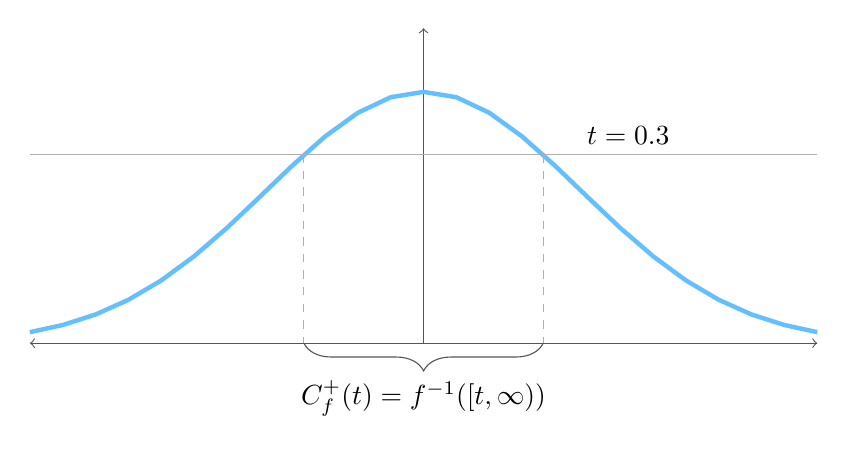
\begin{tikzpicture}[xscale=2,yscale=8]
  % Axes
  \draw[d4black, <->] (-2.5,0) -- (0,0) -- (0,0.5);
  \draw[d4black, ->]  (0,0) -- (2.5,0);
  % Normal PDF
  \draw[d4blue, ultra thick, domain=-2.5:2.5] plot (\x, {(1/sqrt(2*pi))*exp(-pow(\x,2)/2)});
  % Convex set
  \node at (1.3,0.33) {$t=0.3$};
  \draw[d4gray, -]  (-2.5,0.3) -- (2.5,0.3);
  \draw[d4gray, dashed, -]  (-0.76,0.3) -- (-0.76,0);
  \draw[d4gray, dashed, -]  (0.76,0.3) -- (0.76,0);
  \draw[d4black, decorate, decoration={brace, amplitude=10pt, mirror}] (-0.76,0) -- (0.76,0) %
    node[black,midway,yshift=-20pt] {$C_f^+(t) = f^{-1}([t,\infty))$};
\end{tikzpicture}
\end{figure}
\end{ex}

Next, we define the relationship between convex or concave functions and
continuity. In fact, the concepts are deeply related. As the next
theorem will state, convex or concave functions are continuous on the
interior of the domain. This can be seen intuitively enough by looking
at a picture of a convex function with a discontinuity on the domain's
interior.
\begin{figure}[htpb!]
\centering
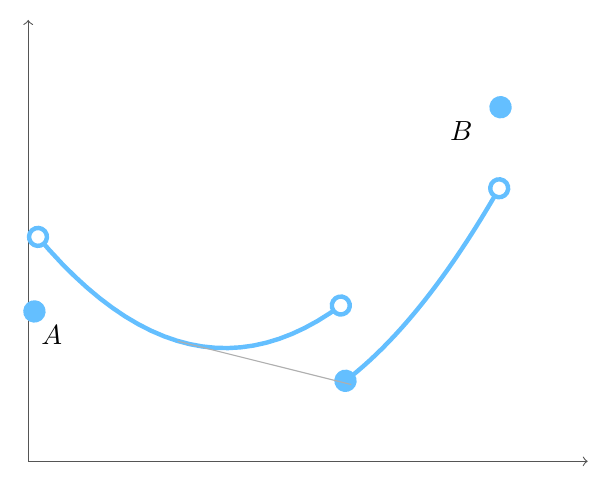
\begin{tikzpicture}[xscale=2, shorten >= -3pt, shorten <= -3pt]
  % Axes
  \draw[d4black, <->] (0,5.5) -- (0,0) -- (3.5,0);

  \draw[d4blue, ultra thick, domain=0.05:0.051, -*] plot (\x, {pow(\x,2)-2.5*\x+2});
  \draw[d4blue, ultra thick, domain=0.05:2, o-o] plot (\x, {pow(\x,2)-2.5*\x+3});
  \draw[d4blue, ultra thick, domain=2:3, *-o] plot (\x, {pow(\x,2)-2.5*\x+2});
  \draw[d4blue, ultra thick, domain=2.99:3, *-] plot (\x, {pow(\x,2)-2.5*\x+3});

  \draw[d4gray, -]  (1,1.5) -- (2,1);

  \node at (0.15,1.60) {$A$};
  \node at (2.75,4.2) {$B$};
\end{tikzpicture}
\end{figure}

As you can see in the figure, around where you have the discontinuity,
you can draw a straight line that lies entirely below the function (in
gray), violating the convexity of the function. Moreover, you can also
see that discontinuities at the \emph{edge} of the domain in the
``appropriate'' direction (like at $B$ rather than $A$) can avoid this
problem. We now make this more explicit in a theorem.

\begin{thm}{\emph{(Convexity/Concavity and Continuity)}}
Given a function $f:C\rightarrow\R$ on convex domain $C$, the function
$f$ is continuous for all $x \in \mathring{C}$, the interior of the
domain.
\end{thm}

\begin{cor}
Given a function $f:C\rightarrow\R$ on convex domain $C$, if $C$ is
open, then $f$ is continuous.
\end{cor}

\subsection{Convexity and Quadratic Forms}

\begin{prop}
Given symmetric matrix $A\in\Rnn$, and quadratic form
$f:\Rn\rightarrow\R$,
\begin{enumerate}
  \item $A$ positive semidefinite $\Rightarrow$ $f$ convex.
  \item $A$ negative semidefinite $\Rightarrow$ $f$ concave.
\end{enumerate}
If you change ``semidefinite'' to ``definite'' in the statements above,
the functions become \emph{strictly} convex or concave.
\end{prop}
\begin{proof}
Suppose that symmetric matrix $A$ is positive semidefinite. By
Theorem~\ref{thm:symmetric-diag}, we can do an eigendecomposition of
matrix $A$ as follows
\begin{align*}
  A = V^T D V = \left(\sqrt{D}V\right)^T \left(\sqrt{D} V\right)
\end{align*}
where $V$ is a matrix of orthogonal eigenvectors and $D$ is a diagonal
matrix of eigenvalues. The matrix $\sqrt{D}$ is simply a real matrix
(because positive semidefinite, see
Theorem~\ref{thm:possemidef-eigenval}) with the roots of the
eigenvalues of $A$ on the diagonal.

We an redefine the function as
\begin{align*}
  f(x) &= (x-b)^T A (x-b) \\
  &= (x-b)^T \left(\sqrt{D}V\right)^T \left(\sqrt{D} V\right)(x-b) \\
  \Rightarrow\quad
  f(x)
  &= \left[N_2\left( \sqrt{D} V(x-b) \right)\right]^2
  := g(N_2(Ax+b'))
\end{align*}
where $N_2$ is the usual Euclidean norm, $g(x)=x^2$, $A=\sqrt{D}V$, and
$b'=-\sqrt{D}Vb$.

Now as a norm, $N_2$ is a convex function. By
Proposition~\ref{prop:coordinvariance}, changing the coordinates
coordinates from $N_2(x)$ to $N_2(Ax+b')$ will still result in a convex
function. Lastly, by Theorem~(TK), taking $g(N_2(Ax+b'))$ for increasing
and convex $g$ will also result in a convex function. So all told, $f$
is convex.
\end{proof}


\subsection{Convexity and Differentiability}

\begin{thm}{\emph{(First Order Condition for Convexity)}}
\label{thm:diffconvex}
Given $f:C\rightarrow \R$ differentiable over its entire open and convex
domain $C\subseteq\Rn$, it follows that the function $f$ is convex if
and only if
\begin{align*}
  f(y) \geq f(x) + [\nabla f(x)]^T (y-x)
  \qquad\forall x,y\in\Rn
\end{align*}
\end{thm}
\begin{proof}
($\Rightarrow$, $n=1$) We want to show that $f$ convex implies that
\begin{align*}
  f(y) \geq f(x) + f'(x)(y-x)
\end{align*}
Since $f$ is convex, for any $\lambda\in(0,1)$ and $x,y\in C$, we have
\begin{align*}
  f(\lambda y + (1-\lambda)x)
  &\leq
  \lambda f(y) + (1-\lambda)f(x) \\
  %\Leftrightarrow \quad
  %f(x + \lambda (y -x))
  %&\leq
  %\lambda f(y) + (1-\lambda)f(x)\\
  \text{Rearranging} \Rightarrow \quad
  f(x + \lambda (y -x))
  - f(x)
  &\leq
  \lambda \left[f(y) - f(x) \right]
\end{align*}
Now divide that last line through by $\lambda(y-x)$ to make this look
more like a derivative, and take the limit as $\lambda\rightarrow 0$:
\begin{align*}
  \lim_{\lambda\rightarrow 0}
  \frac{f(x + \lambda (y -x)) - f(x)}{\lambda(y-x)}
  &\leq
  \frac{f(y) - f(x)}{y-x} \\
  f'(x)
  &\leq
  \frac{f(y) - f(x)}{y-x}\\
  \Leftrightarrow\quad
  f'(x)(y-x) + f(x)
  &\leq
  f(y)
\end{align*}

($\Rightarrow$, $n>1$)
Suppose we have $x,y\in C$. Define the function
\begin{align}
  g(\lambda) = f(\lambda y + (1-\lambda)x)
  \label{eq:gdef}
\end{align}
Then $g(\lambda)$ is a convex function for $\lambda\in [0,1]$.
To see this, you need to dive into some really messy algebra, so
probably don't read this next block of equations.
\begin{align*}
  g(\gamma \lambda_1 + (1-\gamma) \lambda_2)
  &=
  f\big(\; \big[\gamma \lambda_1 + (1-\gamma) \lambda_2\big] \; y
  + \big\{1 - [\gamma \lambda_1 + (1-\gamma) \lambda_2]\big\} x
  \;\big)\\
  \text{Rearranging} \qquad
  &=
  f\big(\;
  \gamma \big[\lambda_1 y - \lambda_1 x\big] \;
  +(1-\gamma)\big[ \lambda_2 y -\lambda_2 x \big]
  +  x
  \;\big)\\
  &=
  f\big(\;
  \gamma \big[\lambda_1 y - \lambda_1 x\big] \;
  +(1-\gamma)\big[ \lambda_2 y -\lambda_2 x \big]
  +  \gamma x + (1-\gamma) x
  \;\big)\\
  &=
  f\big(\;
  \gamma \big[\lambda_1 y + (1- \lambda_1 )x\big] \;
  +(1-\gamma)\big[ \lambda_2 y + (1-\lambda_2) x \big]
  \;\big)\\
  \text{By convexity of $f$}\qquad
  &\leq
  \gamma f(\lambda_1 y + (1- \lambda_1 )x)
  +(1-\gamma)f(\lambda_2 y + (1-\lambda_2) x)
  \\
  \text{By definition of $g$}\qquad
  &\leq
  \gamma g(\lambda_1)
  +(1-\gamma)g(\lambda_2)
\end{align*}
So $g$ is convex.

Now since $g$ is convex, it is the case that
\begin{align}
  g(\lambda_2) - g(\lambda_1)
  \geq g'(\lambda_1)(\lambda_2-\lambda_1)
  \label{ineq:glambda}
\end{align}
To compute $g'(\lambda)$, take $v=\lambda y + (1-\lambda) x$ and apply
the chain rule:
\begin{align}
  g(\lambda) &= f(v)\notag\\
  \Rightarrow\quad
  g'(\lambda)
  &= \sumin f_i(v) \frac{dv_i}{d\lambda}\notag \\
  &= \sumin f_i(\lambda y + (1-\lambda)x) \cdot (y_i-x_i) \notag\\
  \Leftrightarrow \quad
  g'(\lambda)
  &= [\nabla f(\lambda y + (1-\lambda)x)]^T\cdot (y-x)
  \label{eq:gprimelambda}
\end{align}
Okay, so we know how to compute $g'(\lambda)$.

But how do we turn all of this information into a statement about $f$?
Well, notice that Equation~\ref{eq:gdef} relates $g$ to $f$, and in such
a way that we have $g(1)=f(y)$ and $g(0)=f(x)$. So let's take
$\lambda_1=0$ and $\lambda_2=1$, plug into Inequality~\ref{ineq:glambda}
and see what we get:
\begin{align*}
  g(1) - g(0)
  &\geq g'(0)(1-0) \\
  \text{By Equation~\ref{eq:gdef}}\qquad
  f(y)-f(x)
  &\geq g'(0) \\
  \text{By Equation~\ref{eq:gprimelambda}}\qquad
  f(y)-f(x)
  &\geq [\nabla f(x)]^T (y-x) \\
\end{align*}

($\Leftarrow$)
\end{proof}

\begin{thm}{(Second Order Condition for Convexity)}
Given twice-differentiable $f:C\rightarrow\R$ on open and convex domain
$C\rightarrow\R$, we have
\begin{enumerate}
  \item $f$ convex $\iff$ $H_f(x)$ is positive semidefinite for all
    $x\in S$.
  \item $f$ concave $\iff$ $H_f(x)$ is negative semidefinite for all
    $x\in S$.
\end{enumerate}
where $H_f(x)$ is the Hessian matrix of second-order partial derivatives
at $x$. The functions are \emph{strictly} convex or concave if you
swap ``semidefinite'' for ``definite'' in the conditions above.
\end{thm}

\clearpage
\section{Fixed Points}

\subsection{Operators}

\begin{defn}{(Operator)}
If $X$ is some function space
\begin{align*}
  X = \{f:A\rightarrow B\}
\end{align*}
then an \emph{operator}, denoted $T$, is a function
\begin{align*}
  T:X&\rightarrow X \\
  f&\mapsto Tf
  \qquad \forall f\in X
\end{align*}
It is a ``function of functions'', taking elements $f\in X$ and mapping
them to some other element $Tf\in X$. Though of course $T$ is a
function, the word ``operator'' is used to distinguish $T$ from the
functions it acts on.

To avoid overly cumbersome notation, I follow convention and write $Tf$
rather than $T(f)$ when applying operator $T$ to function $f$.
\end{defn}

\begin{ex}
Here's a simple example of an operator $T:X\rightarrow \R$. It acts on
the space of bounded and integrable functions
\begin{align*}
  X = \{f: A\subseteq \R \rightarrow \R\}
\end{align*}
where $A$ is bounded.
The operator is defined
\begin{align*}
  Tf = \int_A f(x) \; dx
\end{align*}
It takes a function $f$, integrates it, and returns a number.
Therefore, $T$ is an operator.
\end{ex}

\subsection{Contraction Maps}

\begin{defn}{(Contraction Map)}
In metric space $(X,d)$, the function $T: X\rightarrow X$ is a
\emph{contraction map} if and only there exists a $\beta \in (0,1)$ such
that
\begin{align*}
  d(T(x), T(y)) < \beta \; d(x,y)
  \qquad x,y\in X
\end{align*}
$\beta$ is called the \emph{modulus} of $T$.
\end{defn}

\begin{prop}{\emph{(Contraction Maps are Continuous)}}
If $T$ is a contraction map, then $T$ is continuous.
\end{prop}
\begin{proof}
Suppose $\varepsilon>0$ given. Then
\begin{align*}
  d(T(x),T(y)) < \beta \; d(x,y)
\end{align*}
Sub in $\delta$ for $d(x,y)$ and solve for $\delta$
\begin{align*}
  \beta \delta = \varepsilon
  \quad\Rightarrow\quad
  \delta = \frac{\varepsilon}{\beta}
\end{align*}
\end{proof}


\begin{thm}{\emph{(Blackwell's Sufficient Conditions for a Contraction)}}
Suppose that we have some operator
$T:\mathscr{B}(X,\R)\rightarrow\mathscr{B}(X,\R)$ on the space of
bounded functions under the sup norm $d_\infty$.
Suppose that $T$ satisfies
\begin{enumerate}
  \item \emph{Monotonicity}: $f(x) \leq g(x)$ for all $x$
    $\implies$ $T[f(x)] \leq T[g(x)]$.
  \item \emph{Discounting}: $T[f(x)+a] \leq T[f(x)] + \beta a$ for some
    $\beta\in(0,1)$.
\end{enumerate}
Then $T$ is a contraction map of modulus $\beta$.
\end{thm}



\subsection{Contraction Mapping Theorem}

\begin{thm}{\emph{(Banach Fixed Point, Contraction Mapping Theorem)}}
\label{thm:banach}
Suppose that $T:X\rightarrow X$ is a contraction map and $(X,d)$ is a
complete metric space. Then
\begin{enumerate}
  \item $\exists! \; x^*$ such that $T(x^*)=x^*$.\footnote{%
      $\exists!$ means ``there exists a unique''}
  \item For all $x_0 \in X$,
    \begin{align}
      \label{thm:fixed-bound1}
      d(T^n(x_0), x^*) \leq \beta^n d(x_0,x^*)
    \end{align}
    where $T^n$ is the contraction map applied $n$ times.

    So applying the contraction map many, many times to any starting
    point $x_0$ will get you closer and closer to the fixed point at
    each iteration.
\end{enumerate}
\end{thm}

\begin{proof}
First, given $x_0$, construct sequence $\{x_n\}$ by defining the $n$th
term to be
\begin{align}
  \label{contraction-map-seq}
  x_n = T^n(x_0)
\end{align}
Now for the proof. It's long, so we do it in parts
\begin{enumerate}
\item
\emph{Show $\{x_n\}$ Converges}:
Let's first prove that $x_n$ converges to \emph{something}. Since the
space $(X,d)$ is complete, it's enough to show that the sequence is
Cauchy.  And to show that $\{x_n\}$ is Cauchy we want to find a bound of
the form
\begin{align*}
  d(x_n,x_m) < G(\min\{m,n\})
\end{align*}
Without loss of generality, suppose that $m\geq n$, or equivalently
$m=n+p$ for some integer $p\geq 0$. Then we can use the triangle
inequality $p$ times to write
\begin{align}
  d(x_n,x_m) = d(x_n,x_{n+p})
  &\leq d(x_n,x_{n+1}) + d(x_{n+1},x_{n+p}) \notag \\
  &\leq d(x_n,x_{n+1}) + d(x_{n+1},x_{n+2}) + d(x_{n+2},x_{n+p})\notag\\
  &\;\; \vdots\notag\\
  &\leq \sum^{p-1}_{i=0} d(x_{n+i},x_{n+i+1})
  \label{fixedpt-series}
\end{align}
Now let's take a look at each of the constituent terms in the
Series~\ref{fixedpt-series} for $i>0$, using the fact that $T$ is a
contraction map:
\begin{alignat*}{3}
  d(x_{n+1},x_{n+2}) &=
  d(T(x_{n}),T(x_{n+1}))
  &&\leq
  \beta d(x_{n},x_{n+1}) \\
  d(x_{n+2},x_{n+3}) &=
  d(T(x_{n+1}),T(x_{n+2}))
  &&\leq
  \beta d(x_{n+1},x_{n+2}) \\
  \vdots \quad & \quad\qquad \vdots
\end{alignat*}
In general, the inequalities above can be summarized as follows:
\begin{align*}
  d(x_{n+i},x_{n+i+1}) &=
  d(T(x_{n+i-1}),T(x_{n+i}))
  \leq
  \beta d(x_{n+i-1},x_{n+i})
  \qquad i = 1,\ldots,p-1
\end{align*}
By recursive substitution for each $i$, we can even bound each term by a
function of $\beta$ and $d(x_n,x_{n+1})$, the first term in
Series~\ref{fixedpt-series}:
\begin{align*}
  d(x_{n+i},x_{n+i+1})
  &\leq
  \beta^i d(x_{n},x_{n+1})
  \qquad i = 1,\ldots,p-1
\end{align*}
This allows us to rewrite Series~\ref{fixedpt-series} and the inequality
for $d(x_n,x_{n+p})$ as
\begin{align}
  d(x_n,x_{n+p})
  \leq \sum^{p-1}_{i=0} d(x_{n+i},x_{n+i+1})
  &\leq \sum^{p-1}_{i=0} \beta^i d(x_{n},x_{n+1})\notag\\
  &\leq  d(x_{n},x_{n+1})\sum^{\infty}_{i=0} \beta^i\notag \\
  \Rightarrow
  d(x_n,x_{n+p})
  &\leq  d(x_{n},x_{n+1})\times \frac{1}{1-\beta}
  \label{fixedpt-ineq}
\end{align}
Okay, that's pretty good. Let's just bound $d(x_n,x_{n+1})$, again using
recursive substitution
\begin{align*}
  d(x_n,x_{n+1})
  = d(T(x_{n-1}), T(x_n))
  &\leq \beta d(x_{n-1}, x_n)\\
  &\leq \beta \cdot \beta d(x_{n-2}, x_{n-1})\\
  &\;\; \vdots \\
  \Rightarrow\quad
  d(x_n,x_{n+1})
  &\leq \beta^n d(x_{0}, x_1)
\end{align*}
Substituting this back into Inequality~\ref{fixedpt-ineq}, we get
\begin{align*}
  d(x_n,x_{n+1})
  &\leq \frac{\beta^n}{1-\beta} d(x_0,x_1)
\end{align*}
Since we want to bound the LHS of the last inequality by $\varepsilon$,
equate and solve for $N$:
\begin{align*}
  \varepsilon &= \frac{\beta^N}{1-\beta} d(x_0,x_1) \\
  \Rightarrow\quad
  N &=
  \frac{1}{\ln \beta}
  \left[
  \ln(1-\beta)+ \ln \varepsilon - \ln(d(x_0,x_1))
  \right]
\end{align*}
This is the choice of $N$ with $\varepsilon$ given.
Therefore $\{x_n\}$ is Cauchy and, since $X$ is complete, convergent.

\item
\emph{Show $x^*$ Exists}: Call $x$ the limit of $\{x_n\}$, which we just
showed exists. In notation, that means
\begin{align*}
  x = \limn x_n = \limn T(x_{n-1})
\end{align*}
By Theorem~\ref{thm:cts-sequential}, the continuity of $T$ means we can
exchange the limit and the function:
\begin{align*}
  x = \limn T(x_{n-1})
  =
  T\left(\limn x_{n-1}\right)
  =
  T\left(x\right)
\end{align*}
Hence, the limit of the sequence $\{x_n\}$ is the fixed point, i.e.\
$x^*=x = \limn x_n$.

\item
\emph{Show Uniqueness}:
Suppose that there were two fixed points $x^*$ and $y^*$. Then
\begin{align*}
  d(x^*, y^*) &= d(T(x^*), T(y^*))
  \quad\text{Since fixed points} \\
  \Rightarrow\quad
  d(x^*, y^*) &\leq \beta d(x^*, y^*)
  \; \quad
  \qquad\text{Since $d(T(x^*), T(y^*)) \leq \beta d(x^*, y^*)$}
\end{align*}
But since $\beta\in (0,1)$, this is impossible unless $d(x^*,y^*)=0$.

\item
\emph{Bound $d(T^n(x_0),x^*)$}:
Similar to what we did above
\begin{align*}
  d(x_n, x^*) = d(T(x_{n-1},T(x^*))
  &\leq \beta d(x_{n-1},x^*)\\
  & \;\; \vdots\\
  &\leq \beta^n d(x_0,x^*)
\end{align*}
\end{enumerate}
\end{proof}

The last theorem is a very useful bit of theory, but we can do a bit
better than the bound given by Inequality~\ref{thm:fixed-bound1}.
Specifically, to be able to tell how far $T^n(x_0)$ is from the fixed
point $x^*$, Theorem~\ref{thm:banach} requires that we know
$d(x_0,x^*)$. Well, a lot of times we don't know. And a lot of times,
we use the contraction mapping theorem to motivate forming a sequence
$T^n(x_0)$ that converges to some fixed point we don't know.
So can we bound $d(T^n(x_0),x^*)$ with stuff we do know?

In fact, we can bound $d(T^n(x_0), x^*)$ by a function of $d(T^n(x_0),
T^{n+1}(x_0))$ instead, which is the change in the sequence
$\{T^n(x_0)\}$. In practical terms, that means ``Keep iterating on the
sequence $\{T^n(x_0)\}$, and if you see that the change in the sequence
from element to element is pretty small, you can be confident that
you're close to the fixed point.'' You don't have to know what the fixed
point is. You just need to compute $T^{n+1}(x_0) - T^n(x_0)$, which is
always feasible, in general. This is the next result.
\begin{cor}
Consider contraction map $T:X\rightarrow X$ with modulus $\beta$ in
complete metric space $(X,d)$. Given any starting point $x_0\in X$,
\begin{align*}
  d(T^n(x_0), x^*)
  \leq \frac{d(T^n(x_0),T^{n+1}(x_0))}{1-\beta}
\end{align*}
\end{cor}
\begin{proof}
Again, form the sequence $\{x_n\}$ as we did above in
(\ref{contraction-map-seq}).
\begin{align*}
  x_n = T^n(x_0)
\end{align*}
The goal is to bound the distance between $T^n(x_0)$ and $x^*$ using
only information about the change
\begin{align*}
  d(T^n(x_0), x^*)
  &\leq
  G\left(\;d(T^n(x_0), T^{n+1}(x_0))\;\right)\\
  \Leftrightarrow\qquad
  d(x_n, x^*)
  &\leq
  G\left(\;d(x_n, x_{n+1})\;\right)
\end{align*}
Using the triangle inequality, the fact that $T$ is a contraction map,
and the fact that $x^*$ is a fixed point,
\begin{align*}
  d(x_n, x^*)
  &\leq d(x_n,x_{n+1}) + d(x_{n+1},x^*) \\
  &\leq d(x_n,x_{n+1}) + d(T(x_n),T(x^*)) \\
  &\leq d(x_n,x_{n+1}) + \beta d(x_n,x^*) \\
  \Rightarrow\quad
  d(x_n, x^*)
  &\leq \frac{d(x_n,x_{n+1})}{1-\beta}
\end{align*}
Since $d(x_n,x^*)=d(T^n(x_0),x^*)$, we have the desired result.
\end{proof}

\begin{defn}{($T$-Invariant Sets)}
Given an operator/function $T:X\rightarrow X$ and some set $C\subseteq
X$, we say that the set $C$ is \emph{$T$-invariant} if
\begin{align*}
  T(C)\subseteq C
\end{align*}
\end{defn}

\begin{prop}
Suppose that $T: X\rightarrow X$ is a contraction map for complete space
$X$. Let $x^*$ denote the unique fixed point. Then
\begin{enumerate}
  \item If $C\subseteq X$ is a closed, nonempty, $T$-invariant set, then
    $x^* \in C$.
  \item If $C' \subseteq C \subseteq X$ where $C$ is closed but $C'$ is
    an arbitrary subset such that $T(C) \subseteq C'$, then $x^* \in
    C'$.
\end{enumerate}
\end{prop}
\begin{proof}
(Part 1) Start with some $x_0\in C$. Since $C$ is $T$-invariant,
$T^n(x_0) \in C$ for all $n$. Moreover, by Theorem~\ref{thm:banach},
the sequence $\{T^n(x_0)\}\subseteq C$ converges to $x^*$. Since $C$ is
closed, the set must contain its limit point by
Proposition~\ref{prop:closed}, hence $x^*\in C$.

(Part 2) Again, the assumptions of this part imply that $C$ is
$T$-invariant since $T(C)\subseteq C' \subseteq C$.  And since $C$ is
closed, $x^*\in C$ by Part 1.

Finally, by assumption $T(x) \in C'$ for all $x \in C$, and we just said
$x^*\in C$. So $T(x^*)\in C'$ too.
\end{proof}

\subsection{Brouwer's Fixed Point Theorem}

\begin{thm}
Suppose that $T:K\rightarrow K$ is a continuous function and $K\subseteq
\Rn$ is compact and convex.  Then there exists a fixed point
such that $x^*=T(x^*)$.
\end{thm}
\begin{rmk}
There are three key differences from Theorem~\ref{thm:banach}---the
Contraction Mapping or Banach Fixed Point Theorem.
\begin{enumerate}
  \item $T$ need not be a contraction map. It only needs to be a
    continuous function (which is weaker).
  \item We provide no way to construct a sequence that converges to the
    fixed point.
  \item The fixed point need not be unique. The theorem just furnishes
    existence.
\end{enumerate}
\end{rmk}


\clearpage
\section{Optimization in $\Rn$}

\subsection{The Canonical Optimization Problem}

Throughout this section, we will consider optimization problems for
scalar-valued functions on domain $\Rn$. The problems we consider will
be of the form
\begin{alignat}{3}
  \text{Objective Function:} \qquad
    && \max_{x\in\mathcal{D}} \; &f_0(x) \label{prob:max}\\
  \text{Inequality Constraints:} \qquad
    && \text{s.t.} \; &f_i(x) \geq 0 \qquad i = 1,\ldots, m\notag \\
  \text{Equality Constraints:} \qquad
    && &g_i(x) = 0 \qquad i = 1,\ldots,k\notag
\end{alignat}
where the domain of the problem $\mathcal{D}$ is defined as the
intersection of the domains of all constituent functions
\begin{align*}
  \mathcal{D} = \dom(f_0)
  \cap \left( \bigcap^m_{i=1} \dom(f_i)\right)
  \cap \left( \bigcap^k_{i=1} \dom(g_i)\right)
\end{align*}
where $\dom(f)$ refers to the domain of function $f$. Generally, I will
assume that the domains of $f_0$, $f_i$, and $g_i$ are open for all $i$,
which implies that $\mathcal{D}$---a finite intersection of open
sets---is open as well.

\paragraph{Terminology and Notation}
\begin{enumerate}
  \item \emph{Feasible Point}, $x\in\mathscr{F}_p$: Any point
    $x\in\mathcal{D}$ satisfying all of the inequality and equality
    constraints.
  \item \emph{Feasible Set}, $\mathscr{F}_p$: The set of all feasible
    points.
  \item \emph{Optimal Value}, $p^*$: The maximal value of the problem,
    over the feasible set $\max_{x\in \mathscr{F}_p} f_0(x)$.
  \item \emph{Optimal Point}, $x^*$: Any feasible point
    $x^*\in\mathscr{F}_p$ such that $f_0(x^*)=p^*$.
\end{enumerate}
I will collectively refer to this entire problem as either
Problem~\ref{prob:max}, the ``Canonical Optimization Problem'', or the
``Primal Problem'' (in contrast to the ``Dual Problem'' which will be
introduced later). Solving Problem~\ref{prob:max} will be the goal of
this entire section. I will proceed by starting with some general
results about extrema, which correspond to solving
Problem~\ref{prob:max} without any constraints---simple unconstrained
optimization over a function's entire domain, given particular
assumptions about $f$. I will then introduce the notion of the ``Dual
Problem'', which simply turns Problem~\ref{prob:max} into a different
(often simpler and equivalent) optimization problem. I will then offer
some intuition, examples, and applications under equality and inequality
constraints.

But it's important to note that I am currently assuming nothing about
the underlying functions that define the problem---not continuity,
differentiability, concavity, convexity, etc. Of course, these
assumptions will factor in later, since we often use continuity to
ensure existence of a maximum or concavity/convexity to ensure
uniqueness. \emph{However}, we will also derive many useful results
where we impose no assumptions on the problem. So any assumptions will
generally be made very explicit, and I will present throughout this
section a mix assumption-free and assumption-heavy results.

\subsection{Concave Programming Problem}

In this section, I introduce a special case of Problem~\ref{prob:max}
that is particularly well behaved. Specifically, the problem is as
before with additional assumptions on the constraints:
\begin{alignat}{3}
  \text{Concave Objective Function:} \qquad
    && \max_{x\in\mathcal{D}} \; &f_0(x) \label{prob:maxconcave}\\
  \text{Concave Inequality Constraints:} \qquad
    && \text{s.t.} \; &f_i(x) \geq 0 \qquad i = 1,\ldots, m\notag \\
  \text{Affine Equality Constraints:} \qquad
    && &a_i^T x = b_i \qquad i = 1,\ldots,k\notag
\end{alignat}
I will collectively refer to this as Problem~\ref{prob:maxconcave}, or
the ``Concave Programming Problem.''

\subsection{Extrema: Definitions and Facts}
\label{sec:extrema}

In this section, I cover some basic results about extrema of functions.
Note that I do not necessarily assume functions are differentiable.
Unless differentiability is explicitly stated, a result holds generally.

\begin{defn}{(Local Maximum)}
For function $f:S\subseteq\Rn\rightarrow \R$, we say that $\bar{x} \in
S$ is a \emph{local maximum} if there exists an $\varepsilon>0$ such
that
\begin{align*}
  f(\bar{x})\geq f(y)
  \qquad \forall y \in B_\varepsilon(x) \cap S
\end{align*}
\end{defn}

\begin{prop}{\emph{(Derivatives at Extrema)}}
Given function $f:S\subseteq \Rn\rightarrow \R$ on open set $S$, suppose
that $\bar{x}$ is a local max of $f$ and that the partial derivative
$f_i(\bar{x})$ exists.  Then $f_{i}(\bar{x})=0$.
\end{prop}

\begin{note}
First, the converse does not hold. Saddle points have $f_i(x)=0$ for all
partial derivatives, but they are not extrema. In other words, the
condition $f_i(\bar{x})=0$ is necessary but not sufficient for $\bar{x}$
to be a local maximum. Only if we impose regularity conditions on the
function will this be sufficient.

Second, I'm not saying that the partial derivative \emph{will} exist or
that the function is differentiable. I'm saying that \emph{if it is
differentiable} or \emph{if the partial does exist}, then it must equal
zero.
The next definition concerns itself with functions that are, in
fact, differentiable everywhere in the domain.
\end{note}

\begin{defn}{(Critical Point)}
Suppose that $f:S\rightarrow\R$ is a differentiable function on open set
$S\in\Rn$. The point $x^*\in\Rn$ is called a \emph{critical
point} of $f$ if
\begin{align*}
  \nabla f(x^*) = 0
  \quad\text{or equivalently}\quad
  f_i(x^*)=0
  \quad\forall i=1,\ldots,n
\end{align*}
Take note, critical points as defined above are a concept dependent upon
differentiability.
\end{defn}

\subsection{Extrema and Concave Functions}
\label{sec:extrema-concave}

\begin{prop}{\emph{(Extrema of Differentiable Concave Functions)}}
Suppose that $f:C\rightarrow\R$ is a differentiable and concave function
on convex and open domain $C\subseteq\Rn$. Then if $x^*$ is a critical
point of $f$ (i.e.\ $\nabla f(x^*)=0$), we have
\begin{align*}
  x^* \in \arg\max_{x\in C} f(x)
\end{align*}
For $f$ \emph{strictly} concave, $x^*$ is is a \emph{unique} global max.
\end{prop}
\begin{proof}
By Theorem~\ref{thm:diffconvex} (but flipped since $f$ is now concave),
we know that
\begin{align*}
  f(y) \leq f(x) + [\nabla f(x)]^T (y-x)
  \qquad \forall x,y\in C
\end{align*}
Since $x^*$ is a critical point, $\nabla f(x^*)=0$. Now use that as $x$
in the inequality above to get, for all $y\in C$,
\begin{align*}
  f(y) &\leq f(x^*) + [\nabla f(x^*)]^T (y-x^*)
  = f(x^*) + 0\\
  \Rightarrow\; \forall y\in C\qquad
  f(y) &\leq f(x^*)
\end{align*}
Hence $x^*$ is a maximum.
\end{proof}

\begin{prop}{\emph{(Extrema of Arbitrary Concave Functions)}}
Suppose that we have a concave function $f:C\rightarrow \R$ defined on
convex domain $C$. Define $X^*\subseteq C$ as the set of ``maximizing
points'' in $C$.
\begin{align*}
  X^* = \arg\max_{x\in C} f(x)
  = \{ x \in C \; | \; f(y) \leq f(x) \quad \forall y \in C\}
\end{align*}
Then
\begin{enumerate}
  \item $X^*$ is a convex set.
  \item $f$ strictly concave and $X^*\neq \emptyset$ implies that $X^*$
    consists of a single point, a \emph{unique} maximizer.
\end{enumerate}
\end{prop}
\begin{proof}
%($X^*$ Convex) Suppose $X^*=\emptyset$. The empty set is convex so done.
%Now suppose that $X^*$ is nonempty. Choose any $x,y\in X^*$.  It must be
%the case that $f(x) = f(y)$, otherwise the smaller of the two would not
%be a maximizer of the function and, therefore, not in $X^*$. So define
%$f^* = f(x) = f(y)$.

%Now to draw a contradiction, suppose that $X^*$ is not convex. That
%means there exists a $\lambda$ such that
%\begin{align*}
  %z_\lambda = \lambda x + (1-\lambda)y \not\in X^*
%\end{align*}
%Since $z_\lambda \not\in X^*$, it is not a maximizer. Therefore
%\begin{align*}
  %f(z_\lambda) &< f^* = \lambda f^* + (1-\lambda)f^* \\
  %\Rightarrow\quad
  %f(\lambda x + (1-\lambda)y) &< \lambda f(y) + (1-\lambda)f(y) \\
%\end{align*}
%But that's a contradiction since we assumed $f$ is concave.

(Part 1, $X^*$ Convex) Suppose $X^*=\emptyset$. The empty set is convex
so done.  Now suppose that $X^*$ is nonempty. Choose any $x,y\in X^*$.
It must be the case that $f(x) = f(y)$, otherwise the smaller of the two
would not be a maximizer of the function and, therefore, not in $X^*$.
So define $f^* = f(x) = f(y)$.  Then $X^* = C^+_f(f^*)$, which is a
convex set whenever $f$ is concave by
Proposition~\ref{prop:convexfcnset}.

(Part 2, Uniqueness for Strictly Concave $f$)
Suppose $X^*$ consists of more than one distinct point. Then take any
two $x,y\in X^*$. As before $f(x)=f(y)=f^*$ for some $f^*$, othwerise
the smaller of the two would not be a maximizer.

Now take any $\lambda\in(0,1)$ and construct
\begin{align*}
  z_\lambda = \lambda x + (1-\lambda)y
\end{align*}
Since $X^*$ is convex by the first part of the proof, $z_\lambda\in
X^*$. Moreover, since $f$ is strictly concave, by the definition of
strict concavity,
\begin{align*}
  f(\lambda x + (1-\lambda) y)
  &>
  \lambda f(x) + (1-\lambda) f(y) \\
  \Leftrightarrow \quad
  f(z_\lambda) &> \lambda f^* + (1-\lambda) f^* = f^* \\
  \Rightarrow\quad
  f(z_\lambda) &> f^*
\end{align*}
In summary, $z_\lambda \in X^*$ and it's bigger than both $x$ and $y$.
That contradicts our definitions of $X^*$ and $f^*$.
\end{proof}

\subsection{The Lagrangian and the Lagrange Dual Function}

\begin{defn}{(Lagrangian)}
Given Problem~\ref{prob:max}, define the \emph{Lagrangian}
\begin{align*}
    \sL(x,\lambda,\mu)
    := f_0(x)
    + \sum^m_{i=1} \lambda_i f_i(x)
    + \sum^k_{i=1} \mu_i g_i(x)
\end{align*}

where vectors $\lambda$ and $\mu$ are called the \emph{Lagrange
multipliers}. Overall, $\sL$ is a function of $n+m+k$ variables since
$x\in\Rn$, $\lambda\in\mathbb{R}^m$, and $\mu\in\mathbb{R}^k$
\end{defn}

As explained in Boyd,\footnote{This is reproduced essentially verbatim
because I liked their explanation so much. Go read their book for an
even better and more detailed explanation}.  we can interpret the
Lagrangian as a linear approximation of Problem~\ref{prob:max}.
Specifically, we want to maximize $f_0$ subject to the constraints.
Well, if we introduce functions that impose an infinite penalty to
violating the constraints, we can write the maximization problem in one
line:
\begin{align}
  \label{prob:linapprox}
  \max_{x\in\mathcal{D}} \;
  f_0(x) + \sum^m_{i=1} I_+(f_i(x))
  + \sum^k_{i=1} I_0(g_i(x))
\end{align}
where
\begin{align*}
  I_+(y) =
  \begin{cases}
    -\infty & y < 0 \\
    0 & y \geq 0
  \end{cases}
  \qquad
  I_0(y) =
  \begin{cases}
    -\infty & y \neq 0 \\
    0 & y = 0
  \end{cases}
\end{align*}
So if you violate the constraints, you get an infinite penalty.  In
trying to maximize objection function of Problem~\ref{prob:linapprox},
we see that the optimization will result in an $x\in\mathcal{D}$ that
avoids the infinite penalties, and so satisfies the constraints.

The Lagrangian is quite similar to the objective function in
Problem~\ref{prob:linapprox}. But instead of using an infinite penalty,
it introduces a \emph{linear} penalty for some vectors $\lambda$ and
$\mu$.

\begin{defn}{(Lagrange Dual Function)}
Given canonical Problem~\ref{prob:max} and corresponding Lagrangian
$\sL(x,\lambda,\mu)$, define the \emph{Lagrange dual function}, or
simply the \emph{dual}, as
\begin{align*}
  g(\lambda,\mu) = \sup_{x\in\mathcal{D}} \; \sL(x,\lambda,\mu)
  = \sup_{x\in\mathcal{D}}
    \left\{ f_0(x)
    + \sum^m_{i=1} \lambda_i f_i(x)
    + \sum^k_{i=1} \mu_i g_i(x)
    \right\}
\end{align*}
If the sup does not exist, simply define $g(\lambda,\mu)=+\infty$.
Here, $\lambda$ and $\mu$ are parameters.
\end{defn}

The Lagrange dual function is hugely important because it is
well-behaved and extrema of the dual provide a lot of information about
the problem we really want to solve, Problem~\ref{prob:max}.  First,
while we generally have no guarantees \emph{a priori} about the shape of
the objective function or the Lagrangian (unless we impose restrictive
assumptions on $f_0$, $f_i$, and $g_i$), we will see that the Lagrange
dual function is \emph{always} convex. So we can find extrema of the
dual by applying many of the nice results that we saw in
Section~\ref{sec:extrema-concave} for extrema of convex and concave
functions without assuming anything. Second, we can use the dual to
bound from above the optimal vlaue $p^*$ of Problem~\ref{prob:max}.
Now let's turn all of these wildly ludicrous and unbelievable claims
into formal statements.

\begin{thm}{\emph{(Dual as Bound)}}
\label{thm:dual-bound}
For any point $x\in\mathscr{F}_p$ in the feasible set of
Problem~\ref{prob:max} and $\lambda\geq 0$, we have
\begin{align}
  f_0(x) \leq g(\lambda,\mu)
  \label{ineq:dual-bound-f}
\end{align}
Moreover, given optimal value $p^*$,
\begin{align}
  p^* \leq g(\lambda,\mu)
  \label{ineq:dual-bound-p}
\end{align}
So even if we don't know the max $p^*$, we can bound it.
\end{thm}

\begin{proof}
Take feasible point $x\in \mathscr{F}_p$. By the definition of
feasibility it satisfies the constraints. So first,
\begin{align*}
  g_i(x)=0 \; \forall i
  \implies
  \sum_{i=1}^k g_i(x) = 0
\end{align*}
Next, since $\lambda\geq 0$,
\begin{align*}
  f_i(x) \geq 0 \; \forall i
  \implies
  \sum_{i=1}^m f_i(x) \geq 0
\end{align*}
So in adding these two things to $f_0(x)$, we can only increase the
value of the sum:
\begin{align*}
  f_0(x) \leq f_0(x)
  + \underbrace{\sum_{i=1}^m f_i(x)}_{\geq 0}
  + \underbrace{\sum_{i=1}^k g_i(x)}_{=0}
\end{align*}
Finally, take the sup of the object on the righthand side of the
inequality---which can only increase the value---and you end up with
$g(\lambda,\mu)$, proving Inequality~\ref{ineq:dual-bound-f}. Taking the
sup over $f_0(x)$ on the lefthand side too gives $p^*$, proving
Inequality~\ref{ineq:dual-bound-p}.
\end{proof}

\begin{thm}{\emph{(Dual Convex)}}
\label{thm:dual-convex}
Given Canonical Optimization Problem~\ref{prob:max}, the Lagrange dual
function $g(\lambda,\mu)$ is \emph{convex}, even without any assumtions
on functions $f_0$, $f_i$, or $g_i$.
\end{thm}
\begin{proof}
Given $x\in\mathcal{D}$, define
\begin{align*}
  \varphi_x(\lambda,\mu) = f_0(x)
    + \sum^m_{i=1} \lambda_i f_i(x)
    + \sum^k_{i=1} \mu_i g_i(x)
\end{align*}
This function is an affine function of $\lambda$ and $\mu$. Therefore,
it is both concave and convex. So we are correct in saying that
$\{\varphi_x\}_{x\in\mathcal{D}}$ is a family of concave functions, so
\begin{align*}
  g(\lambda,\mu) = \sup_{x\in\mathcal{D}} \varphi_x(\lambda,\mu)
\end{align*}
will be convex by Proposition~\ref{prop:supconvex} since
$g(\lambda,\mu)$ is the the supremum of a family of convex functions.

\end{proof}

\subsection{The Dual Problem to the Canonical Optimization Problem}

Suppose you have Canonical Optimization Problem~\ref{prob:max}. If that
is the \emph{primal} problem, you can always write down and solve the
\emph{dual} problem which, not surprisingly, involves working with the
Lagrange dual function for the problem. Often, this is much easier to
solve, so I now lay out that problem explicitly, just like
Problem~\ref{prob:max}.

Given Canonical optimization Problem~\ref{prob:max} and corresponding
dual function $g(\lambda,\mu)$, define the \emph{Dual Problem}
\begin{align}
  \label{prob:dual}
  \min_{\lambda,\mu} \; &g(\lambda,\mu) \\
  \text{s.t.} \; &\lambda \geq 0\notag
\end{align}
where $\lambda\in\R^m$ and $\mu\in\R^k$.
Since $g(\lambda,\mu)$ is convex by Theorem~\ref{thm:dual-convex}, this
is a nice, well-behaved optimization problem to solve.

\paragraph{Terminology and Notation}
\begin{enumerate}
  \item \emph{Dual Feasible}, $(\lambda,\mu)\in\mathscr{F}_d$: Pair
    $(\lambda,\mu)$ is ``dual feasible'' if $\lambda\geq 0$.
  \item \emph{Dual Value}, $d^*$: The optimum of
    Problem~\ref{prob:dual}, $d^* = \min_{(\lambda,\mu)\in\mathscr{F}_d}
    g(\lambda,\mu)$
  \item \emph{Weak Duality}, $p^*\leq d^*$: This follows immediately
    from Theorem~\ref{thm:dual-bound}, where $p^*$ is the optimal point
    of primal Problem~\ref{prob:max}.
  \item \emph{Strong Duality}, $p^*=d^*$: This does not hold in general,
    but we care about precisely those cases where it does because of the
    next theorem.
  \item \emph{Duality Gap}, $p^*-d^*$: Positive number corresponding to
    difference of primal and dual optimal values. No duality gap if and
    only if strong duality.
\end{enumerate}

\begin{thm}{\emph{(Bounding Suboptimality)}}
Given Canonical Problem~\ref{prob:max}, corresponding Lagrange dual
function $g(\lambda,\mu)$, the primal and dual optimal values $p^*,
d^*$, and any primal and dual feasible triplet $(x,\lambda,\mu)$ with
$x\in\mathscr{F}_p$ and $(\lambda,\mu)\in\mathscr{F}_d$, we can bound
suboptimality as follows
\begin{align*}
  0 \leq \underbrace{p^* - f_0(x)}_{\text{Suboptimality}}
  \leq d^* - f_0(x)
  \leq g(\lambda,\mu) - f_0(x)
\end{align*}
Hence $p^*\in [f_0(x), d^*]$, and $d^*\in[f_0(x),g(\lambda,\mu)]$.
\end{thm}
\begin{rmk}
This theorem is incredible! Without knowing $p^*$---the optimal value of
the primal problem that you really want to find---you can bound how far
away you are. For any (repeat: \emph{any}) problem in Canonical
Representation~\ref{prob:max} (with zero assumptions), if I know the
dual $g(\lambda,\mu)$ and the objective function $f_0(x)$, I can tell
how far away $f_0(x)$ is from the optimal value $p^*$ that I am trying
to find. And in general, we \emph{always} know $g(\lambda,\mu)$ and
$f_0(x)$. Moreover, we can establish the tightest bound by solving the
convex Dual Problem~\ref{prob:dual} for $d^*$.

Moreover, this provides a nice stopping-criterion when solving
Problem~\ref{prob:max} with a computer. Specifically, if we want to find
an $x^*$ such that $f_0(x^*)$ is
no more than $\varepsilon$ units away from  optimum $p^*$, try different
values of $x$ (hopefully in some algorithmic, intelligent, sequential
way). At each step, compute $f_0(x)$ and $d^*$ (or $g(\lambda,\mu)$) at
each iteration, check the bound $p^*-f_0(x)$, and stop if this is
guaranteed to be less than $\varepsilon$.
\end{rmk}

\begin{defn}{(Slater's Condition)}
Given Canonical Problem~\ref{prob:max}, we say that the problem
satisfies \emph{Slater's condition} if there exists at least one
$\hat{x}\in\mathscr{F}_p$ such that
\begin{align*}
  f_i(\hat{x})>0
  \quad \forall i=1,\ldots,m
\end{align*}
In words, there exists at least one point interior to the feasible set
of the problem (i.e.\ not on the boundary for any inequality
constraint).
\end{defn}

\begin{thm}{\emph{(Slater's Theorem)}}
If you have Concave Programming Problem~\ref{prob:maxconcave} and it
satisfies Slater's Condition, then you have strong duality, i.e.\
$p^*=d^*$.

In words, the existence of at least one point interior to the primal
feasible set (not on the boundary for any primal constraint) guarantees
strong duality.
\end{thm}

\subsection{KKT Conditions}

Suppose that you have a point $x^*$ in the domain of
Problem~\ref{prob:max}.  How can you easily check if it is optimal, or
rule it out as suboptimal? In other words, what are some necessary or
sufficient conditions that $x^*$ must satisfy if it really is an
optimum?  In some cases, the answer is the Karush-Kuhn-Tucker (KKT)
Conditions.

The KKT conditions are a set of sometimes-necessary, sometimes-sufficent
conditions that are useful for characterizing solutions to nonlinear
optimization problems in the form of Problem~\ref{prob:max}. When
exactly they are necessary and when exactly they are sufficient is
complicated, so special care will be taken to note this explicitly.
But first, we state the KKT conditions (along with some intuition),
before deriving them explicitly.

%, but there are also certain ``Constraint Qualifications''
%(CQ) or regularity conditions that the point must meet for the KKT
%Conditions to be necessary.  More compactly
%\begin{align*}
  %\text{$x^*$ satisfies CQ}
  %\implies
  %\text{KKT conditions necessary for $x^*$ to be an optimum}
%\end{align*}
%``Constraint Qualifications'' (CQ) are restrictions that rule out weird
%irregular cases where $x^*$ is an optimal point at the boundary of the
%constraint set but $x^*$ \emph{does not} satisfy the KKT conditions.
%Again, if CQ are satisfied, then the Karush-Kuhn-Tucker (KKT) Conditions
%are a set of \emph{first order} \emph{necessary} conditions that must
%hold for $x^*$ to be an optimal point of Problem~\ref{prob:max}.

%This suggests a way to test if $x^*$ is an optimal point of
%Problem~\ref{prob:max}. Specifically, $x^*$ is an optimum if either
%\begin{enumerate}
  %\item Point $x^*$ satisfies some constraint qualifications and the
    %consequently necessary KKT conditions.
  %\item Point $x^*$ does not satisfy some constraint qualifications, so
    %$x^*$ could still be an optimum though the KKT conditions might not
    %be satisfied.
%\end{enumerate}
%Therefore, to find optima, examine points where both the KKT conditions
%\emph{hold} and points where CQ fails.

%Note, that I've said nothing about sufficiency. Constraint
%qualifications and the KKT conditions only concern necessary conditions.
%We'll have to say more to guarantee sufficiency (and I will below).

\begin{defn}{(KKT Conditions)}
Given optimal canonical optimization Problem~\ref{prob:max},
$(x^*,\lambda^*,\mu^*)$ satisfies the KKT conditions if all of the
following hold:
\begin{enumerate}
  \item \emph{$x^*$ Stationary point of Lagrangian}:
    \begin{align*}
      0 &= \nabla_x \sL(x^*,\mu^*,\lambda^*)
        = \nabla_x f_0(x^*)
        + \sum^m_{i=1} \lambda_i^* \; \nabla_x f_i(x^*)
        + \sum^k_{i=1} \mu_i^* \; \nabla_xg_i(x^*)
    \end{align*}
  \item \emph{Primal feasibility}, $x^*\in \mathscr{F}_p$: $x^*$ is a
    feasibile point, satisfying all constraints of primal
    Problem~\ref{prob:max}
    \begin{align*}
      x^*\in \mathscr{F}
      \implies
      \begin{cases}
        f_i(x^*)\geq 0 & i = 1,\ldots,m\\
        g_i(x^*)= 0 & i = 1,\ldots,k
      \end{cases}
    \end{align*}

  \item \emph{Dual Feasibility}, $(\lambda^*,\mu^*)\in\mathscr{F}_d$:
    Pair $(\lambda^*,\mu^*)$ is a feasible point, satisfying all
    constraints of Dual Problem~\ref{prob:dual}
    \begin{align*}
      \lambda^*_i \geq 0
      \qquad i=1,\ldots,m
    \end{align*}

  \item \emph{Complementary Slackness}: For inequality constraint $i$,
    either the inequality is binding so $f_i(x^*)=0$, or it's not
    binding and multiplier $\lambda^*_i=0$. That can be encapsulated in
    one line as
    \begin{align}
      \label{kkt:slackness}
      \lambda_i^* f_i(x^*) =0
      \qquad i=1,\ldots,m
    \end{align}
     %Recall the interpretation of the multipliers: $\lambda_i^*$ is how
     %much the objective function would increase if constraint $i$ were
     %relaxed.  Well, if the constraint is non-binding, $f_i(x^*)>0$ and
     %the objective function wouldn't change after relaxing that
     %constraint.  So $\lambda_i^*$ should be zero. And if inequality
     %constraint $i$ binds, then $f_i(x^*)=0$ so $\lambda^*_i$ can be any
     %finite number So Equation~\ref{kkt:slackness} provides a nice
     %one-line encapsulation of these two possibilities.
\end{enumerate}
Now we move on to some theorems and results that tell us about when the
conditions are necessary, sufficient, or both.
\end{defn}

\begin{thm}{\emph{(Primal Solution $+$ Strong Duality $\implies$ Dual
Solution \& KKT Necessary)}}
Suppose that strong duality holds.  If $x^*\in\mathscr{F}_p$ solves
Problem~\ref{prob:max}, then there exist
$(\lambda^*,\mu^*)\in\mathscr{F}_d$ solving the Dual
Problem~\ref{prob:dual} such that $(x^*,\lambda^*,\mu^*)$ satisfy the
KKT conditions.
\end{thm}
\begin{proof}
Since $x^*\in\mathscr{F}_p$ solves the problem, it trivially satisfies
KKT Condition 2, Primal Feasibility.

Next, since $x^*$ solves the primal problem, $f_0(x^*)=p^*$. By strong
duality, $d^*=p^*$ exists so the dual problem has a solution. Since
$d^*$ exists and the dual problem has a solution, we can choose
\begin{align}
  \label{eq:pick-lambda-mu}
  (\lambda^*,\mu^*) \in \mathscr{F}_d
  \quad \text{such that}
  \quad g(\lambda^*,\mu^*) = d^*
\end{align}
Since $(\lambda^*,\mu^*)\in\mathscr{F}_d$, we also know $\lambda^*\geq
0$, satisfying KKT Condition 3, Dual Feasibility.

Next, we can chain together
%since $\lambda^*\geq 0$ and $x^*\in\mathscr{F}_p$ satisifies all
%of the constraints,
\begin{align*}
  \text{Since $x^*$ solves primal} \qquad p^* &= f_0(x^*) \\
  \text{Since $x^*\in\mathscr{F}_p$ and $\lambda^*\geq 0$} \qquad
  &\leq f(x^*) + \sum^m_{i=1} \lambda^* f_i(x^*)
  + \sum^k_{i=1} \mu_i^* g_i(x^*) \\
  \text{By definition of sup} \qquad
  &\leq \sup_{x\in D} f(x) + \sum^m_{i=1} \lambda^* f_i(x)
  + \sum^k_{i=1} \mu_i^* g_i(x) \\
  \text{By definition of $g(\lambda,\mu)$} \qquad
  &= g(\lambda^*,\mu^*) \\
  \text{By Equation~\ref{eq:pick-lambda-mu}'s
    choice of $(\lambda^*,\mu^*)$} \qquad &= d^* \\
  \text{By strong duality}\qquad
  &= p^*\\
  \text{Since $x^*$ solves primal}\qquad
  &= f_0(x^*)
\end{align*}
Buried in that chain is the squeezing
\begin{align*}
  p^*
  &\leq f_0(x^*) + \sum^m_{i=1} \lambda^* f_i(x^*)
  + \sum^k_{i=1} \mu_i^* g_i(x^*)
  \leq p^*
\end{align*}
Since $f(x^*)=p^*$ and the equality constraints are defined to equal
zero for feasible $x^*$ (i.e.\ $\sum^k_{i=1}\mu^*_ig_i(x^*)=0$), it must
also be the case that
\begin{align*}
  \sum^m_{i=1} \lambda^* f_i(x^*)
  =0
\end{align*}
Hence, we satisfy KKT Condition 4, Complementary Slackness.

Lastly, also buried in that chain is
\begin{align}
  f_0(x^*)
  = f_0(x^*) + \sum^m_{i=1} \lambda^* f_i(x^*)
  + \sum^k_{i=1} \mu_i^* g_i(x^*)
  = \sup_{x\in D} f_0(x) + \sum^m_{i=1} \lambda^* f_i(x)
  + \sum^k_{i=1} \mu_i^* g_i(x)
  \label{kkt:criticalproof}
\end{align}
Now think of the guy on the very right as a function of $x$ only, where
$(\lambda^*,\mu^*)$ are fixed---call it
$\sL_{\lambda^*,\mu^*}(x):=\sL(x,\lambda^*,\mu^*)$.
Equation~\ref{kkt:criticalproof} effectively says that
$x^*\in\mathcal{D}$ maximizes $\sL_{\lambda^*,\mu^*}(x)$, so the sup is
really a max. Since the domain $\mathcal{D}$ is an open set and since
the point maximizes the function, it must be the case that
\begin{align*}
  0 &= \nabla_x \sL_{\lambda^*,\mu^*}(x^*)
  =:
  \nabla_x \sL(x^*,\lambda^*,\mu^*)
\end{align*}
And that's precisely KKT Condition 1, implying $x^*$ is a stationary
point of the Lagrangian.

\end{proof}


\subsection{Equality Constraints}

\subsubsection{Single Constraint}
Suppose that for vector $x$ and scalar-valued differentiable functions
$f$ and $g$, we are faced with the problem
\begin{align}
  \max_x &f(x) \label{prob:eqconst}\\
  \text{s.t. } &g(x) = 0 \notag
\end{align}
If this were an \emph{unconstrained} optimization, we'd just find the
point(s) in the domain of $f$ where $f'(x)=0$, i.e.\ where $f$ doesn't
change in a small neighborhood about $x$.
\\
\\
But since this is a \emph{constrained} optimization problem, we can't do
quite that, but we will do something close: Find the point(s) where $f$
doesn't increase/change in a small neighborhood about $x$
\emph{restricted to the domain} where $g(x)=0$.
\\
\\
The intuition is quite simple. Whether the problem is constrained or
not, you want to find points where $f$ doesn't increase much in the
neighborhood of $x$---otherwise, you'd take a tiny step to an $x^*$ such
that $f(x^*) > f(x)$, and get an improvement.
\\
\\
So how do we find $x$ when constrained by $g(x)=0$?
\begin{enumerate}
  \item Walk along the contour line of $g$ such that $g(x)=0$. In other
    words, stay on the equality constraint.
  \item Look for points where $f$ does not change as we walk, which
    happens when either
    \begin{enumerate}
      \item There's a portion of your walk along $g(x)=0$ (i.e. there is
        a small neighborhood) that also has you walking along a contour
        of $f$. By definition, walking along a contour of $f$ means that
        $f$ is not changing. Since $f$ is not changing and you're still
        on $g(x)=0$, you have a candidate.

        Now in math, it must be the case that in this small
        neighborhood, $f$ and $g$ have the same directional gradient,
        since (1) gradients are always perpendicular to contour lines
        and (2) the contour $g(x)=0$ and some contour of $f$ are
        \emph{the same} (at least in this small neighborhood). That
        implies
        \begin{align}
          \nabla f = -\lambda \nabla g
          \label{eq:lag1}
        \end{align}
        where $\lambda$ is a constant that simply scales the gradient of
        $g$. We need to include that because while the gradients point
        in the same direction, there is no guarantee their magnitude is
        the same.

      \item You actually found an extremum of $f$ such that $g(x)=0$
        \emph{and} $f'(x)=0$. That's the best case scenario: even with
        the constraint, you can still hit an unconstrained extremum of
        $f$.

        In math, we can also use Equation~\ref{eq:lag1} since
        $\nabla f=0$ in this case, and we can just set $\lambda=0$.
    \end{enumerate}
  \end{enumerate}
Therefore, we can solve constrained optimization
Problem~\ref{prob:eqconst} by defining the Lagrangian $\mathscr{L}$
and finding $x$ such that
\begin{align}
  g(x) &= 0\label{lagrangeSingle}\\
  \nabla \mathscr{L}(x,\lambda) &= 0 \notag\\\notag\\
  \text{where} \quad
  \mathscr{L}(x,\lambda) &:= f(x) + \lambda g(x) \notag
\end{align}
We see that differentiating $\mathscr{L}$ with respect to $\lambda$ and
setting it equal to zero just gives us the constraint $g(x)=0$, while
differentiating with respect to elements of $x$ gives (\ref{eq:lag1}).
Hence, the maximization of $\mathscr{L}$ is equivalent to all of the
conditions and setup described above.

\subsubsection{Multiple Constraints}

In the case where we have multiple constraints $g_1(x)=\cdots=g_K(x)=0$,
solve
\begin{align}
  g_k(x) &= 0 \qquad\qquad k=1,\ldots,K\label{lagrangeMultiple}\\
  \nabla \mathscr{L}(x,\lambda) &= 0 \notag\\\notag\\
  \text{where} \quad
  \mathscr{L}(x,\lambda)
  &:= f(x) + \lambda \cdot g(x) \notag\\
  \lambda &:=
  \begin{pmatrix}\lambda_1 & \cdots & \lambda_k\end{pmatrix} \notag\\
  g(x) &=
  \begin{pmatrix}g_1(x) & \cdots & g_K(x)\end{pmatrix}^T \notag
\end{align}
Note that the gradient $\nabla \mathscr{L}$ is taken with respect to
\emph{all} arguments of $\mathscr{L}$: all elements of vector $x$ and
$\lambda_1,\ldots,\lambda_K$.

Much of the intuition from the last section holds, but now for each
$g_k$: We want to find points that are on $g_k(x)$---but now for
multiple $k$---where $f$ doesn't change very much.

\subsubsection{Interpretation of the Multipliers}

Suppose that our constraints take the form
\begin{align*}
  h_k(x) = c_k
  \qquad \Rightarrow \qquad
  g_k(x) := c_k-h_k(x) = 0
\end{align*}
where the $g_k$ match those above in
Representation~\ref{lagrangeMultiple}.

Well then by the definition of $\mathscr{L}$, we can differentiate with respect to the constraint $c_k$ to find
\begin{align*}
  \frac{\partial\mathscr{L}}{\partial c_k}
  &= \lambda_k
\end{align*}
Therefore, the Lagrange multiplier $\lambda_k$ represents the amount by
which the Lagrange function $\mathscr{L}$ changes when you relax
constraint constant $c_k$ a little bit.

Even more, since $g_k(x^*)=0$ at the optimum $x^*$, this is not just the
change in $\mathscr{L}$, but the change in the objective function $f$:
\begin{align*}
  \frac{\partial f(x^*)}{\partial c_k} = \lambda^*_k
\end{align*}
where $\lambda^*_k$ is the value of the multiplier at the extremum.

This is important in economics, since often $f$ is utility or profits,
in which case $\lambda^*_k$ tells you the amount by which profits or
utility would increase if you had a little more $c_k$ (often cash money
or consumption or something).

\subsection{Inequality Constraints}

Now suppose that for vector $x$ and scalar-valued differentiable
functions $f$, $g_k$ ($k~=~1,\ldots,K$), and $h_j$ ($j~=~1,\ldots,J$),
we are faced with the problem
\begin{align}
  \max_x &f(x) \label{prob:ineqconst}\\
  \text{s.t. } &g_k(x) \leq 0 \qquad k=1,\ldots,K\notag\\
               &h_j(x) =0 \qquad j=1,\ldots,J\notag
\end{align}
Then the optimum $x^*$ satisfies

\clearpage
\section{Discrete-Time Deterministic Dynamic Programming}
\label{sec:discrete-dynamic}

In the last section, we saw how to find optimal points for optimization
problems with a finite number of constraints. In this section, we tackle
optimization problems that require choosing allocations over
time---especially into the infinite future---subject to certain
constraints.

\subsection{Preliminaries: Correspondences}

\begin{defn}{(Correspondence)}
A \emph{Correspondence} $\Gamma:X\rightrightarrows Y$ is a function that
maps any element of $X$ into a subset of $Y$. Moreover, if
$\Gamma(x)\subseteq Y$ is \emph{compact} for all $x\in Y$, then we say
that $\Gamma$ is a \emph{compact correspondence}.
\end{defn}

\begin{ex}
Here's an example of a correspondence $\Gamma: \R\rightrightarrows\R$.
\begin{figure}[htpb!]
\centering
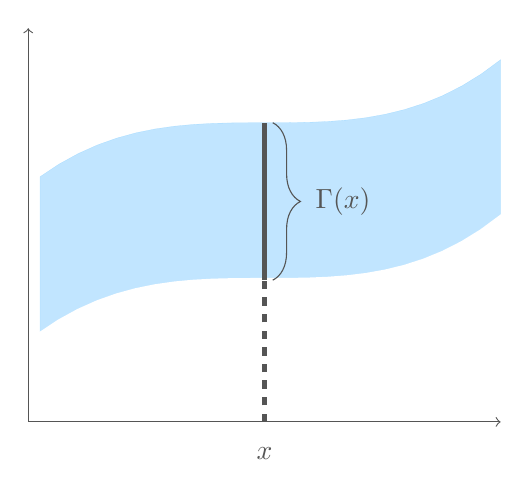
\begin{tikzpicture}[xscale=1.5]
  % Upper bound of region
  \draw[d4blue, ultra thin, domain=0.1:4, fill=d4blue, opacity=0.4] %
    (0.1,0) -- plot (\x, {0.1*pow(\x,3)-0.6*pow(\x,2)+1.2*\x+3}) -- (4,0);

  % Lower bound of region
  \draw[white, ultra thick, domain=0.1:4, fill=white] %
    (0.1,0) -- plot (\x, {0.1*pow(\x,3)-0.6*pow(\x,2)+1.2*\x+1}) -- (4,0);

  % Axis
  \draw[d4black, <->] (0,5) -- (0,0) -- (4,0);

  % Dashed Line at x
  \draw[d4black, ultra thick, dashed, -] %
    (2,0) node[below, yshift=-5pt] {$x$} -- (2,1.8);

  % Vertical \Gamma(x) line
  \draw[d4black, ultra thick, -] (2,1.8) -- (2,3) -- (2,3.8);

  % Brace marking Gamma(x)
  \draw[%
      d4black, decorate, %
      decoration={brace, amplitude=10pt, mirror}, xshift=2pt
    ] %
    (2,1.8) -- (2,3.8) node[midway, right, xshift=12pt] {$\Gamma(x)$};
\end{tikzpicture}
\end{figure}

As shown, numbers in $\R$ on the $x$-axis map into intervals along the
$y$-axis (rather than just a single point as they would for a curve).
An example is shown for one particular $x$.
\end{ex}

\begin{defn}{(Lower Hemi-Continuous)}
Correspondence $\Gamma:X\rightrightarrows Y$ is \emph{lower
hemi-continuous} (LHC) if and only if points don't ``pop up out of
nowhere'' in the limit.

Formally, choose $x\in X$. Note that we require
$\Gamma(x)\neq\emptyset$. Now let $\{x_n\}\subseteq X$ be any arbitrary
sequence converging to $x\in X$. Now choose any $y\in\Gamma(x)$.  For
$\Gamma$ to be LHC at $x$, you need to be able to construct a sequence
\begin{align*}
  \{y_n\}\rightarrow y
  \quad\text{s.t.}\quad
  y_n \in \Gamma(x_n) \quad\forall n
\end{align*}
Now the informal definition makes sense. If $y$ popped up out of
nowhere in the limit, then you could not construct a sequence $\{y_n\}$
converging to it whose elements stayed inside the sets
$\{\Gamma({x_n})\}$ the whole time.
\end{defn}
\begin{figure}[htpb!]
\centering
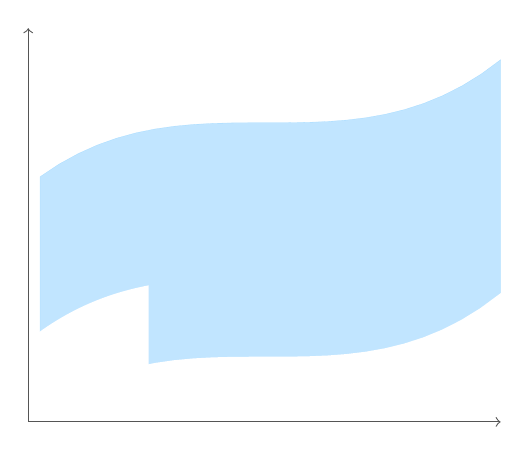
\begin{tikzpicture}[xscale=1.5]
  % Upper bound of region
  \draw[d4blue, ultra thin, domain=0.1:4, fill=d4blue, opacity=0.4] %
    (0.1,0) -- plot (\x, {0.1*pow(\x,3)-0.6*pow(\x,2)+1.2*\x+3}) -- (4,0);

  % Left segment
  \draw[white, ultra thick, domain=0.1:1, fill=white] %
    (0.1,0) -- plot (\x, {0.1*pow(\x,3)-0.6*pow(\x,2)+1.2*\x+1}) -- (1,0);

  % Middle segment
  \draw[white, ultra thick, domain=0.1:4, fill=white] %
    (0.1,0) -- plot (\x, {0.1*pow(\x,3)-0.6*pow(\x,2)+1.2*\x}) -- (4,0);

  %% Lower bound of region
  %\draw[white, ultra thick, domain=0.1:4, fill=white] %
    %(0.1,0) -- plot (\x, {0.1*pow(\x,3)-0.6*pow(\x,2)+1.2*\x+1}) -- (4,0);

  % Axis
  \draw[d4black, <->] (0,5) -- (0,0) -- (4,0);

  %% Dashed Line at x
  %\draw[d4black, ultra thick, dashed, -] %
    %(2,0) node[below, yshift=-5pt] {$x$} -- (2,1.8);

  %% Vertical \Gamma(x) line
  %\draw[d4black, ultra thick, -] (2,1.8) -- (2,3) -- (2,3.8);

  %% Brace marking Gamma(x)
  %\draw[%
      %d4black, decorate, %
      %decoration={brace, amplitude=10pt, mirror}, xshift=2pt
    %] %
    %(2,1.8) -- (2,3.8) node[midway, right, xshift=12pt] {$\Gamma(x)$};
\end{tikzpicture}
\end{figure}

\begin{defn}{(Upper Hemi-Continuous)}
The \emph{compact} correspondence $\Gamma:X\rightrightarrows Y$ is
\emph{upper hemi-continuous} (UHC) if and only if points don't
``disappear'' in the limit.

Formally, choose $x\in X$. Note that we require
$\Gamma(x)\neq\emptyset$. Now let $\{x_n\}\subseteq X$ be any arbitrary
sequence converging to $x$. Also let $\{y_n\}$ be any sequence where
\begin{align*}
  y_n \in \Gamma(x_n) \quad\forall n
\end{align*}
For $\Gamma$ to be UHC at $x$, it must the case that $\{y_n\}$ has a
convergent subsequence that converges to some $y\in \Gamma(x)$.

Now the informal definition makes sense. If there were some $y'\in Y$
such that $y_n = y' \in \Gamma(x_n)$ for all $n$ (implying
$y_n\rightarrow y'$), then we also want $y'\in \Gamma(x)$. It shouldn't
disappear in the limit.
\end{defn}

\begin{defn}{(Continuous Correspondence)}
Compact-valued correspondence $\Gamma:X\rightrightarrows Y$ is
\emph{continuous} at $x\in X$ if it is both UHC and LHC at $x$.
\end{defn}

\subsection{Preliminaries: Theorem of the Maximum}

Next, suppose we want to solve an optimizaton problem of the form
\begin{align*}
  \max_{y\in \Gamma(x)} f(x,y)
\end{align*}
given objective function $f:X\times Y\rightarrow\R$ and correspondence
$\Gamma:X\rightrightarrows Y$ that describes the feasible sets for some
initial condition or parameter, $x\in X$.

\begin{thm}
If $f$ is continuous and $\Gamma$ is continuous and compact-valued, then
\begin{align*}
  y^*(x) = \argmax_{y\in\Gamma(x)} f(x,y)
\end{align*}
is nonempty, compact-valued, and UHC.
\end{thm}

\begin{cor}
If $y^*(x)$ is unique for all $x$, it's just continuous rather than UHC.
\end{cor}

\begin{thm}{\emph{(Theorem of the Maximum)}}
If $f$ is continuous and $\Gamma$ is continuous and compact-valued, then
the function
\begin{align}
  \label{prob:thm-max}
  v(x) = \max_{y\in\Gamma(x)} f(x,y)
\end{align}
is well-defined and continuous.
\end{thm}



\subsection{Canonical Sequential Problem and its Bellman Formulation}


\begin{defn}{(Canonical Sequential Problem)}
We want to solve problems of the form
\begin{align}
  \label{prob:sequential-short}
  \max_{\{x_{t+1}\}_{t=0}^\infty}
  \quad &\sumtinfz \beta^t F(x_t,x_{t+1})\\
  &x_{t+1} \in \Gamma(x_t) \qquad \forall t\notag\\
  &x_0 \; \text{given}\notag
\end{align}
This the \emph{Canonical Sequential Problem}, since the task involves
choosing a sequence $\{(x_{t+1})\}_{t=1}^\infty$ that maximizes the
value of the objective function.
\begin{enumerate}
  \item \emph{State}, $x_t$: At each time $t$, the variable
    $x_t$---called the state---is something like a ``sufficient
    statistic'' for the problem, encoding information about feasible
    sets for $x_{t+1}$ or ``continuation sequences.''
  \item \emph{Control}, $x_{t+1}$: At time $t$, taking the current state
    $x_t$ as given, the agent chooses tomorrow's state $x_{t+1}$
    directly (since this world is deterministic). Since this object is
    chosen and controlled by the agent, $x_{t+1}$ is called the
    \emph{control}.
  \item \emph{Feasibility Constraints}, $\Gamma(x_t)$: The
    correspondence $\Gamma(x_t)$ returns a set of possible values that
    $x_{t+1}$ can take on.
\end{enumerate}
\end{defn}

\begin{defn}{(Alternate Representation: Canonical Sequential Problem)}
\label{defn:sequential-altrep}
For completeness, here's another, perfectly equivalent way the canonical
representation problem might be written. This corresponds to the Sargent
representation.
\begin{align}
  \label{prob:altrep}
  \max_{\{(y_t,x_{t+1})\}_{t=0}^\infty}
  \quad &\sumtinfz \beta^t F(x_t,x_{t+1},y_t)\\
  &x_{t+1} \in \Gamma(x_t,y_t) \qquad \forall t\notag\\
  &x_0 \; \text{given}\notag
\end{align}
Everything is the same except for the introduction of $y_t$ and a slight
change in terminology. Rather than choosing the state $x_{t+1}$ directly
at time $t$ (and calling \emph{that} the control), the agent chooses
$y_t$ at time $t$, which we now call the control in
Problem~\ref{prob:altrep}.  This choice of $y_t$ then influences or
determines the next period's state, $x_{t+1}$, according to some
deterministic law of motion. Of course, the key insight is that we can
always use this deterministic law of motion to write $y_t =
g(x_t,x_{t+1})$ for some deterministic function $g$ and have the agent
choose $x_{t+1}$---dispensing with the need to include $y_t$ at all.

Therefore, I will mostly stick to the representation in
Problem~\ref{prob:sequential-short} throughout this section. It's an
equivalent but more compact way to write these problems, and that seems
desirable for the upcoming proofs.
But I wanted to mention the more verbose representation in
Problem~\ref{prob:altrep} since it's also standard, and since this
representation generalizes most naturally when we go to continuous time
dynamic programming problems in Section~\ref{sec:continuous-dynamic}.
\end{defn}
\begin{note}
Function $F$ and correspondence $\Gamma$ in Problem~\ref{prob:altrep}
are different from that of Problem~\ref{prob:sequential-short}.  I used
identical notation purely for simplicitly.
\end{note}

%\begin{defn}{(Set of Feasible Plans)}
%Given Problem~\ref{prob:sequential-short} and starting value $x_0$,
%define the set of all feasible sequences
%\begin{align*}
  %\Pi(x_0)
  %&:= \{ \{x_{t+1}\}^\infty_{t=0} \; | \;
  %x_{t+1}\in \Gamma(x_t) \; \forall t, \; x_0 \,\text{given}\}
%\end{align*}
%Therefore, a plan or sequence $\tilde{x}:=\{x_{t+1}\}_{t=0}^\infty$ is
%feasible for Problem~\ref{prob:sequential-short} if
%$\tilde{x}\in\Pi(x_0)$, implying that is satisfies all feasibility
%constraints.
%\end{defn}

\begin{defn}{(Bellman Equation Formulation and Value Function)}
\label{defn:bellman}
Suppose that we face Problem~\ref{prob:sequential-short}.  Also suppose
that we have access to a function $v_B(x_0)$ called the \emph{value
function} that returns the value of the objective function in
Problem~\ref{prob:sequential-short} \emph{after} maximizing over the set
of all feasible plans for starting point $x_0$. (We'll prove that such a
function does exist later. For now, just take it as given.) This
function can be written
\begin{align*}
  v_B(x_0) :=
  \max_{\{x_{t+1}\}^\infty_{t=1}}\;
  \sumtinfz \beta^t F(x_t,x_{t+1})
  \qquad x_{t+1}\in\Gamma(x_t)\;\forall t
\end{align*}
But this can instead be written recursively as
\begin{align*}
  v_B(x_0)
  %&=
  %\max_{\{x_{t+1}\}^\infty_{t=1}}\;
  %F(x,x_1) +
  %\sum^\infty_{t=1} \beta^t F(x_t,x_{t+1})\\
  &=
  \max_{\{x_{t+1}\}^\infty_{t=1}}\;
  F(x_0,x_1) +
  \beta \sum^\infty_{t=0} \beta^{t+1} F(x_{t+1},x_{t+2})\\
  \Leftrightarrow\qquad
  &=
  \max_{x_1\in\Gamma(x_0)}\;
  F(x_0,x_1) +
  \beta v_B(x_1)
\end{align*}
Generalizing notation a bit, we have what's called the \emph{Bellman
Equation}
\begin{align}
  \label{eq:vB}
  v_B(y) &=
  \max_{y\in\Gamma(x)}\;
  F(x,y) +
  \beta v_B(y)
\end{align}
This formulation exploits the symmetry of the problem over time to
produce a recursive representation.  Given today's starting value $x$,
rather than choose an infinite sequence $\{x_{t+1}\}_{t=0}^\infty$, I
need only choose tomorrow's starting value $y$.  Since the value
function tells me how much the starting value $y$ is worth, I can frame
the problem as a tradeoff between $F(x,y)$ today and the discounted
value of tomorrow's $v_B(y)$.

So we've amazingly turned an infinite-dimensional sequential problem of
finding $\{x_{t+1}\}^\infty_{t=0}$ into something much simpler, provided
that $v_B$ exists (we'll still have to prove it does).  That means
solving Functional Equation~\ref{eq:vB} for fixed point $v_B$. Then,
once we have $v_B$, we can think about determining the optimal sequence.
\end{defn}

\begin{defn}{(Optimal Value)}
\label{defn:vstar}
Given Problem~\ref{prob:sequential-short}, define the optimal value as
\begin{align}
  v^*(x_0) := \sup_{\{x_{t+1}\}_{t=0}^\infty}
  \; &\sumtinfz \beta^t F(x_t,x_{t+1})
  \qquad \text{where}\;
  \forall t, \; x_{t+1} \in \Gamma(x_t)
\end{align}
Note that I changed the max to a sup since the latter always exists, so
this is well-defined. That's in stark contrast to $v_B$ in the Bellman
Equation formulation, which was merely assumed to exist and also implied
existence of a feasible plan $\{x_t\}_{t=0}^\infty$ that maximized the
objective function. Now we'll show under what conditions $v^*$ and $v_B$
are equal---i.e.\ the conditions under which the optimal value is
obtained.
\end{defn}

\subsection{Principal of Optimality: Equivalence of Sequential and
Bellman Formulations}

In this section we look at conditions under which the optimal value
function $v^*$ is also the function $v_B$ satisfying the Bellman
Equation, and vice versa.

\begin{assump}{(Nonempty Feasible Sets)}
\label{assump:feasible}
$\Gamma(x)\neq\emptyset$ for all $x\in X$, so we can always find a
feasible sequence given any starting point.
\end{assump}

\begin{assump}{(Finite Objective Function)}
\label{assump:finite}
For all feasible sequences $\{x_{t+1}\}_{t=0}^\infty$ such that
$x_{t+1}\in \Gamma(x_t)$ for all $t$, we have
\begin{align*}
  \lim_{T\rightarrow\infty} \sum_{t=0}^T \beta^t F(x_t,x_{t+1})
  < \infty
\end{align*}
Note, this is assured if $F(x,y)$ is a bounded function and
$\beta\in[0,1)$.
\end{assump}

\begin{thm}
\label{thm:vstar-solves-bellman}
Given Problem~\ref{prob:sequential-short}, if
Assumptions~\ref{assump:feasible} and~\ref{assump:finite} hold, then
$v^*$ from Definition~\ref{defn:vstar} satisfies the Bellman Equation
\begin{align}
  \label{vstar-solves-bellman}
  v^*(x) = \sup_{y\in\Gamma(x)} F(x,y) + \beta v^*(y)
\end{align}
\end{thm}
\begin{proof}
For arbitrary $x\in X$, we want to show that the value $v^*(x)$ equals
the RHS of Equation~\ref{vstar-solves-bellman}---i.e.\ that it is indeed
the RHS sup. By the definition of sup, that's true if and only if
\begin{enumerate}
  \item[A1.] $v^*(x) \geq F(x,y) + \beta v^*(y)$ for all $y\in\Gamma(x)$.
  \item[A2.] For any $\varepsilon>0$, we can find a
    $y_\varepsilon\in\Gamma(x)$ such that
    $
      v^*(x) < F(x,y_\varepsilon) + \beta v^*(y_\varepsilon) + \varepsilon
    $
\end{enumerate}
That's what we need to show. Now onto what we know.
Specifically, we know that $v^*$ is the sup over the sequential problem
as defined in Definition~\ref{defn:vstar}. So again, by the definition
of the sup, we know that
\begin{enumerate}
  \item[B1.] $v^*(x) \geq \sumtinfz \beta^t F(x_t,x_{t+1})$ for all
    feasible sequences satisfying $x_{t+1}\in\Gamma(x_t)$ with starting
    value $x_0=x$.
  \item[B2.] For any $\varepsilon>0$, there exists feasible
    $\{\tilde{x}_{t+1}\}_{t=0}^\infty$ such that
      $
      v^*(x) < \sumtinfz \beta^t
      F(\tilde{x}_{t}, \tilde{x}_{t+1}) + \varepsilon
      $
      with starting value $x_0=x$.
\end{enumerate}
Our task is to show that (B1) and (B2) together imply (A1) and (A2).

(Show A1) Let $x_0$ and $\varepsilon>0$ be given.
Let $x_1$ be any point in $\Gamma(x_0)$. Then by (B2)
and some index renumbering, there exists a feasible sequence
$\{x_{t+2}\}_{t=0}^\infty$ such that
\begin{align}
  v^*(x_1) &< \sumtinfz \beta^t
  F(x_{t+1}, x_{t+2}) + \varepsilon \notag \\
  \Leftrightarrow\quad
  v^*(x_1) - \varepsilon &< \sumtinfz \beta^t
  F(x_{t+1}, x_{t+2})
  \label{seqchoice}
\end{align}
Onto this just-chosen sequence, prepend
$x_1\in\Gamma(x_0)$ so we now have sequence
$\{x_{t+1}\}_{t=0}^\infty$. All elements were chosen to be
feasible.  So by (B1), we know that for feasible sequence
$\{x_{t+1}\}_{t=0}^\infty$
\begin{align*}
  v^*(x_0)
  &\geq \lim_{T\rightarrow\infty} \sumtTz \beta^t F(x_t,x_{t+1}) \\
  \text{Pop off first element} \qquad
  &= F(x_0, x_1) + \lim_{T\rightarrow\infty} \sumtT \beta^t F(x_t,x_{t+1}) \\
  \text{Renumbering indices} \qquad
  &= F(x_0, x_1) + \beta \lim_{T\rightarrow\infty} \sumtTz \beta^{t} F(x_{t+1},x_{t+2}) \\
  \text{By Inequality~\ref{seqchoice}} \qquad
  &= F(x_0, x_1)
  + \beta \left[ v^*(x_1) - \varepsilon\right]
\end{align*}
Since $\varepsilon>0$, starting point $x_0$, and
$x_1\in\Gamma(x_0)$ were arbitrary
\begin{align*}
  v^*(x_0)
  &\geq F(x_0, x_1)
  + \beta  v^*(x_1)
\end{align*}
which is the same as (A1), provided you replace $x_0$ and $x_1$ with $x$
and $y$.

(Show A2)
Suppose that $x$ and $\varepsilon>0$ are given.
By (B2), there exists a feasible sequence with $x_0=x$ such that
\begin{align*}
  v^*(x) &< \lim_{T\rightarrow\infty} \sumtTz \beta^t
  F(x_{t}, x_{t+1}) + \varepsilon \\
  \Leftrightarrow\quad
  v^*(x) &< F(x, x_1)
  + \lim_{T\rightarrow\infty}
  \sumtT \beta^t
  F(x_{t}, x_{t+1}) + \varepsilon \\
  \Rightarrow\quad
  v^*(x) &< F(x, x_1)
  + \beta v^*(x_1)
  + \varepsilon \\
\end{align*}
Note, we were able to replace the series $\sumtT \beta^t F(x_{t},
x_{t+1})$ with $\beta v^*(x_1)$ by using B1.
So now, just choose $y=x_1$. We know $x_1\in\Gamma(x_0)$ is feasible
and $x_0=x$. This means A2 holds.
\end{proof}

Now we move onto the other direction: Does a function $v_B$ satisfying
the Bellman Formulation also match the optimal value function $v^*$. For
that, we need one additional assumption beyond
Assumptions~\ref{assump:feasible} and~\ref{assump:finite} that we made
before.

\begin{assump}{(Transversality Condition)}
\label{assump:transversality}
For value function $v$ and all feasible sequences
$\{x_{t+1}\}_{t=0}^\infty$ such that $x_{t+1}\in \Gamma(x_t)$ for all
$t$, we have
\begin{align*}
  \lim_{t\rightarrow\infty} \beta^t v(x_t) = 0
\end{align*}
In words, ``The value of stuff in the infinite future doesn't matter.''
\end{assump}

\begin{thm}
Given Problem~\ref{prob:sequential-short}, suppose
Assumptions~\ref{assump:feasible},~\ref{assump:finite},
and~\ref{assump:transversality} hold and that function $v_B$ satisfies
Bellman Equation
\begin{align}
  \label{eq:bellmansup}
  v_B(x) = \sup_{y\in\Gamma(x)} F(x,y) + \beta v_B(y)
\end{align}
Then $v_B = v^*$, the optimal value function for the sequential problem,
which was defined in Definition~\ref{defn:vstar}.
\end{thm}
\begin{rmk}
Though the Bellman formulation above used max rather than sup, I use sup
here so I don't have to worry about existence.
\end{rmk}
\begin{proof}
%In this proof, I'll be using statements similar to A1, A2, B1, and B2
%from the proof of Theorem~\ref{thm:vstar-solves-bellman}. So let's
%restate them appropriately for this problem.

For arbitrary $x\in X$, we want to show that $v_B(x)=v^*(x)$, with the
latter representing the optimal value---the supremum over all sequences.
That only occurs if
\begin{enumerate}
  \item[A1.] $v_B(x) \geq \sumtinfz \beta^t F(x_t,x_{t+1})$ for all
    feasible sequences satisfying $x_{t+1}\in\Gamma(x_t)$ with starting
    value $x_0=x$.
  \item[A2.] For any $\varepsilon>0$, there exists feasible
    $\{\tilde{x}_{t+1}\}_{t=0}^\infty$ such that
      $
      v_B(x) < \sumtinfz \beta^t
      F(\tilde{x}_{t}, \tilde{x}_{t+1}) + \varepsilon
      $
      with starting value $x_0=x$.
\end{enumerate}
That's what we need to show. Now onto what we know.  Specifically, we
know that $v_B$ solves the Bellman Equation, so it equals the RHS of
Equation~\ref{eq:bellmansup}. Since it's a supremum, by definition
\begin{enumerate}
  \item[B1.] $v_B(x) \geq F(x,y) + \beta v_B(y)$ for all $y\in\Gamma(x)$.
  \item[B2.] For any $\varepsilon>0$, we can find a
    $y_\varepsilon\in\Gamma(x)$ such that
    $
      v_B(x) < F(x,y_\varepsilon) + \beta v_B(y_\varepsilon) + \varepsilon
    $
\end{enumerate}
Our task is to show that (B1) and (B2) together imply (A1) and (A2).

(Show A1) Let $\{x_{t+1}\}_{t=0}^\infty$ be a feasible sequence. We can
use B1 to recursively substitute:
\begin{align*}
  v_B(x) &\geq F(x,x_1) + \beta v_B(x_1) \\
  v_B(x) &\geq F(x,x_1) + \beta F(x_1, x_2) + \beta^2 v_B(x_2) \\
  \vdots \quad & \quad \qquad \vdots \\
  v_B(x) &\geq \sumtTz \beta^t F(x_t,x_{t+1}) + \beta^{T+1} v_B(x_{T+1}) \\
  \lim_{T\rightarrow\infty}
  v_B(x) &\geq
    \lim_{T\rightarrow\infty}
    \left\{
    \sumtTz \beta^t F(x_t,x_{t+1}) + \beta^{T+1} v_B(x_{T+1})
    \right\}\\
  v_B(x) &\geq
    \sumtinfz \beta^t F(x_t,x_{t+1})
    + 0
\end{align*}
Where we needed Assumption~\ref{assump:transversality} on transversality
to ensure that the term $\beta^{T+1}v(x_{T+1})$ goes to zero.

(Show A2) Next,
\end{proof}

\begin{ex}{(Why We Need Transversality)}
In this example, we set up a problem whose Bellman Equation formulation
has a solution, while the sequential problem has no optimal value
function solution. Now onto the problem.

Consider a simple consumption/investment decision:
\begin{align*}
  \max_{\{c_t\}_0^\infty} \; &\sumtinfz \beta^t c_t \\
  & c_t + a_{t+1} = (1+r)a_t\\
  & c_t \geq 0
\end{align*}
where $a_0$ is given as initial endowment. We can express this problem
in standard form with $a_t$ as the state variable
\begin{align*}
  \max_{\{a_{t+1}\}_0^\infty} \;
  &\sumtinfz \; \beta^t [(1+r)a_t - a_{t+1}] \\
  & (1+r)a_t - a_{t+1} \geq 0
\end{align*}
where $F(a_t,a_{t+1}) = (1+r)a_t - a_{t+1}$.
We place \emph{no restrictions} on each $a_t$---they can be arbitrarily
negative, and that will be important.
Under some assumptions $1+r = \frac{1}{\beta}$.

So now we can write the Bellman Equation formulation:
\begin{align*}
  v(a) = \max_{a'} \; \left(\frac{a}{\beta} - a'\right) + \beta \, v(a')
\end{align*}
Now we use the guess and verify method. The guess is $v(a) = a/\beta$.
\begin{align*}
  \text{Check} \qquad
  \frac{a}{\beta}
  &= \max_{a'} \;
  \left(\frac{a}{\beta} - a'\right)
  + \beta \left(\frac{a'}{\beta}\right)\\
  \frac{a}{\beta}
  &= \max_{a'} \;
  \frac{a}{\beta}
  =
  \frac{a}{\beta}
\end{align*}
So this solves the Bellman Equation.

Time to see why this won't work. Pick initial consumption $c_0$ to be
\emph{huge}. That is, borrow a lot so you consume a lot in the first
period, consuming $c_0 >> a_0$.
Thereafter, consume nothing: $c_t=0$ for $t>0$. This results in an
investment profile of
\begin{align*}
  a_{1} &= \frac{a_0}{\beta} - c_0 < 0 \\
  \Rightarrow \quad
  a_{t+1} &= \frac{a_t}{\beta}
  = \frac{a_0}{\beta^{t+1}} - \frac{c_0}{\beta^t}
\end{align*}
Since $a_1$ is negative and $\beta<1$, we see that $a_{t+1}$ will blow
up to negative infinity.
Now in each period, $a_{t+1}$ is a finite, very negative, but
still-feasible number since we didn't put any borrowing constraints on.
And that's exactly the problem. The agent could go on borrowing forever.

Let's now make the violation of the transversality condition more
explicit, checking the limit in Assumption~\ref{assump:transversality}.
To simplify the math, let $a_0=0$. Recall that $v(a) = a/\beta$.
\begin{align*}
  \lim_{t\rightarrow\infty} \beta^t v(a_t)
  = \lim_{t\rightarrow\infty} \beta^t \left(\frac{a_t}{\beta}\right)
  = \lim_{t\rightarrow\infty} \beta^t
  \left(
  \frac{-c_0/\beta^{t-1}}{\beta}
  \right)
  = \lim_{t\rightarrow\infty}
  -c_0
  = -c_0 \neq 0
\end{align*}
In other words, the value function is not ``small'' in the infinite
future.

So in summary, there is no optimal value function $v^*$, though we were
able to find a function satisfying the Bellman equation. In general,
only checking the transversality condition catches this kind of problem.
\end{ex}


\subsection{Bellman Operator}

How do you actually go about solving a Bellman Equation? In this
section, we describe the Bellman Operator and some results about it
which answer that question.

\begin{defn}
Define the Bellman operator
$T:\mathscr{B}(X,\R)\rightarrow\mathscr{B}(X,\R)$
acting on the set of bounded real-valued functions as
\begin{align*}
  T[v(x)]
  &= \sup_{y\in\Gamma(x)}
  F(x,y) + \beta v(y)
\end{align*}
This takes in a function $v$ and spits out another function of $x$.
\end{defn}

\begin{prop}{\emph{(Bellman Operator is a Contraction Map)}}
\end{prop}


\subsection{Solving by Guess and Verify}

Suppose that we have Bellman Equation
\begin{align*}
  v(x) = \max_{y\in\Gamma(x)} F(x,y) + \beta v(y)
\end{align*}
The method of ``guess and verify'' involves choosing some function $v$,
substituting it into the RHS and maximizing the RHS over all feasible
$y\in\Gamma(x)$. The result is a function, and you check that it is
identical to the original $v$ on the LHS.

Often, everything is differentiable, so this means differentiate the
RHS, set equal to zero, solve for $y$, plug in the result, and check
\begin{align*}
  0 &= \frac{\partial}{\partial y}
  \left[
    F(x,y) + \beta\, v(y)
  \right] \\
  \text{Solve for $y$}
  \quad \qquad \;
  0 &= F_y(x,y) + \beta \, v_y(x) \\
  \text{Plug in result $y^*$ and check} \qquad
  v(x) &= F(x,y^*) + \beta\, v(y^*)
\end{align*}

\begin{ex}
Suppose that we face problem
\begin{align*}
  v(k) = \max_{k'\in[0,f(k)]} u(f(k)-k') + \beta\, v(k')
\end{align*}
where $u=\log(c)$ and $f(k)=k^\alpha$.

First step: divine inspiration says guess $v(k) = a + b \; \log(k)$ for
some constants $a$ and $b$ that we'll pin down later.
Now, differentiate the RHS:
\begin{align*}
  \frac{\partial}{\partial k'}
  \left[
  u(f(k)-k') + \beta\, v(k')
  \right]
  &=
  \frac{\partial}{\partial k'}
  \left[
    \log\left(
    k^\alpha - k'
    \right)
    + \beta (a + b\, \log(k'))
  \right] \\
  &= -\frac{1}{k^\alpha-k'}
  + \frac{b\beta}{k'}
\end{align*}
Set that equal to zero and solve for $k'$
\begin{align*}
  0
  &= -\frac{1}{k^\alpha-k'}
  + \frac{b\beta}{k'}\\
  \Rightarrow\quad
  k' &= \frac{b\beta}{1+b\beta} k^\alpha
\end{align*}
Now substitute this into the RHS, and try to work it into something that
looks like $v(k) = a + b\,\log(k)$:
\begin{align*}
  RHS = u(f(k)-k') + \beta \, v(k')
  &=
  \log\left(
    k^\alpha - \frac{b\beta}{1+b\beta} k^\alpha
  \right)
  + \beta
    \left[
      a + b\,\log\left(\frac{b\beta}{1+b\beta} k^\alpha\right)
    \right] \\
  &=
  \log\left(
    \frac{k^\alpha}{1+b\beta}
  \right)
  + a\beta + b\beta\,\log\left(\frac{b\beta}{1+b\beta} k^\alpha\right) \\
  &=
  [a\beta
  + b\beta\,\log\left(b\beta\right)
  - (1+b\beta)\log\left( 1+b\beta \right)]
  +\alpha(1+b\beta)\log\left( k \right)
\end{align*}
Bit of a monster, but we have isolated a bunch of constants and a
constant times $\log k$. We just need to match up constants, so start
with the coefficient on $\log k$:
\begin{align*}
  b\log(k)
  &= \alpha(1+b\beta) \log(k) \\
  \Rightarrow\quad
  b &= \frac{\alpha}{1-\alpha \beta}
\end{align*}
Next, match up the constants to $a$ and solve for $a$ (leaving $b$ as
is):
\begin{align*}
  a
  &=
  a\beta + b\beta\,\log\left(b\beta\right)
  - (1+b\beta)\log\left( 1+b\beta \right) \\
  \Rightarrow\qquad
  a
  &=
  \frac{1}{1-\beta}
  \left[
    b\beta\,\log\left(b\beta\right)
  - (1+b\beta)\log\left( 1+b\beta \right) \right]\\
\end{align*}
For this choice of constants, $v(k) = a + b\,\log(k)$ solves the Bellman
Equation.
\end{ex}

\clearpage
\section{Continuous-Time Deterministic Dynamic Programming}
\label{sec:continuous-dynamic}

In this section, we extend the work of
Section~\ref{sec:discrete-dynamic} on discrete-time dynamic programming
into continuous time. In practice, that means sums become integrals and
difference equations become \emph{differential} equations.  The
formulation we generalize is Problem~\ref{prob:altrep} rather than the
equivalent and more compact Problem~\ref{prob:sequential-short}.

\subsection{Canonical Problem and the Hamiltonian}

Give some objective function $F(x,y,t)$, we want to choose functions
of time, $x_t$ and $y_t$, to solve
%of time, $x_t$ with range $\Rn$ and $y_t$ with range $\R^k$, to solve
\begin{align}
  \max_{x_t,y_t} \; W(x_t,y_t) &=
  \max_{x_t,y_t} \; \int^{T}_{0} F(x_t,y_t,t) \; dt
  \label{prob:cts-dynamic} \\\notag\\
  \text{s.t.} \;
   \dot{x}_t &= G(x_t,y_t,t) \notag \\
  %& y_t \in Y_t \subseteq \R^k \quad \forall t\notag \\
   y_t &\in Y_t \quad \forall t\notag \\
   x_0  &\;\text{given} \notag
\end{align}
We will consider problems where the terminal time $T$ is finite and
where it is infinite.
Again, the key features of this problem are
\begin{enumerate}
  \item \emph{State}, $x_t$:
    %A ``sufficient statistic'' encoding information about feasible sets.
    Its evolution is summarized by a differential equation, where
    $\dot{x}_t := \frac{\partial x_t}{\partial t}$. The evolution of the
    state is influenced by the current state, the choice of control, and
    time.
  \item \emph{Control}, $y_t$: Chosen by the agent in response to the
    state $x_t$. This influences the evolution of the state in the
    future.
  \item \emph{Feasibility Constraints}, $y_t\in Y_t$: At each time
    period, there is some feasible set $Y_t$ in $\R$ or $\Rk$ (if there
    are multiple control variables). We require the choice of control
    $y_t$ lies in $Y_t$ at each period.
  \item \emph{Admissable Pair}, $(x_t,y_t)$: The pair of functions
    $(x_t,y_t)$ is called an admissable pair if they satisfy both
    $\dot{x}_t = G(x_t,y_t,t)$ and $y_t\in Y_t$ for all $t$.
\end{enumerate}

\begin{defn}{(Hamiltonian)}
Given Problem~\ref{prob:cts-dynamic}, define the \emph{Hamiltonian}
\begin{align*}
  H(x,y,\lambda,t) := F(x_t,y_t,t) + \lambda_t G(x_t,y_t,t)
\end{align*}
where $\lambda_t$ is a function called the \emph{co-state}.
This is very much like the static-optimizaton Lagrangian, only now,
we're doing dynamic optimization that involves more than one time
period.
\end{defn}

\begin{defn}{(Necessary Conditions)}
Suppose that we are faced with Problem~\ref{prob:cts-dynamic} where
$T<\infty$ and $F$ and $G$ are continuously differentiable functions.
Suppose that the problem has an interior continuous solution
$y_t$---i.e.\ $y_t$ is continuous and $y_t\in \text{int} \, Y_t$ for all
$t$---with corresponding state variable $x_t$ such that $W(x_t,y_t) \geq
W(\hat{x}_t,\hat{y}_t)$ for all admissable pairs
$(\hat{x}_t,\hat{y}_t)$.\footnote{%
The assumptions that $y$ is an ``interior continuous function''
eliminates the possibility that $y$ is a corner case or discontinuous.
}

Then there exists a continuously differentiable co-state function
$\lambda_t$ such that $(y_t,x_t,\lambda_t)$ satisfy the following
necessary conditions:
\begin{enumerate}
  \item $H_y (x_t,y_t,\lambda_t,t) = 0$
  \item $\dot{\lambda}_t = - H_x(x_t, y_t, \lambda_t, t)$
  \item $\dot{x}_t = H_\lambda(x_t,y_t,\lambda_t,t) = G(x_t, y_t, t)$
  \item $x_0=x_0$ given
  \item $\lambda_T=0$
\end{enumerate}
for all $t\in[0,T]$.
\end{defn}
\begin{rmk}
In the ``proof,'' we will look for the necessary conditions of an
optimal solution by using the \emph{variational principle} of the
calculus of variations.  This will work by assuming that we have an
optimal solution, perturbing that supposedly-optimal solution by small
amounts to get a family of new candidate solutions, and seeing what
necessary conditions we need to place on the original supposedly-optimal
solution so that none of the new candidate solution are any better.

Given that description, it's maybe not surprising that the necessary
conditions are for a \emph{local} optimum rather than a global optimum.
We're simply specifying necessary conditions on some solution $y_t$ that
will rule out better solutions in the neighborhood of $y_t$. We saw a
similar result in the KKT section. But also as in the KKT conditions, a
few extra conditions having to do with convexity can guarantee the
solution is globablly optimal.
\end{rmk}

\begin{proof}{(Kinda)}
Let $y_t$ represent the assumed interior continuous solution, with $x_t$
representing the corresponding state variable. The pair $(y_t,x_t)$ is
assumed optimal so that $W(x_t,y_t) \geq W(\hat{x}_t,\hat{y}_t)$ for all
admissable pairs $(\hat{x}_t,\hat{y}_t)$.

(Construct the Variations)
To generate a family of other ``nearby'' continuous solutions, choose
and fix a continuous function $\eta_t$ and define
\begin{align*}
  y_t(\varepsilon) := y_t + \varepsilon\eta_t
\end{align*}
\end{proof}
For each fixed $\varepsilon$, the \emph{variation} $y_t(\varepsilon)$ is
a continuous function. By varying $\varepsilon$, we generate a
\emph{family} of continuous variations. Given each variation of the
control $y_t(\varepsilon)$, define corresponding $x_t(\varepsilon)$
satisfying
\begin{align}
  \dot{x}_t(\varepsilon)
  = G(x_t(\varepsilon), y_t(\varepsilon), t)
  \qquad x_0(\varepsilon)=x_0
  \label{xvardef}
\end{align}
Given admissable pair $(x_t(\varepsilon), y_t(\varepsilon))$, let's also
define
\begin{align}
  W(\varepsilon) := W(x_t(\varepsilon), y_t(\varepsilon))
  = \int^{T}_0 F(x_t(\varepsilon), y_t(\varepsilon), t) \, dt
  &\underbrace{\leq W(0)} \label{Weps} \\
  &\;\text{Since $(x_t,y_t)$ optimal}
  \notag
\end{align}
Lastly, to ensure feasibility of the variations, note that for fixed
$\eta_t$, the function is continuous on a compact interval, hence
$\eta_t$ is bounded.  Therefore, you can always choose an
$\varepsilon_\eta$ such that
\begin{align*}
  |\varepsilon| < \varepsilon_\eta
  \implies
  y_t(\varepsilon) \in \text{int} \, Y_t \quad\forall t
\end{align*}
For the reasons mentioned in the remark about, this restriction to
variations with $\varepsilon<\varepsilon_\eta$ is not a problem.

Now that we have this family of variations, let's derives the necessary
conditions we need to put on $y_t$ so that none of the
$y_t(\varepsilon)$ are better.

(Prove the Conditions)
By definition of Equation~\ref{xvardef}
\begin{alignat}{3}
  0 &= G(x_t(\varepsilon), y_t(\varepsilon), t) - \dot{x}_t(\varepsilon)
  &&\forall t\in[0,T] \notag \\
  \Rightarrow \quad
  0 &= \int^{T}_0
  \lambda_t \; [
    G(x_t(\varepsilon), y_t(\varepsilon), t) -
    \dot{x}_t(\varepsilon)
  ] \, dt
  \qquad&&\forall \lambda_t:[0,T]\rightarrow \R
  \label{lambdadef}
\end{alignat}
where $\lambda_t$ is any function. Assume it is continuously
differentiable.\footnote{%
Did I cool you down with that hand wave. I'm just going to assume that
for now.}
If we choose it correctly (with a few conditions on the function), it
will be called the \emph{co-state} and will behave like a Lagrange
multiplier.

Now do the following addition
\begin{align*}
  W(\varepsilon) &= W(\varepsilon) + 0
  = W(\varepsilon) +\text{(RHS of \ref{lambdadef})} \\
  \Rightarrow \quad
  W(\varepsilon) &=
  \int^{t_1}_0
  \left\{
  F(x_t(\varepsilon), y_t(\varepsilon), t)
  + \lambda_t [
    G(x_t(\varepsilon), y_t(\varepsilon), t) -
    \dot{x}_t(\varepsilon)
  ]
  \right\}\, dt
\end{align*}
Integrating the $\int \lambda_t \dot{x}_t(\varepsilon)$ by parts to turn
the $\lambda$ into $\dot{\lambda}$ and $x$ into $\dot{x}$, you get
\begin{align*}
  \int^{t_1}_0 \lambda_t \dot{x}_t(\varepsilon) \, dt
\end{align*}

\end{document}


%Suppose that an infinitely-lived agent gets utility in period $t$ from
%consuming $y_t$. The variable $y_t$ is called the \emph{control}; its
%value is chosen by the agent at time $t$ given some pre-determined
%value, $x_t$, called the \emph{state}.  Between periods, the future
%state $x_{t+1}$ is a deterministic function of $x_t$ and $y_t$, i.e.
%\begin{align}
  %\label{xevol}
  %x_{t+1} = g(x_t, y_t)
  %\qquad
  %\text{$x_0$ given}
%\end{align}
%Typically, the function $g$ will involve some tradeoff between $y_t$ and
%$x_{t+1}$. For example, given $x_t$, the more $y_t$ (perhaps
%consumption) an agent chooses today, the less $x_{t+1}$ he gets next
%period (perhaps capital from investment).

%Next, our problem is to maximize discounted lifetime utility:
%\begin{align}
  %\label{toughproblem}
  %\sum^\infty_{t=0} \beta^t u(y_t)
  %\qquad \beta\in (0,1)
%\end{align}
%by choosing a feasible and optimal path $\{ y_t \}_0^\infty$, again
%subject to an initial condition $x_0$.  Here,
%``optimal'' means utility maximizing. Typically, feasibility
%will be determined by some sort of resource constraint
%(such as $y_t\leq x_t$ or $y_t\leq f(x_t)$) or some
%restriction to non-negativity of the sequence(s) $\{ y_t
%\}$ and/or $\{x_t\}$.

%To make things simpler, we will now define a bit of
%notation for feasibility. At time $t$, the set of all
%feasible $y_t$ is denoted $\mathcal{F}_t$. Therefore, $y_t$
%is feasible if $y_t\in \mathcal{F}_t$. More generally, a
%sequence $\{y_t\}^\infty_0$, abbreviated $\{y_t\}$, is
%feasible if $\{y_t\} \subset \mathcal{F}$.


%\subsection{Value Function and Bellman Equation}

%For reasons that we'll see soon, we'll want to define the
%Bellman Equation for our optimization problem. That first
%entails defining the value function, $v^*$:
%\begin{align*}
  %v^*(x_0) = \sup_{ \{y_t\} \subset \mathcal{F}}
  %\sum^\infty_{t=0} \beta^t u(y_t)\;
  %\qquad
  %\text{$x_0$ given}
%\end{align*}
%In words, the value function $v^*(x_0)$ describes that
%maximum discounted value that can be obtained from initial
%state $x_0$.

%With the value function defined, we can now write the
%Bellman Equation, which looks very similar to what we had
%for the Shortest Path problem described above:
%\begin{align}
  %v^*(x_t) &= \max_{y_t \in \mathcal{F}_t}
  %\left\{ u(y_t) + \beta \; v^*\big(g(x_t, y_t)\big) \right\} \\
    %\text{By (} \quad \Leftrightarrow \quad
  %&= \max_{y_t \in \mathcal{F}_t}
    %\left\{ u(y_t) + \beta v^*(x_{t+1}) \right\} \notag
%\end{align}
%Intuitively, this equation says that you maximize the value from the
%current state, $x_t$, by trading off current reward, $u(y_t)$, in
%exchange for the discounted future value of the resulting state,
%$\beta v^*(x_{t+1})$.

%Since we've formulated the problem in Bellman terms, it's
%clear that we'll eventually want to apply dynamic
%programming methods to solve for the value function $v^*$.
%That's what we did in the Shortest Path problem above; it's
%likely what we'll want to do again.


%\emph{However}, solving for the value function $v^*$ above
%doesn't \emph{quite} give us what we want. We don't just
%want to know the maximum lifetime utility of an agent; we
%want to know what path they will choose for the control.
%In other words, we want to know $\{y_t\}_0^\infty$.

%To solve for this sequence, we now discuss the policy function approach,
%which allows us to answer this question while also redefining the
%motivating problem and the Bellman Equation in simpler, more practical
%terms.


%\subsection{The Policy Function Approach}

%To start, note that even if we can solve for the value function,
%$v^*(x_0)$ (and we can't yet), our real goal of directly specifying the
%optimal path $\{y_t\}_0^\infty$ is hard. It amounts to selecting a point
%in infinite-dimensional space.  So we'll do something easier.
%Specifically, we'll seek a \emph{policy function}---some function or
%``decision rule'' $\sigma$ that depends only upon the current state such
%that
%\begin{align}
  %\label{markov}
  %y_t = \sigma(x_t) = \sigma(g(x_{t-1}, y_{t-1}))
  %\qquad \sigma \in \Sigma
%\end{align}
%where $\Sigma$ is the set of all feasible policies. So rather than
%trying to say \emph{what} an agent will choose, we'll describe
%\emph{how} that agent will choose.

%Now a well-known result from dynamic programming says that, in the types
%of problems we want to consider, an optimal consumption sequence must be
%Markov just as in Equation \ref{markov} above, so that a policy function
%$\sigma$ will, indeed, exist.  This function $\sigma$ will also be
%time-homogeneous, so it will remain the same for all $t$.  This is all
%just to say that we're doing something reasonable that will allow us to
%find the optimal path $\{y_t\}$.

%\subsubsection{Adapting the Problem and Objective}

%So first, we can rewrite our motivating problem as
%expressed in () and () in
%terms of the policy function:
%\begin{align}
  %\label{policyapproach}
  %\max_{\sigma \in \Sigma}
  %&\left\{ \sum^\infty_{t=0} \beta^t u(\sigma(x_t)) \right\}\\
  %\text{where} &\quad
  %x_{t+1} = g(x_t, \sigma(x_t))
  %\qquad \text{$x_0$ given}
  %\notag
%\end{align}
%Since $g$ is assumed deterministic, we see that the only
%unknown in the problem written above is the policy
%function, $\sigma$. We have everything else we need.

%This is the crux of the policy function approach.
%Rather than having our unknown be a utility-maximizing
%infinite sequence $\{y_t\}^\infty_0$, we find a single
%function $\sigma$ that provides a map or decision rule to
%go from the state ($x_t$) to the optimal choice for the
%control ($y_t$).  This choice then propagates to the next
%period via deterministic $g$ to define the state next
%period.

%\subsubsection{Adapting the Value Function}

%Now that we've translated the basic problem into policy
%function terms, let's see what that means for the value
%function and Bellman equation we defined above.

%So first, for each feasible policy $\sigma\in
%\Sigma$, define a \emph{policy value
%function}: \begin{align*}
  %v_\sigma(x_0) :=
  %\left\{ \sum^\infty_{t=0} \beta^t u(\sigma(x_t)) \right\}
%\end{align*}
%This gives the utility conditional on a policy and an initial
%condition.  Our goal will be to choose an \emph{optimal} policy,
%i.e. a policy function that yields the highest utility over the
%set of all $\sigma \in \Sigma$.

%Therefore, our definition of the \emph{value function} $v^*$ can
%be rewritten as
%\begin{align}
  %\label{valfn}
  %v^*(x_0) := \sup_{\sigma\in\Sigma} \; v_\sigma(x_0)
%\end{align}
%A policy is called ``optimal'' if it attains the supremum in
%(\ref{valfn}) for all $x_0$.

%\subsubsection{Policies and the Bellman Equation}

%Finally, let's finish off the last link in the chain and consider the
%Bellman Equation in terms of a policy function. As we'll see in the next
%section, we'll actually

%First, let's define a concept: Consider some continuous function $w$.
%We say that a policy $\sigma\in\Sigma$ is \emph{$w$-greedy} if
%$\sigma(x)$ solves
%\begin{align*}
  %\max_{y_t \in F_t}
  %\left\{ u(y_t) + \beta w\big(g(x_t, y_t)\big)\right\}
%\end{align*}
%There might be many policies that solve this; therefore, there might be
%a set of $w$-greedy policies given any initial state $x_t$ and functions
%$u$, $g$, and $w$.

%Now this works for \emph{any} continuous function $w$. The function $w$ could even
%be our value function $v^*$, provided it's continuous. We'll talk about
%the conditions under which

%\subsection{Dynamic Programming Solution}

%In this subsection, we now solve the problem as formulated in policy
%function terms since, for the reasons given above, that will be
%easiest.







%%%% APPPENDIX %%%%%%%%%%%

% \appendix

%\cite{LabelInSourcesFile}
%\citep{LabelInSourcesFile} Cites in parens
%\nocite{LabelInSourceFile} includes in refs w/o specific citation
%\bibliographystyle{apalike}
%\bibliography{sources.bib} where sources.bib is file






%% APPPENDIX %%
% \appendix

% Dynamic programming
% - Continuous time dynamic programming and hamiltonian
% - Bellman operator
%   - Contraction: Monotonicity, Discounting
%   - Fixed point and completeness of the space
% - Properties of the value function
%   - bounded
%   - cts
% - Euler equations
% - Finish v_B -> v^*
% - Envelope

%Basic results about Derivatives
  %- Implicit function
  %- inverse function
  %- Leibnitz
  %- Rn\rightarrow\Rm
% - Function spaces as an up front section
% - Norms in an up front section with basics

%\subsection{Shortest Path Problem}

%To get the intuition for the Bellman Equation, we will consider the shortest path problem, which has the following features:
%\begin{enumerate}

    %\item You want to get from point $1$ to $N$.

    %\item There are a number of possible nodes in between $1$ and $N$,
	%permitting a number of different possible paths you might take.

    %\item The paths from node to node have different costs.

%\end{enumerate}

%Therefore, we want a general solution to the problem that
%provides us with the \emph{least cost} path to travel from
%$1$ to $N$.


%\subsection{The Bellman Equation}

%Suppose that at every single node, $i \in \{1, \ldots, N\}$, we \emph{knew}
%the least-cost path to get from node $i$ to node $N$. Of course we don't,
%unless we're trivially already at node $N$, but just suspend disbelief for
%a second and suppose we do.

%Now since we know the least-cost paths, we know the ``best-case'' cost to
%get from node $i$ to $N$, for all $i$. Denote that ``best-case'' cost
%by $J(i)$. Now it makes sense that this function
%$J$, for each $i$, should also satisfy what's called the
%\emph{Bellman Equation}:
%\begin{equation}
    %\label{bellman}
    %J(i) = \min_{j \in F_i} \left\{ c(i, j) + J(j) \right\}
%\end{equation}
%In words, this equation says
%\begin{enumerate}
    %\item To find the best-case cost to go from $i$
	%to $N$, consider the set of nodes that you can reach from node $i$,
	%denoted $F_i$.

    %\item Next, consder the cost of jumping from node $i$ to node $j$,
	%denoted $c(i,j)$.

    %\item Finally, since you know the best-case cost,
	%$J(j)$ for $j \in F_i$, pick the minimum of $c(i,j)$ plus $J(j)$.
%\end{enumerate}

%The best solution to our problem must, therefore, satisfy Equation
%\ref{bellman}.

%\subsection{Solving for the Minimum Cost Function, $J$}

%We now detail the standard algorithm to find $J$.
%\begin{enumerate}
    %\item For some large $M$, set
	%\begin{equation}
			%J_0(i) = \begin{cases} M & i \neq N \\
						%0 & \text{otherwise}
				%\end{cases}
	%\end{equation}

    %\item Next, set
	%$J_{n+1}(i) = \min_{j \in F_i} \left\{ c(i,j) + J_n(j)\right\}$
	%for all $i$.

    %\item If $J_{n+1} \neq J_n$, increment $n$ and return to step 2.

%\end{enumerate}
%The solution thus propagates back from the destination node, $N$.




%%%%%%%%%%%%%%%%%%%%%%%%%%%%%%%%%%%%%%%%%%%%%%%%%%%%%%%%%%%%%%%%%%%%%%%%
%%%%%%%%%%%%%%%%%%%%%%%%%%%%%%%%%%%%%%%%%%%%%%%%%%%%%%%%%%%%%%%%%%%%%%%%
%%%%%%%%%%%%%%%%%%%%%%%%%%%%%%%%%%%%%%%%%%%%%%%%%%%%%%%%%%%%%%%%%%%%%%%%

%%%% SAMPLE CODE %%%%%%%%%%%%%%%%%%%%%%%%%%%%%%%%%%%%%%

    %% VIEW LAYOUT %%

        \layout

    %% LANDSCAPE PAGE %%

        \begin{landscape}
        \end{landscape}

    %% BIBLIOGRAPHIES %%

        \cite{LabelInSourcesFile}  %Use in text; cites
        \citep{LabelInSourcesFile} %Use in text; cites in parens

        \nocite{LabelInSourceFile} % Includes in refs w/o specific citation
        \bibliographystyle{apalike}  % Or some other style

        % To ditch the ``References'' header
        \begingroup
        \renewcommand{\section}[2]{}
        \endgroup

        \bibliography{sources} % where sources.bib has all the citation info

    %% SPACING %%

        \vspace{1in}
        \hspace{1in}

    %% URLS, EMAIL, AND LOCAL FILES %%

      \url{url}
      \href{url}{name}
      \href{mailto:mcocci@raidenlovessusie.com}{name}
      \href{run:/path/to/file.pdf}{name}


    %% INCLUDING PDF PAGE %%

        \includepdf{file.pdf}


    %% INCLUDING CODE %%

        %\verbatiminput{file.ext}
            %   Includes verbatim text from the file

        \texttt{text}
            %   Renders text in courier, or code-like, font

        \matlabcode{file.m}
            %   Includes Matlab code with colors and line numbers

        \lstset{style=bash}
        \begin{lstlisting}
        \end{lstlisting}
            % Inline code rendering


    %% INCLUDING FIGURES %%

        % Basic Figure with size scaling
            \begin{figure}[h!]
               \centering
               \includegraphics[scale=1]{file.pdf}
            \end{figure}

        % Basic Figure with specific height
            \begin{figure}[h!]
               \centering
               \includegraphics[height=5in, width=5in]{file.pdf}
            \end{figure}

        % Figure with cropping, where the order for trimming is  L, B, R, T
            \begin{figure}
               \centering
               \includegraphics[trim={1cm, 1cm, 1cm, 1cm}, clip]{file.pdf}
            \end{figure}

        % Side by Side figures: Use the tabular environment


